\documentclass[a4paper,11pt]{article}
\usepackage{../../../Template/zemplate}


\usepackage{float}
\usepackage[dvipsnames]{xcolor}
\usepackage{hyperref}

\includeGlossario

\docTitle{Definizione di prodotto}
\docVersion{2.0.0}
\docCreationDate{\frmdata{13}{03}{2017}}
\docLastUpdateDate{\frmdata{21}{08}{2017}}
\docStatus{Approvato}
\docEditors{Daniel De Gaspari}
\docVerificators{Giovanni Prete}
\docApprovers{Marco Pasqualini}
\docUse{Esterno}
\docDestination{\Tullio \\ & \Cardin \\ & \zephyrus \\ & \riskapp}
\docJournal{
2.0.0 & \frmdata{21}{08}{2017} & Marco Pasqualini & \responsabile & Approvazione del documento\\
1.1.0 & \frmdata{19}{08}{2017} & Giovanni Prete & \verificatore & Verifica del documento\\	
1.0.1 & \frmdata{17}{08}{2017} & Daniel De Gaspari & \amministratore & Rimozione package content sezione 4.15\\	
1.0.1 & \frmdata{14}{08}{2017} & Daniel De Gaspari & \amministratore & Modifica sidebar\\	
1.0.0 & \frmdata{08}{04}{2017} & Daniel De Gaspari & \responsabile & Approvazione del documento\\
0.3.0 & \frmdata{08}{04}{2017} & Leonardo Brutesco & \verificatore & Verifica del documento\\
0.2.2 & \frmdata{07}{04}{2017} & Jordan Gottardo & \progettista & Stesura sezione 5\\
0.3.2 & \frmdata{27}{03}{2017} & Leonardo Brutesco & \verificatore & Verifica del documento in forma parziale\\
0.3.1 & \frmdata{26}{03}{2017} & Giovanni Prete & \progettista & Stesura appendice A\\
0.3.0 & \frmdata{24}{03}{2017} & Leonardo Brutesco & \verificatore & Verifica del documento in forma parziale\\
0.2.2 & \frmdata{23}{03}{2017} & Jordan Gottardo & \progettista & Stesura nella sezione 4 delle sottosezioni relative agli asset\\
0.2.1 & \frmdata{23}{03}{2017} & Giovanni Prete & \progettista & Corretti gli errori grammaticali e sintattici segnalati dal verificatore nelle sezione 4 in "ViewPkg:: SidebarPkg:: ContentPkg:: InsertNodeContent"\\
0.2.0 & \frmdata{22}{03}{2017} & Leonardo Brutesco & \verificatore & Verifica del documento in forma parziale\\
0.1.2 & \frmdata{21}{03}{2017} & Jordan Gottardo & \progettista & Stesura nella sezione 4 delle sottosezioni relative agli asset\\
0.1.1 & \frmdata{16}{03}{2017} & Giovanni Prete & \progettista & Corretti gli errori grammaticali e sintattici segnalati dal verificatore nelle sezione 4 in "StorePkg::ProcessPkg::Asset"\\
0.1.0 & \frmdata{15}{03}{2017} & Leonardo Brutesco & \verificatore & Verifica del documento in forma parziale\\
0.0.4 & \frmdata{14}{03}{2017} & Jordan Gottardo & \progettista & Stesura nella sezione 4 delle sottosezioni relative alle interazioni con la mappa\\
0.0.3 & \frmdata{21}{03}{2017} & Giovanni Prete & \progettista & Modificato "Scopo del documento" in sezione 1\\
0.0.2 & \frmdata{21}{03}{2017} & Giovanni Prete & \progettista & Stesura sezioni 1, 2 e 3\\
0.0.1 & \frmdata{21}{03}{2017} & Giovanni Prete  & \progettista & Creazione template e indice\\
}

\newcommand\VRule[1][\arrayrulewidth]{\color{white} \vrule width 1pt}
\catcode`\_=12

\begin{document}
	\newpage
\section{Introduzione}
	\subsection {Scopo del documento}
	Lo scopo del documento è definire la progettazione sia ad alto livello e sia di dettaglio del prodotto DeGeOP. 
	\\Si precisa che viene riportato solo ed esclusivamente quanto verrà sviluppato effettivamente (tecnologie, componenti, classi, metodi, campi dati, tracciamento, design pattern).
	
	\subsection {Scopo del prodotto}
	\introScopo
	\subsection {Glossario}
	\introGlossario
	\subsection {Riferimenti}
	\subsubsection{Riferimenti normativi}
	\begin{itemize}
		\item \ndpv.
	\end{itemize}
	\subsubsection{Riferimenti informativi}
	\begin{itemize}
		\item \textbf{\glo{Capitolato}{capitolato} d'appalto C3:} \progetto: A Designer and Geo-localizer Web App for Organizational Plants. Reperibile all'indirizzo:\\ \url{http://www.math.unipd.it/~tullio/IS-1/2016/Progetto/C3.pdf} ;
		\item \adrv;
		\item \textbf{Guide to the Software Engineering Body of Knowledge: IEEE Computer Society. Software Engineering Coordinating Committee (Versione 2004):}
		\begin{itemize}
			\item \textbf{Chapter 3:} Software Design;
		\end{itemize}
		\item \textbf{slide del corso di Ingegneria del Software}\\
		\url{http://www.math.unipd.it/~tullio/IS-1/2016/};
		\item \textbf{Design Patterns} - Elementi per il riuso di software a oggetti - Gamma, Helm, Johnson, Vlissides;
		\item \textbf{Documentazione di Redux. Reperibile all'indirizzo: \\}\url{http://redux.js.org/};
		\item \textbf{Documentazione di React. Reperibile all'indirizzo: \\}\url{https://facebook.github.io/react/};
		\item \textbf{Documentazione di REST. Reperibile all'indirizzo: \\}\url{https://en.wikipedia.org/wiki/Representational_state_transfer}.
	\end{itemize}

	\newpage

\section{Tecnologie utilizzate}
\label{tecnologie}
\subsection{Introduzione}
In questa sezione vengono descritte le tecnologie su cui si basa lo sviluppo del progetto. Per ognuna di esse verrà indicato l'ambito di utilizzo della tecnologia, i vantaggi e eventuali svantaggi che ne derivano. La scelta delle tecnologie non è stata vincolata in alcun modo dal proponente, anche se alcune decisioni a riguardo sono state prese tenendo conto delle tecnologie da loro già utilizzate.

\begin{table}[H]
	\centering
	\begin{tabular}{cl}
		\toprule
		Tecnologia & Utilizzo \\
		\midrule
		\nameref{CSS3} & Linguaggio per la formattazione delle pagine web \\
		\nameref{HTML5} & Linguaggio per la costruzione di pagine web \\
		\nameref{JavaScript ES6}  & Linguaggio principale in cui è sviluppata l'applicazione \\
		\nameref{JSON} & Formato dati utilizzato per lo scambio di informazioni \\
		\nameref{JSX} & Estensione \glo{JavaScript}{JavaScript} per l'integrazione del codice \glo{HTML}{HTML} \\
		\nameref{Node.js} & Ambiente operativo per utilizzare \js{} lato server \\
		\nameref{OpenLayers} & Libreria per la gestione della mappa e del grafo \\
		\nameref{Open Street Map} & Libreria per la fornitura di mappe in formato vettoriale \\
		\nameref{React} & Costruzione dell'interfaccia grafica \\
		\nameref{ReactColor} & Libreria per gestire la palette di colori \\
		\nameref{React-Redux} & libreria per interfacciare \glo{React}{React} con Redux \\ 
		\nameref{React Toolbox} & Libreria che implementa la specifica di Material Design \\
		\nameref{Redux}  & Libreria per l'implementazione dell'architettura \\
		\nameref{SVG} & Scalable Vector Graphics \\
		
		\bottomrule
	\end{tabular}
	\caption{Panoramica generale delle tecnologie usate nel progetto}
\end{table}

\newpage
\vspace{40px}
\subsection{CSS3}
\label{CSS3}
\begin{table}[H]
	\centering
	\begin{tabular}{p{2cm}p{0.5cm}p{11.5cm}}
		\arrayrulecolor{lightgray}
		\toprule
		\textbf{Descrizione} & &
		È un linguaggio utilizzato per la presentazione di documenti HTML. Lo standard viene definito dal \glo{W3C}{W3C}.
		\\ \midrule
		\textbf{Vantaggi} & &
		\textbf{- }assicura maggiore manutenibilità e riutilizzo grazie alla separazione tra presentazione e struttura;
		\newline
		\textbf{- }raccomandato dal W3C.
		\\ \midrule
		\textbf{Svantaggi} & &
		\textbf{- }specifica ufficiale non completata;
		\newline
		\textbf{- }non supportato pienamente da tutti i browser.
		\\ \midrule
		\textbf{Utilizzo} & &
		Viene utilizzato per definire il layout dell'applicazione.
		\\ \bottomrule
	\end{tabular}
\end{table}


\vspace{40px}
\subsection{HTML5}
\label{HTML5}
\begin{table}[H]
	\centering
	\begin{tabular}{p{2cm}p{0.5cm}p{11.5cm}}
		\arrayrulecolor{lightgray}
		\toprule
		\textbf{Descrizione} & &
		È un \glo{Linguaggio di markup}{linguaggio di markup} utilizzato per definire la struttura delle pagine web. Lo standard viene definito dal W3C.
		\\ \midrule
		\textbf{Vantaggi} & &
		\textbf{- }fornisce un set di \glo{Tag}{tag} più vasto rispetto alle vecchie versioni, con nuovi tag semantici;
		\newline
		\textbf{- }raccomandato dal W3C.
		\\ \midrule
		\textbf{Svantaggi} & &
		\textbf{- }non supportato pienamente da tutti i browser.
		\\ \midrule
		\textbf{Utilizzo} & &
		Viene utilizzato per definire il layout dell'applicazione.
		\\ \bottomrule
	\end{tabular}
\end{table}


\newpage
\vspace{40px}
\subsection{JavaScript ES6}
\label{JavaScript ES6}

\begin{table}[H]
	\centering
	\begin{tabular}{p{2cm}p{0.5cm}p{11.5cm}}
		\arrayrulecolor{lightgray}
		\toprule
		\textbf{Descrizione} & &
\js{} è un linguaggio di scripting orientato agli oggetti e agli eventi, utilizzato principalmente nella programmazione Web lato client.
Le caratteristiche più importanti di questo linguaggio sono:
\begin{itemize}
	\item \textbf{eventi:} quando l'utente interagisce con la pagina Web in vari modi, come ad esempio mouse e tastiera, viene generato un evento; \js{} gestisce  tali eventi, i quali possono avviare un'azione registrata in un gestore di eventi;
	\item \textbf{tipizzazione dinamica:} il programmatore non è tenuto a specificare il tipo degli oggetto che utilizza;
	\item \textbf{paradigma a protipi:} stile di programmazione orientato ad oggetti in cui l'ereditarietà è implementata tramite il riuso di oggetti esistenti, basandosi sul loro prototipo.
\end{itemize}
In particolare, il \glo{Gruppo}{gruppo} si baserà sull'utilizzo della specifica \jsv{}, che definisce significativi cambiamenti sintattici per la scrittura di applicazioni complesse in modo più semplice.
		\\ \midrule
		\textbf{Vantaggi} & &
\textbf{- }facilità di utilizzo;\newline
\textbf{- }larga disponibilità di documentazione;\newline
\textbf{- }conoscenza pregressa del linguaggio;\newline
\textbf{- } maggior supporto da parte dei browser rispetto alle alternative, come ad esempio ActionScript.
		\\ \midrule
		\textbf{Svantaggi} & &
\textbf{- } variazione di interpretazione a seconda del browser;\newline
\textbf{- } la tipizzazione dinamica è frequentemente fonte di errori.
		\\ \midrule
		\textbf{Utilizzo} & &
		\js{} è il linguaggio base con cui si svilupperà l'applicazione \progetto{}. Di conseguenza è ance il linguaggio utilizzato maggiormente dalle librerie esterne da noi sfruttate.
		\\ \bottomrule
	\end{tabular}
\end{table}


\vspace{40px}
\subsection{JSON}
\label{JSON}
\begin{table}[H]
	\centering
	\begin{tabular}{p{2cm}p{0.5cm}p{11.5cm}}
		\arrayrulecolor{lightgray}
		\toprule
		\textbf{Descrizione} & &
		Formato dati utilizzato per lo scambio di informazioni tra il client (ovvero il nostro prodotto) e il server (ovvero il prodotto di \riskapp).
		\\ \midrule
		\textbf{Vantaggi} & &
		\textbf{- } standard per lo scambio di dati;
		\newline
		\textbf{- } meno verboso di alternative come XML.
		\\ \midrule
		\textbf{Utilizzo} & &
		Viene utilizzato per lo scambio di dati tra l'applicazione \progetto e il server di \riskapp.
		\\ \bottomrule
	\end{tabular}
\end{table}


\newpage
\subsection{JSX}
\label{JSX}
\begin{table}[H]
	\centering
	\begin{tabular}{p{2cm}p{0.5cm}p{11.5cm}}
		\arrayrulecolor{lightgray}
		\toprule
		\textbf{Descrizione} & &
		JSX è un linguaggio orientato agli oggetti staticamente tipizzato. È un'estensione di \js.
		I file in linguaggio JSX vengono poi tradotti in \js.
		\\ \midrule
		\textbf{Vantaggi} & &
		\textbf{- }permette di utilizzare tag in stile HTML all'interno delle componenti React;
		\newline
		\textbf{- }facilità di utilizzo;
		\newline
		\textbf{- }viene compilato, quindi permette di scoprire gli errori a tempo di compilazione;
		\newline
		\textbf{- }il suo utilizzo in combinazione con React è altamente consigliato;
		\newline
		\textbf{- } maggiore leggibilità.
		\\ \midrule
		\textbf{Utilizzo} & &
		Viene utilizzato come sintassi all'interno di React.
		\\ \bottomrule
	\end{tabular}
\end{table}


\vspace{40px}
\subsection{Node.js}
\label{Node.js}
\begin{table}[H]
	\centering
	\begin{tabular}{p{2cm}p{0.5cm}p{11.5cm}}
		\arrayrulecolor{lightgray}
		\toprule
		\textbf{Descrizione} & &
		Ambiente operativo per utilizzare \js{} in ambito server.
		\\ \midrule
		\textbf{Vantaggi} & &
		\textbf{- }combinato con npm permette di creare un ambiente di sviluppo molto facilitato.
		\\ \midrule
		\textbf{Utilizzo} & &
		Viene utilizzato per far avviare la nostra applicazione.
		\\ \bottomrule
	\end{tabular}
\end{table}

\newpage
\vspace{40px}
\subsection{OpenLayers}
\label{OpenLayers}
\begin{table}[H]
	\centering
	\begin{tabular}{p{2cm}p{0.5cm}p{11.5cm}}
		\arrayrulecolor{lightgray}
		\toprule
		\textbf{Descrizione} & &
		E' una libreria \js{} per visualizzare mappe interattive nei browser web.
		OpenLayers offre \glo{API}{API} ai programmatori per poter accedere a diverse fonti d'informazioni cartografiche in Internet: mappe del progetto OpenStreetMap, mappe sotto licenze non-libere (Google Maps, Bing, Yahoo), Web Feature Service, ecc. E' coperto da licenza BSD.
		\\ \midrule
		\textbf{Vantaggi} & &
		\textbf{- }buona documentazione;
		\newline
		\textbf{- }maggiori funzionalità e flessibilità rispetto ai concorrenti, come ad esempio Leaflet.
		\\ \midrule
		\textbf{Svantaggi} & &
		\textbf{- }più pesante di alcuni concorrenti, come Leaflet.
		\\ \midrule
		\textbf{Utilizzo} & &
		Viene utilizzato per gestire la mappa.
		\\ \bottomrule
	\end{tabular}
\end{table}



\subsection{Open Street Map}
\label{Open Street Map}
\begin{table}[H]
	\centering
	\begin{tabular}{p{2cm}p{0.5cm}p{11.5cm}}
		\arrayrulecolor{lightgray}
		\toprule
		\textbf{Descrizione} & &
		E' una libreria \js{} per fornire informazioni geografiche in formato vettoriale.
		\\ \midrule
		\textbf{Vantaggi} & &
		\textbf{- }utile alla nostra applicazione in quanto mostra il perimetro di molti edifici.
		\\ \midrule
		\textbf{Svantaggi} & &
		\textbf{- }mancanza della vista satellitare.
		\\ \midrule
		\textbf{Utilizzo} & &
		OpenStreetMap viene utilizzato in modo indiretto dalla libreria OpenLayers per fornire una vista
		vettoriale nella mappa dell'applicazione.
		\\\bottomrule
	\end{tabular}
\end{table}





\vspace{40px}
\subsection{React}
\label{React}

\begin{table}[H]
	\centering
	\begin{tabular}{p{2cm}p{0.5cm}p{11.5cm}}
		\arrayrulecolor{lightgray}
		\toprule
		\textbf{Descrizione} & &
		E' una libreria \js{} \glo{Open source}{open source} mantenuta da Facebook e Instagram utile alla costruzione di interfacce grafiche. Per fare ciò, React utilizza componenti indipendenti e riusabili che ereditano dalla classe base astratta React.Component. Le componenti devono implementare il metodo \glo{Render}{render}() che si occupa di rappresentare la \glo{Componente}{componente} sul browser.
		Le caratteristiche più importanti di questa libreria sono:
		\begin{itemize}
			\item {\textbf{One-way-data-flow:}} meccanismo tramite il quale le proprietà (un insieme di valori immutabili passato al render di un componente) non possono essere direttamente modificate. Queste proprietà possono però essere modificate da una \glo{Callback}{callback};
			\item {\textbf{Virtual DOM:}} virtualizzazione operata da React per effettuare un re-rendering efficiente dei componenti. 
			Consiste in:
			\begin{itemize}
				\item replicare il DOM in memoria;
				\item individuare le differenze tra il DOM reale e il DOM virtuale;
				\item aggiornare le informazioni del DOM reale sulla base delle differenze precedentemente individuate.
			\end{itemize}
			\item utilizzo di JSX.
		\end{itemize}
		\\ \midrule \textbf{Vantaggi} & &
		\textbf{- }facile da testare in quanto il DOM virtuale è implementato interamente in \js;
		\newline
		\textbf{- }agevola il riuso del codice grazie all'uso delle componenti, le quali possono essere combinate e collegate tra loro;
		\newline
		\textbf{- } gestione automatica degli aggiornamenti dell'interfaccia grafica.
		\\ \midrule \textbf{Svantaggi} & &
		\textbf{- } per far dialogare le componenti, React suggerisce di portare lo stato nelle componenti di più alto livello possibile. In questo modo le componenti di più basso livello sono prevalente presentazionali, mentre le componenti di più alto livello risultano essere cariche di informazioni;\\ &&
		\textbf{- } manca di librerie per la gestione del model perché si occupa solamente della costruzione dell'interfaccia grafica.
		\\ \midrule
		\textbf{Utilizzo} & &
		React viene utilizzata per la costruzione dell'interfaccia grafica dell'applicazione.
		\\ \bottomrule
	\end{tabular}
\end{table}

\newpage
\vspace{40px}
\subsection{ReactColor}
\label{ReactColor}
\begin{table}[H]
	\centering
	\begin{tabular}{p{2cm}p{0.5cm}p{11.5cm}}
		\arrayrulecolor{lightgray}
		\toprule
		\textbf{Descrizione} & &
		E' una libreria \js{} per creare una palette di colori RGB.
		\\ \midrule
		\textbf{Vantaggi} & &
		\textbf{- }buona documentazione.
		\\ \midrule
		\textbf{Utilizzo} & &
		Viene  utilizzata per la creazione di un color picker.
		\\ \bottomrule
	\end{tabular}
\end{table}



\vspace{40px}
\subsection{React-Redux}
\label{React-Redux}
\begin{table}[H]
	\centering
	\begin{tabular}{p{2cm}p{0.5cm}p{11.5cm}}
		\arrayrulecolor{lightgray}
		\toprule
		\textbf{Descrizione} & &
		Libreria che facilita l'integrazione tra Redux e React.
		\\ \midrule
		\textbf{Vantaggi} & &
		\textbf{- }facilita l'integrazione tra Redux e React.
		\\ \midrule
		\textbf{Utilizzo} & &
		Le classi \js{} vengono passate ad una funzione della libreria per ottenere una nuova classe che sfrutti React-Redux.
		\\ \bottomrule
	\end{tabular}
\end{table}



\vspace{40px}
\subsection{React Toolbox}
\label{React Toolbox}
\begin{table}[H]
	\centering
	\begin{tabular}{p{2cm}p{0.5cm}p{11.5cm}}
		\arrayrulecolor{lightgray}
		\toprule
		\textbf{Descrizione} & &
		E' una libreria \js{} composta da un insieme di componenti React che implementano la specifica del Material Design di Google.
		\\ \midrule
		\textbf{Vantaggi} & &
		\textbf{- } vasta varietà di elementi grafici; \newline
		\textbf{- } elementi grafici e temi facilmente personalizzabili; \newline
		\textbf{- } ben documentata; \newline
		\textbf{- } aiuta la separazione tra presentazione e contenuto grazie all'utilizzo usa i moduli \glo{CSS}{CSS} al posto dello stile inline, a differenza ad esempio di Material-UI.
		\\ \midrule
		\textbf{Utilizzo} & &
		React Toolbox viene utilizzata per implementare alcune le componenti grafiche secondo la specifica del Material Design.
		\\\bottomrule
	\end{tabular}
\end{table}



\newpage
\subsection{Redux}
\label{Redux}
\begin{table}[H]
	\centering
	\begin{tabular}{p{2cm}p{0.5cm}p{11.5cm}}
		\arrayrulecolor{lightgray}
		\toprule
		\textbf{Descrizione} & &
		Libreria per l’implementazione dell’architettura che si occupa di gestire le interazioni tra la business logic e la presentazione.
		Per fare ciò:
		\begin{itemize}
			\item implementa un \glo{Design pattern}{design pattern} architetturale da usare il sostituzione a MVC, come descritto in
			\nameref{dp_redux};
			\item offre delle API apposite per la gestione degli elementi del design pattern descritto al punto precedente.
		\end{itemize}
		\\ \midrule
		\textbf{Vantaggi} & &
		\textbf{- } integrabile facilmente con React; \newline
		\textbf{- } largamente utilizzato; \newline
		\textbf{- } ben documentata.
		\\ \midrule
		\textbf{Utilizzo} & &
		Redux viene utilizzato per implentare l'archiettura di \progetto.
		\\\bottomrule
	\end{tabular}
\end{table}



\vspace{40px}
\subsection{SVG}
\label{SVG}
\begin{table}[H]
	\centering
	\begin{tabular}{p{2cm}p{0.5cm}p{11.5cm}}
		\arrayrulecolor{lightgray}
		\toprule
		\textbf{Descrizione} & &
		Standard per la scrittura di immagini in formato vettoriale.
		\\ \midrule
		\textbf{Vantaggi} & &
		\textbf{- } standard aperto.
		\\ \midrule
		\textbf{Utilizzo} & &
		SVG viene utilizzato per aggiungere oggetti personalizzati alla mappa.
		\\\bottomrule
	\end{tabular}
\end{table}






%\subsection{VisJS}
%	\subsubsection{Descrizione}
%	E' una libreria JavaScript per costruire grafi.
%	\subsubsection{Vantaggi}
%	\begin{itemize}
%		\item facilità di manipolazione dei dati relativi al grafo;
%		\item possibilità di scelta di forme per i \glo{Nodo}{nodi};
%		\item facilità di integrazione con il sistema \riskapp in quanto riceve i dati in input riguardanti il grafo in formato JSON.
%	\end{itemize}
%	\subsubsection{Svantaggi}
%	\begin{itemize}
%		\item perdita di efficienza in caso di grafi contenenti molti elementi.
%	\end{itemize}

	\newpage

\section{Descrizione architettura}
\label{descrizione_architettura}
\subsection{Introduzione}
Il prodotto \progetto{}, creato dal \glo{Gruppo}{gruppo} \zephyrus{}, sarà integrabile nell'attuale applicazione del proponente \riskapp{}.
\\Per esporre l'architettura dell'applicazione si procederà con approccio top-down, partendo cioè da una visione generale delle componenti che distinguono il sistema, per poi analizzare in dettaglio la conformazione di tali componenti.
%Molte scelte architetturali sono state dettate dal requisito dell'integrabilità richiesto dal proponente. 
\\Il sistema attuale di \riskapp{} presenta un'architettura client-server.
\subsection{Server}
\progetto{} si connetterà al server di \riskapp{} esclusivamente utilizzando le \glo{API}{API} REST fornite dal proponente stesso e riportate in questa sezione. Il gruppo non ha quindi accesso all'implementazione del server di \riskapp{}.
\subsubsection{Chiamate REST}
L'interfaccia REST proposta da \riskapp{} fornisce l'accesso alle seguente entità:
\begin{itemize}
	\item Customer
	\item Graph
	\item \glo{Asset}{Asset}
	\item Node
	\item Edge
\end{itemize}
Per ognuna di queste è possibile fare una chiamata REST usando i verbi http. (GET, OPTION, POST, PUT, UPDATE, DELETE)\\\\
Tutte queste entità sono identificate univocamente da uno uuid formato come una stringa di cifre esadecimali con la seguente struttura:
\begin{center}
	XXXXXXXX-XXXX-XXXX-XXXX-XXXXXXXXXXXX
\end{center}
Il verbo OPTION viene utilizzato all'interno del server di Riskapp per ottenere informazioni sulla struttura (nomi dei campi dati e relativi tipi di dato) delle entità ricevute a seguito di una chiamata GET o necessarie per le chiamate POST e PUT.
Inoltre per determinati campi, la chiamata OPTION restituiscie tutti i possibili valori, nel caso siano limitati al lato server, per il campo stesso.

\paragraph{Customer}
\begin{itemize}
	\item \textbf{descrizione:} l'entità customer contiene le informazioni del cliente;
	\item \textbf{chiamata:} /mitsuko/v01/customer/<uuid>/uuid/
	\begin{itemize}\item \textbf{operazioni utilizzate:} GET.\end{itemize}
\end{itemize}

\paragraph{Graph}
\begin{itemize}
	\item \textbf{descrizione:} l'entità grafo proposta da \riskapp{} contiene le informazioni relative al processo produttivo e ai suoi \glo{Nodo}{nodi};
	\item \textbf{chiamata:} /mitsuko/v01/graph/<uuid>/uuid/
	\begin{itemize}\item \textbf{operazioni utilizzate:} GET.\end{itemize}
\end{itemize}

\paragraph{Asset}
\begin{itemize}
	\item \textbf{descrizione:} l'entità asset rappresenta un asset del cliente con le relative informazioni;
	\item \textbf{chiamata:} /mitsuko/v01/customer/<uuid>/asset/new/
	\begin{itemize}\item \textbf{operazioni utilizzate:} POST.\end{itemize}
	\item \textbf{chiamata:} /mitsuko/v01/asset/<uuid>/uuid/
	\begin{itemize}\item \textbf{operazioni utilizzate:} GET, PUT, OPTIONS, UPDATE, DELETE.\end{itemize}
\end{itemize}

\paragraph{Node}
\begin{itemize}
	\item \textbf{descrizione:} l'entità node rappresenta un elemento di interesse strategico all'interno di un asset;
	\item \textbf{chiamata:} /mitsuko/v01/graph/<uuid>/node/new/
	\begin{itemize}\item \textbf{operazioni utilizzate:} POST.\end{itemize}
	\item \textbf{chiamata:} /mitsuko/v01/node/<uuid>/uuid/
	\begin{itemize}\item \textbf{operazioni utilizzate:} GET, PUT, OPTIONS, UPDATE, DELETE.\end{itemize}
\end{itemize}

\paragraph{Edge}
\begin{itemize}
	\item \textbf{descrizione:} l'entità edge rappresenta un collegamento fra due nodi;
	\item \textbf{chiamata:} /mitsuko/v01/graph/<uuid>/edge/new/
	\begin{itemize}\item \textbf{operazioni utilizzate:} POST.\end{itemize}
	\item \textbf{chiamata:} /mitsuko/v01/edge/<uuid>/uuid/
	\begin{itemize}\item \textbf{operazioni utilizzate:} GET, PUT, OPTIONS, UPDATE, DELETE.\end{itemize}
\end{itemize}

\newpage
\subsection{Client}
Il proponente ha fornito l'ambiente di sviluppo contenente la loro attuale applicazione, denominata in figura come "\riskapp", su cui il gruppo potrà integrare \progetto. Il prodotto sarà sviluppato come una single-page accessibile cliccando sulla scheda di menu "Process and analysis".

\subsubsection{Design architetturale di DeGeOP}
E' stato scelto di utilizzare il design architetturale Redux (per maggiori informazioni su questo pattern, si veda l'appendice \ref{dp_redux}).
Per una migliore gestione e uso di questo pattern si è deciso di rafforzare l'uso classico di Redux, incapsulando le varie componenti in una struttura a classi.
Rispetto all'architettura base, ovvero Redux, sono quindi presenti altre componenti:
\begin{itemize}
	\item \textbf{ActionCreators:} struttura il cui compito è creare le "azioni", ossia le operazioni che si occupano di interagire con lo \glo{Store}{store}. Le actions come fornite da Redux permettono di definire azioni potenzialmente invalide o la cui esecuzione potrebbe portare ad errori. È quindi nata la necessità di incapsulare il concetto di azione e devolvere il compito della sua creazione ad una \glo{Componente}{componente} propria;
	\item \textbf{\glo{Reducer}{Reducer}:} classe di utilità che accetta \glo{Action}{action} generiche e le reindirizza alle giuste implementazioni per gestire l'azione in analisi. Anche in questo caso l'incapsulazione è stata adottata per fornire una migliore interfaccia di utilizzo dei reducer.
\end{itemize}

\begin{figure}[H]
	\label{diagramma_architettura}
	\centering
	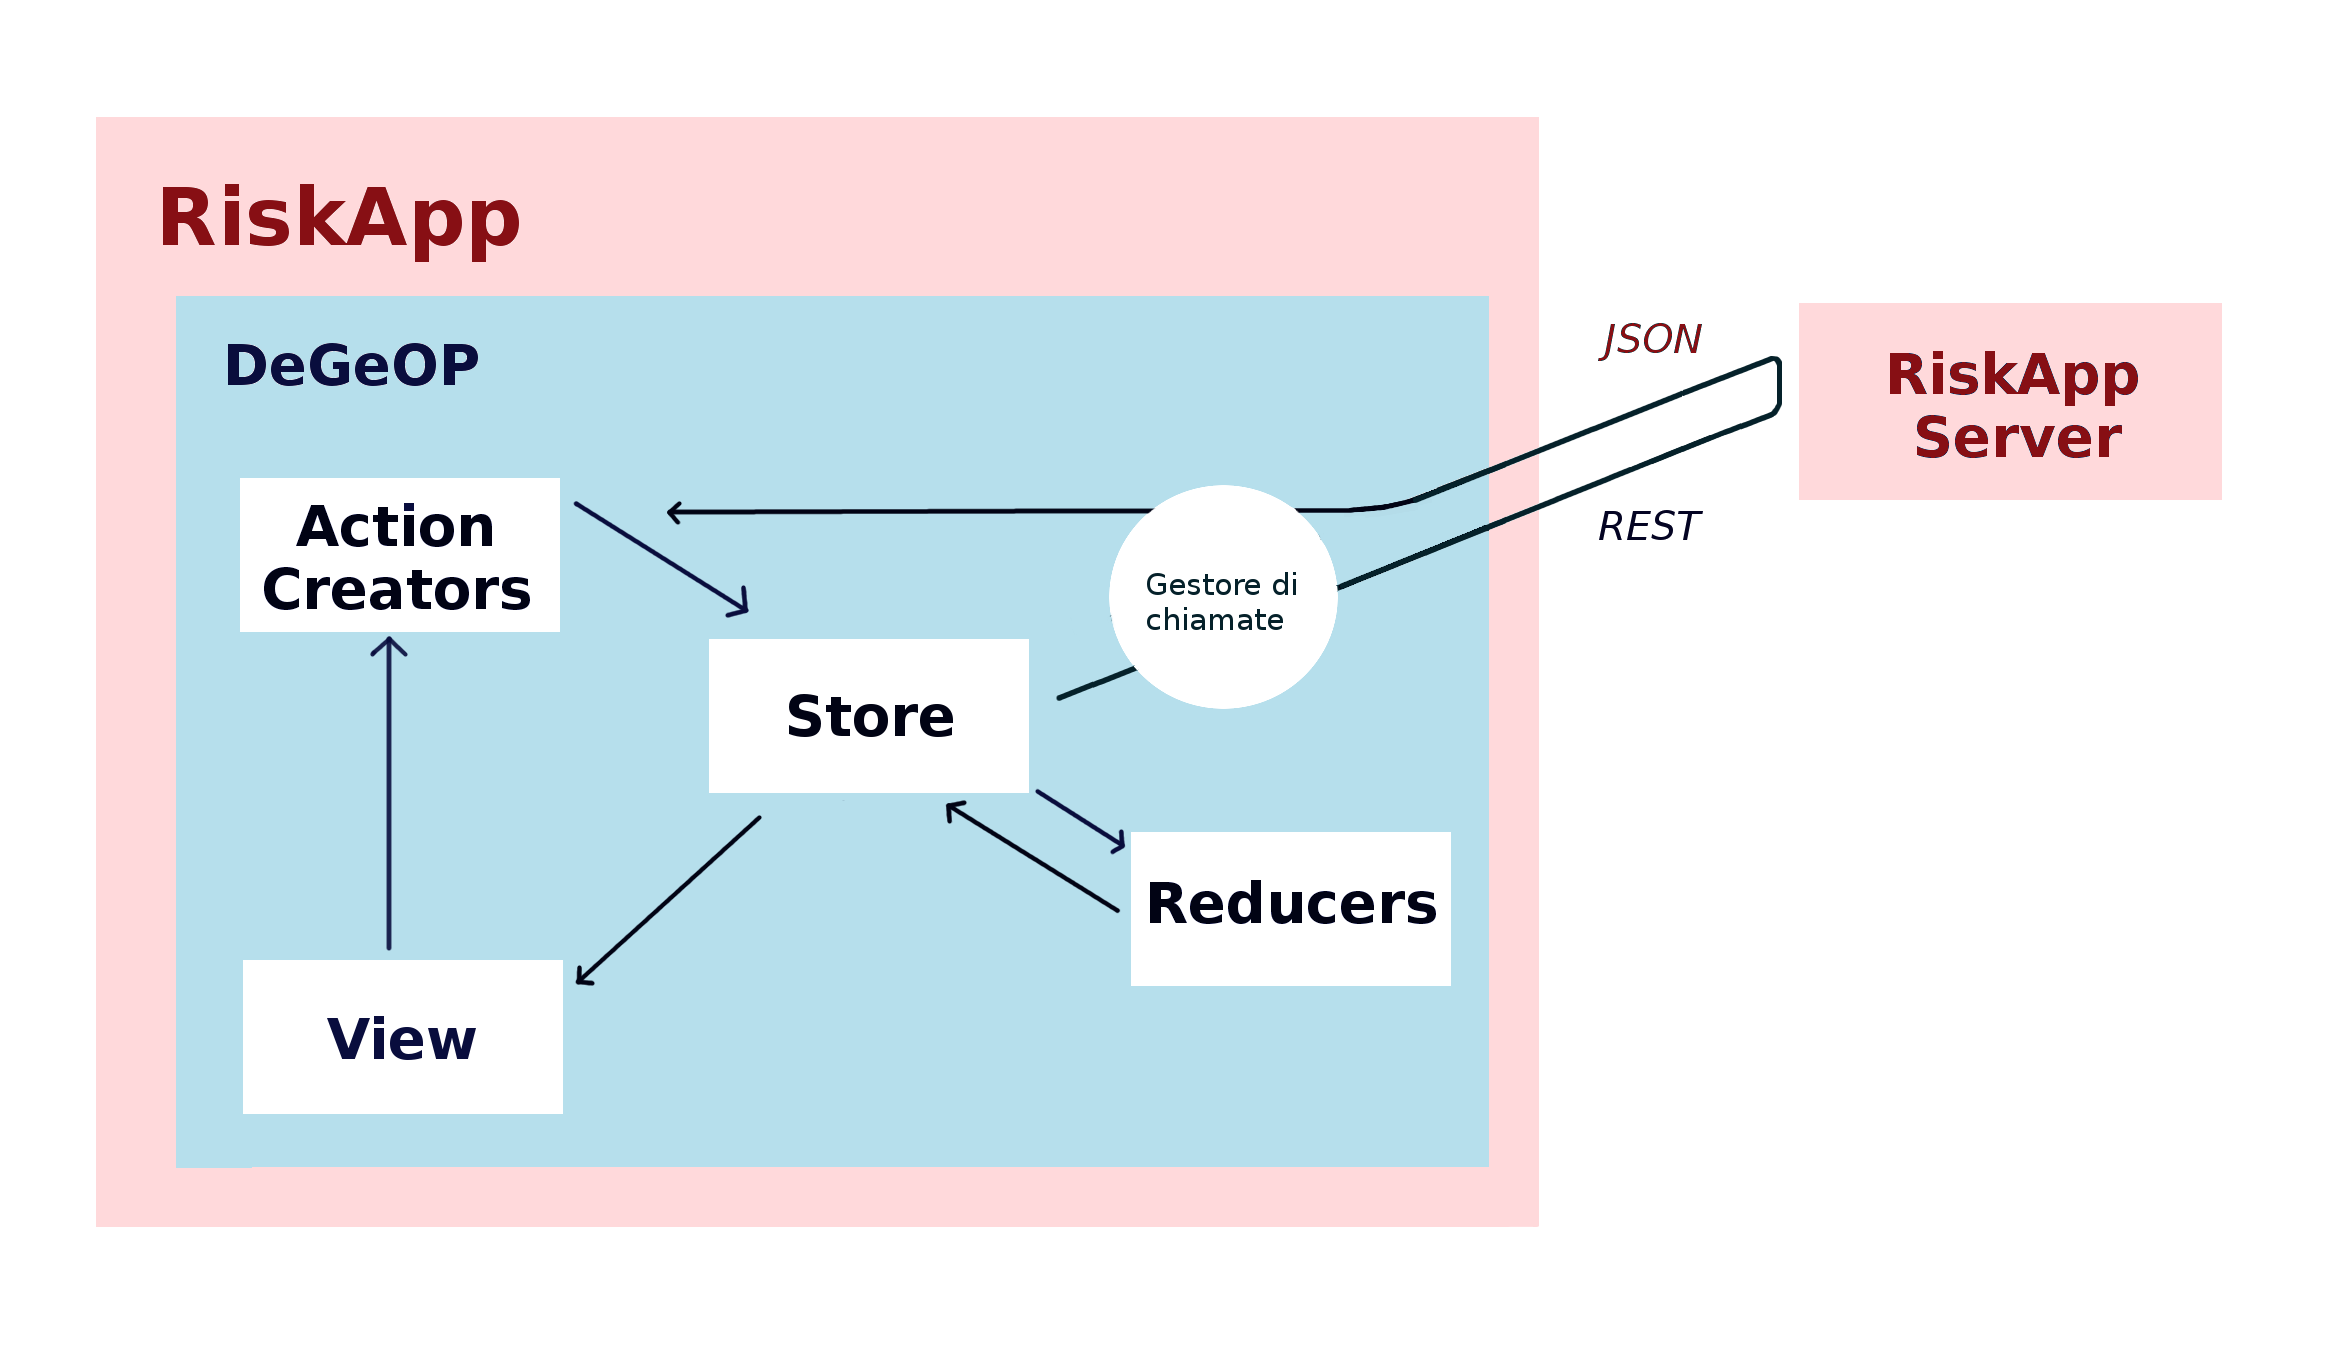
\includegraphics[width=\textwidth]{img/ArchitetturaBase.png}
	\caption{Architettura di base}
\end{figure}



	\section{Componenti}
\subsection{Introduzione}
 Partendo da quanto descritto nel documento di \textit{Specifica Tecnica}, è stato fatto uno studio approfondito delle tecnologie da utilizzare, in modo da poter scendere ad un livello di dettaglio tale da permettere di definire con chiarezza e precisione (seppure mantenendo la sintassi UML) la codifica dell'applicazione da parte dei programmatori.\\
 Questo si nota ed esempio all'interno del \textit{ViewPkg}: l'utilizzo di React, ha permesso:
 \begin{itemize}
	\item buon riutilizzo di codice, consentendo di ridurre fortemente il numero di componenti presentazionali che erano state progettate ad alto livello;
	\item semplificazione della procedura di costruzione dell'interfaccia grafica, grazie al principio di React "lifting state up", che consente la strutturazione dell'interfaccia in maniera fortemente modulare dal punto di vista puramente presentazionale, ma centralizzata dal punto di vista delle informazioni.
\end{itemize}
% v: 17
\subsection{DeGeOP}
\label{pkg::DeGeOP}
\begin{figure}[H]
	\centering
	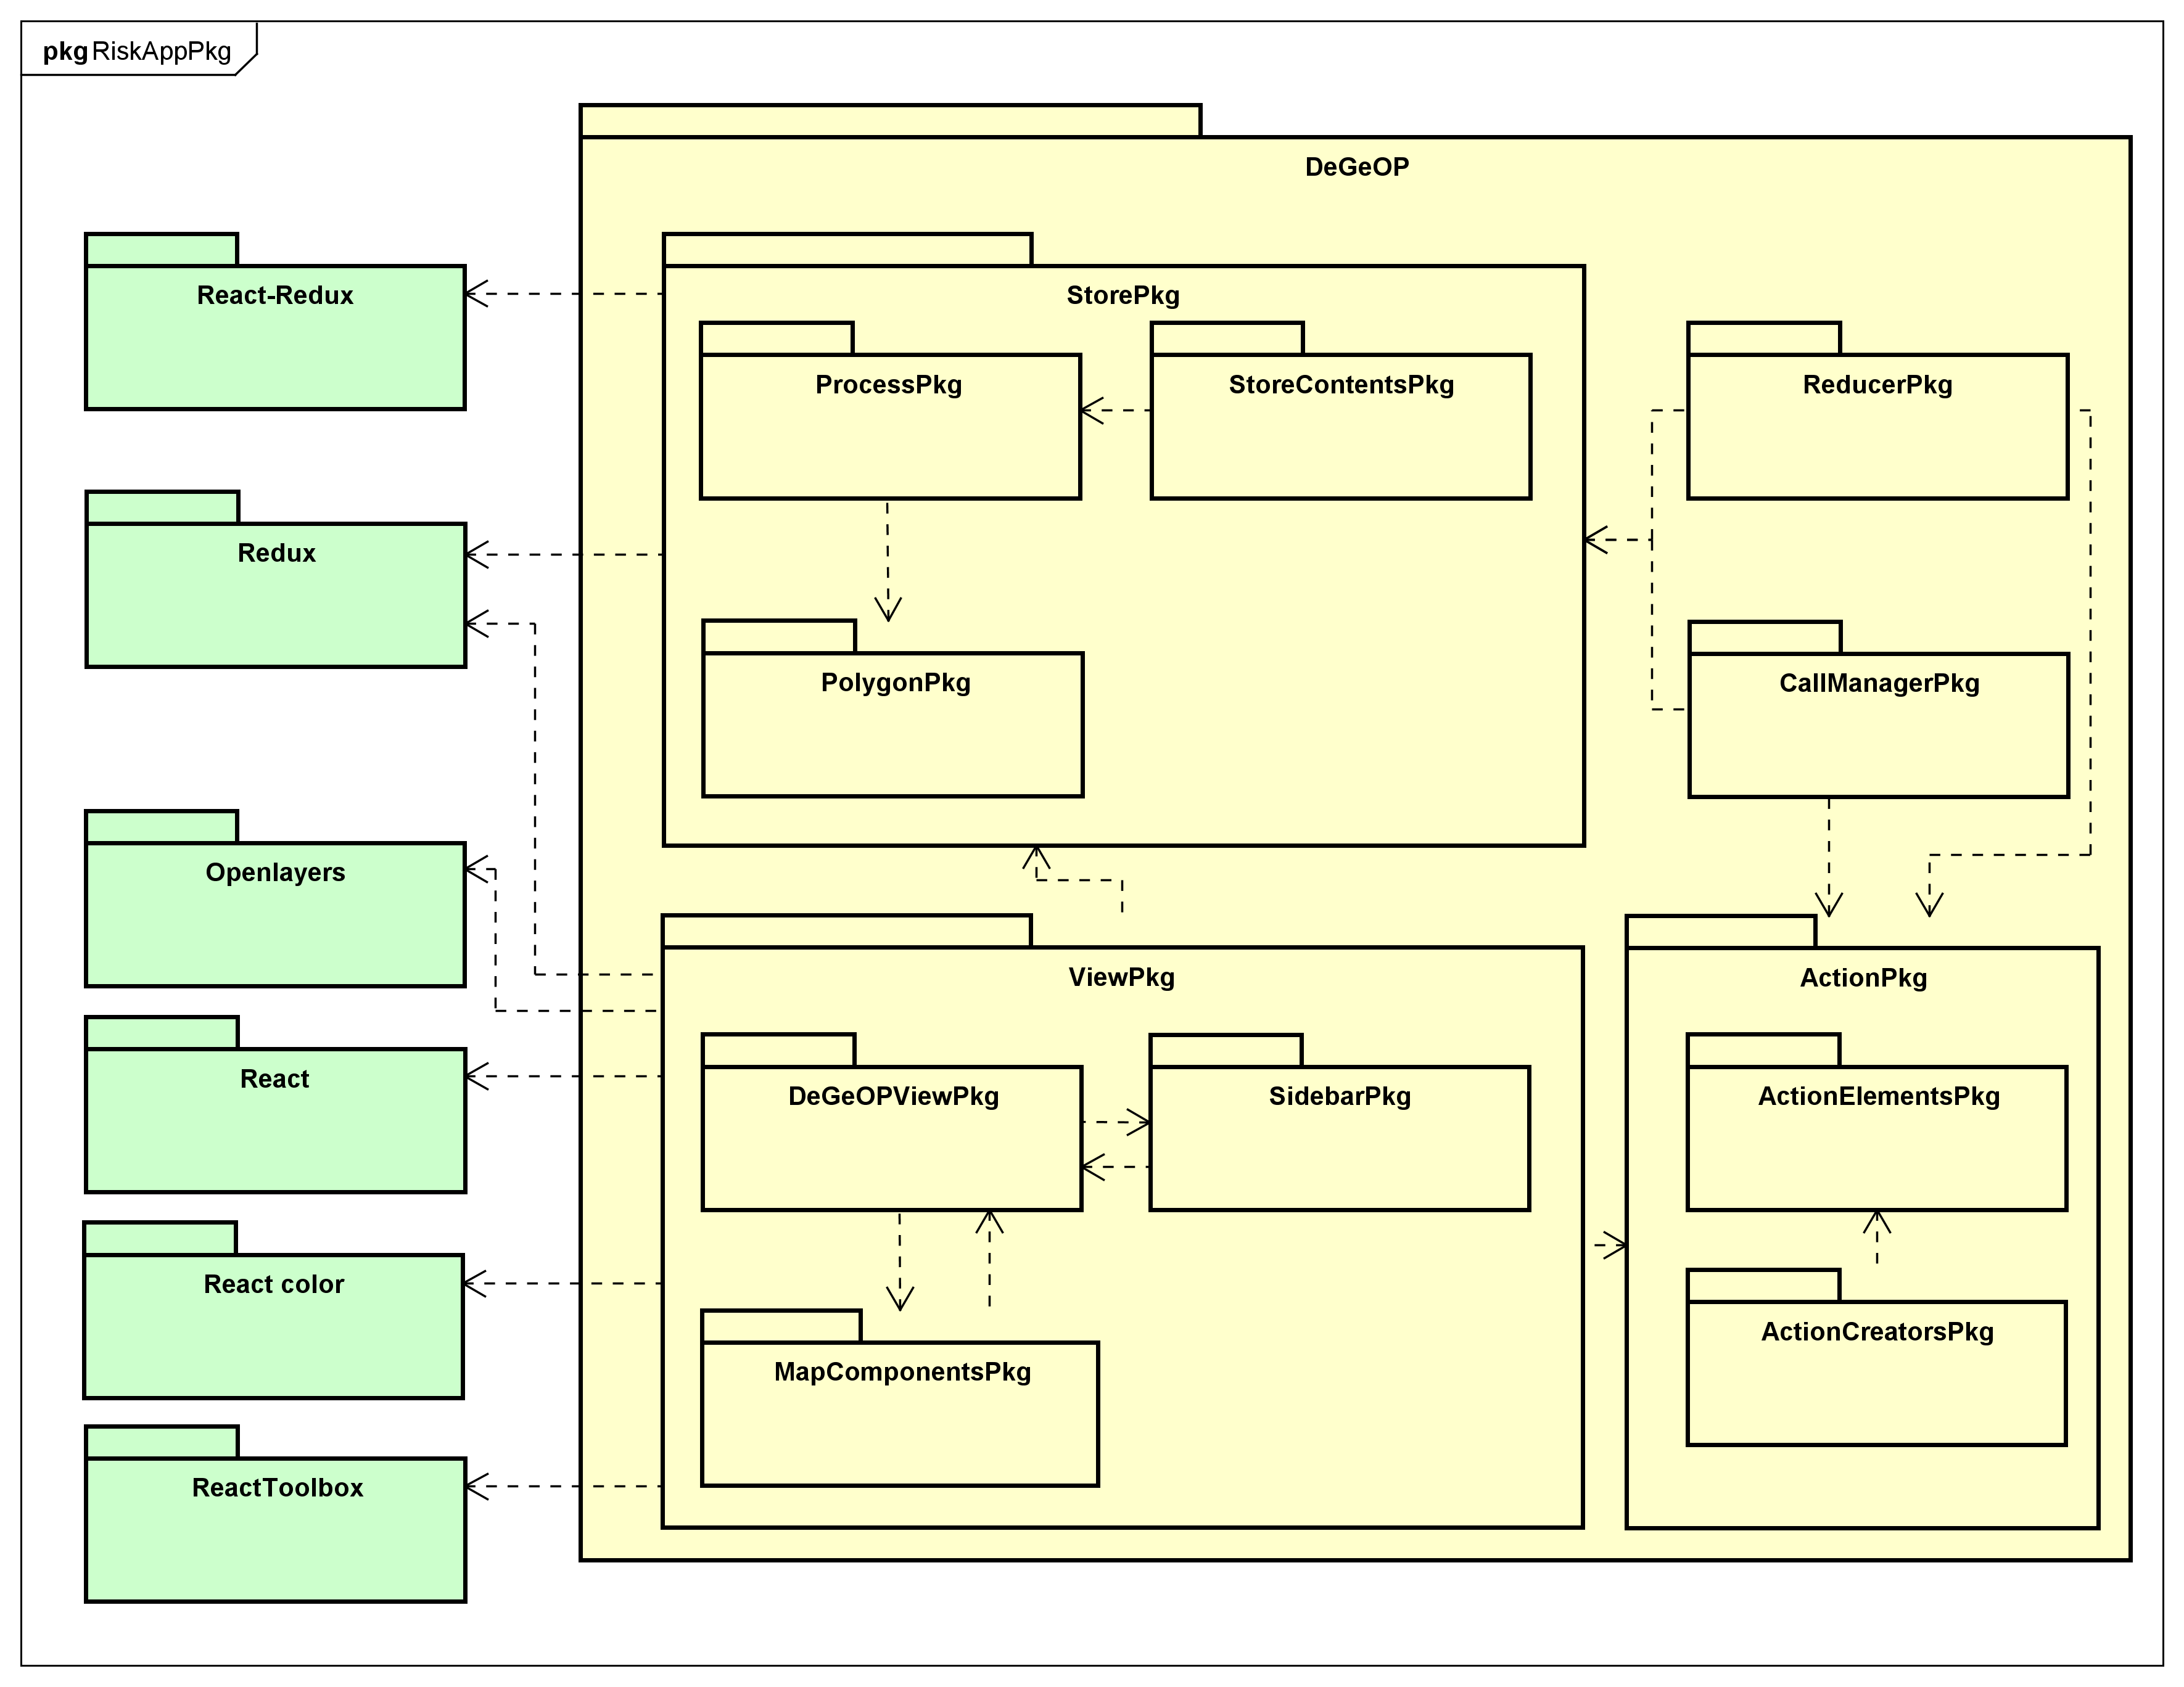
\includegraphics[width=\textwidth]{img/PkgDiagram/DeGeOPPkg.png}
	\caption{Schema componente DeGeOP}
\end{figure}
\subsubsection{Informazioni sul package}
\begin{itemize}
	\item \textbf{descrizione:} racchiude tutte le componenti necessarie per il front-end del prodotto;
	\item \textbf{package contenuti:}
	\begin{itemize}
		\item DeGeOP::\hyperref[pkg::ActionPkg]{ActionPkg};
		\item DeGeOP::\hyperref[pkg::CallManagerPkg]{CallManagerPkg};
		\item DeGeOP::\hyperref[pkg::ReducerPkg]{ReducerPkg};
		\item DeGeOP::\hyperref[pkg::StorePkg]{StorePkg};
		\item DeGeOP::\hyperref[pkg::ViewPkg]{ViewPkg}.
	\end{itemize}
\end{itemize}
\newpage
\subsection{DeGeOP::StorePkg}
\label{pkg::StorePkg}
\begin{figure}[H]
	\centering
	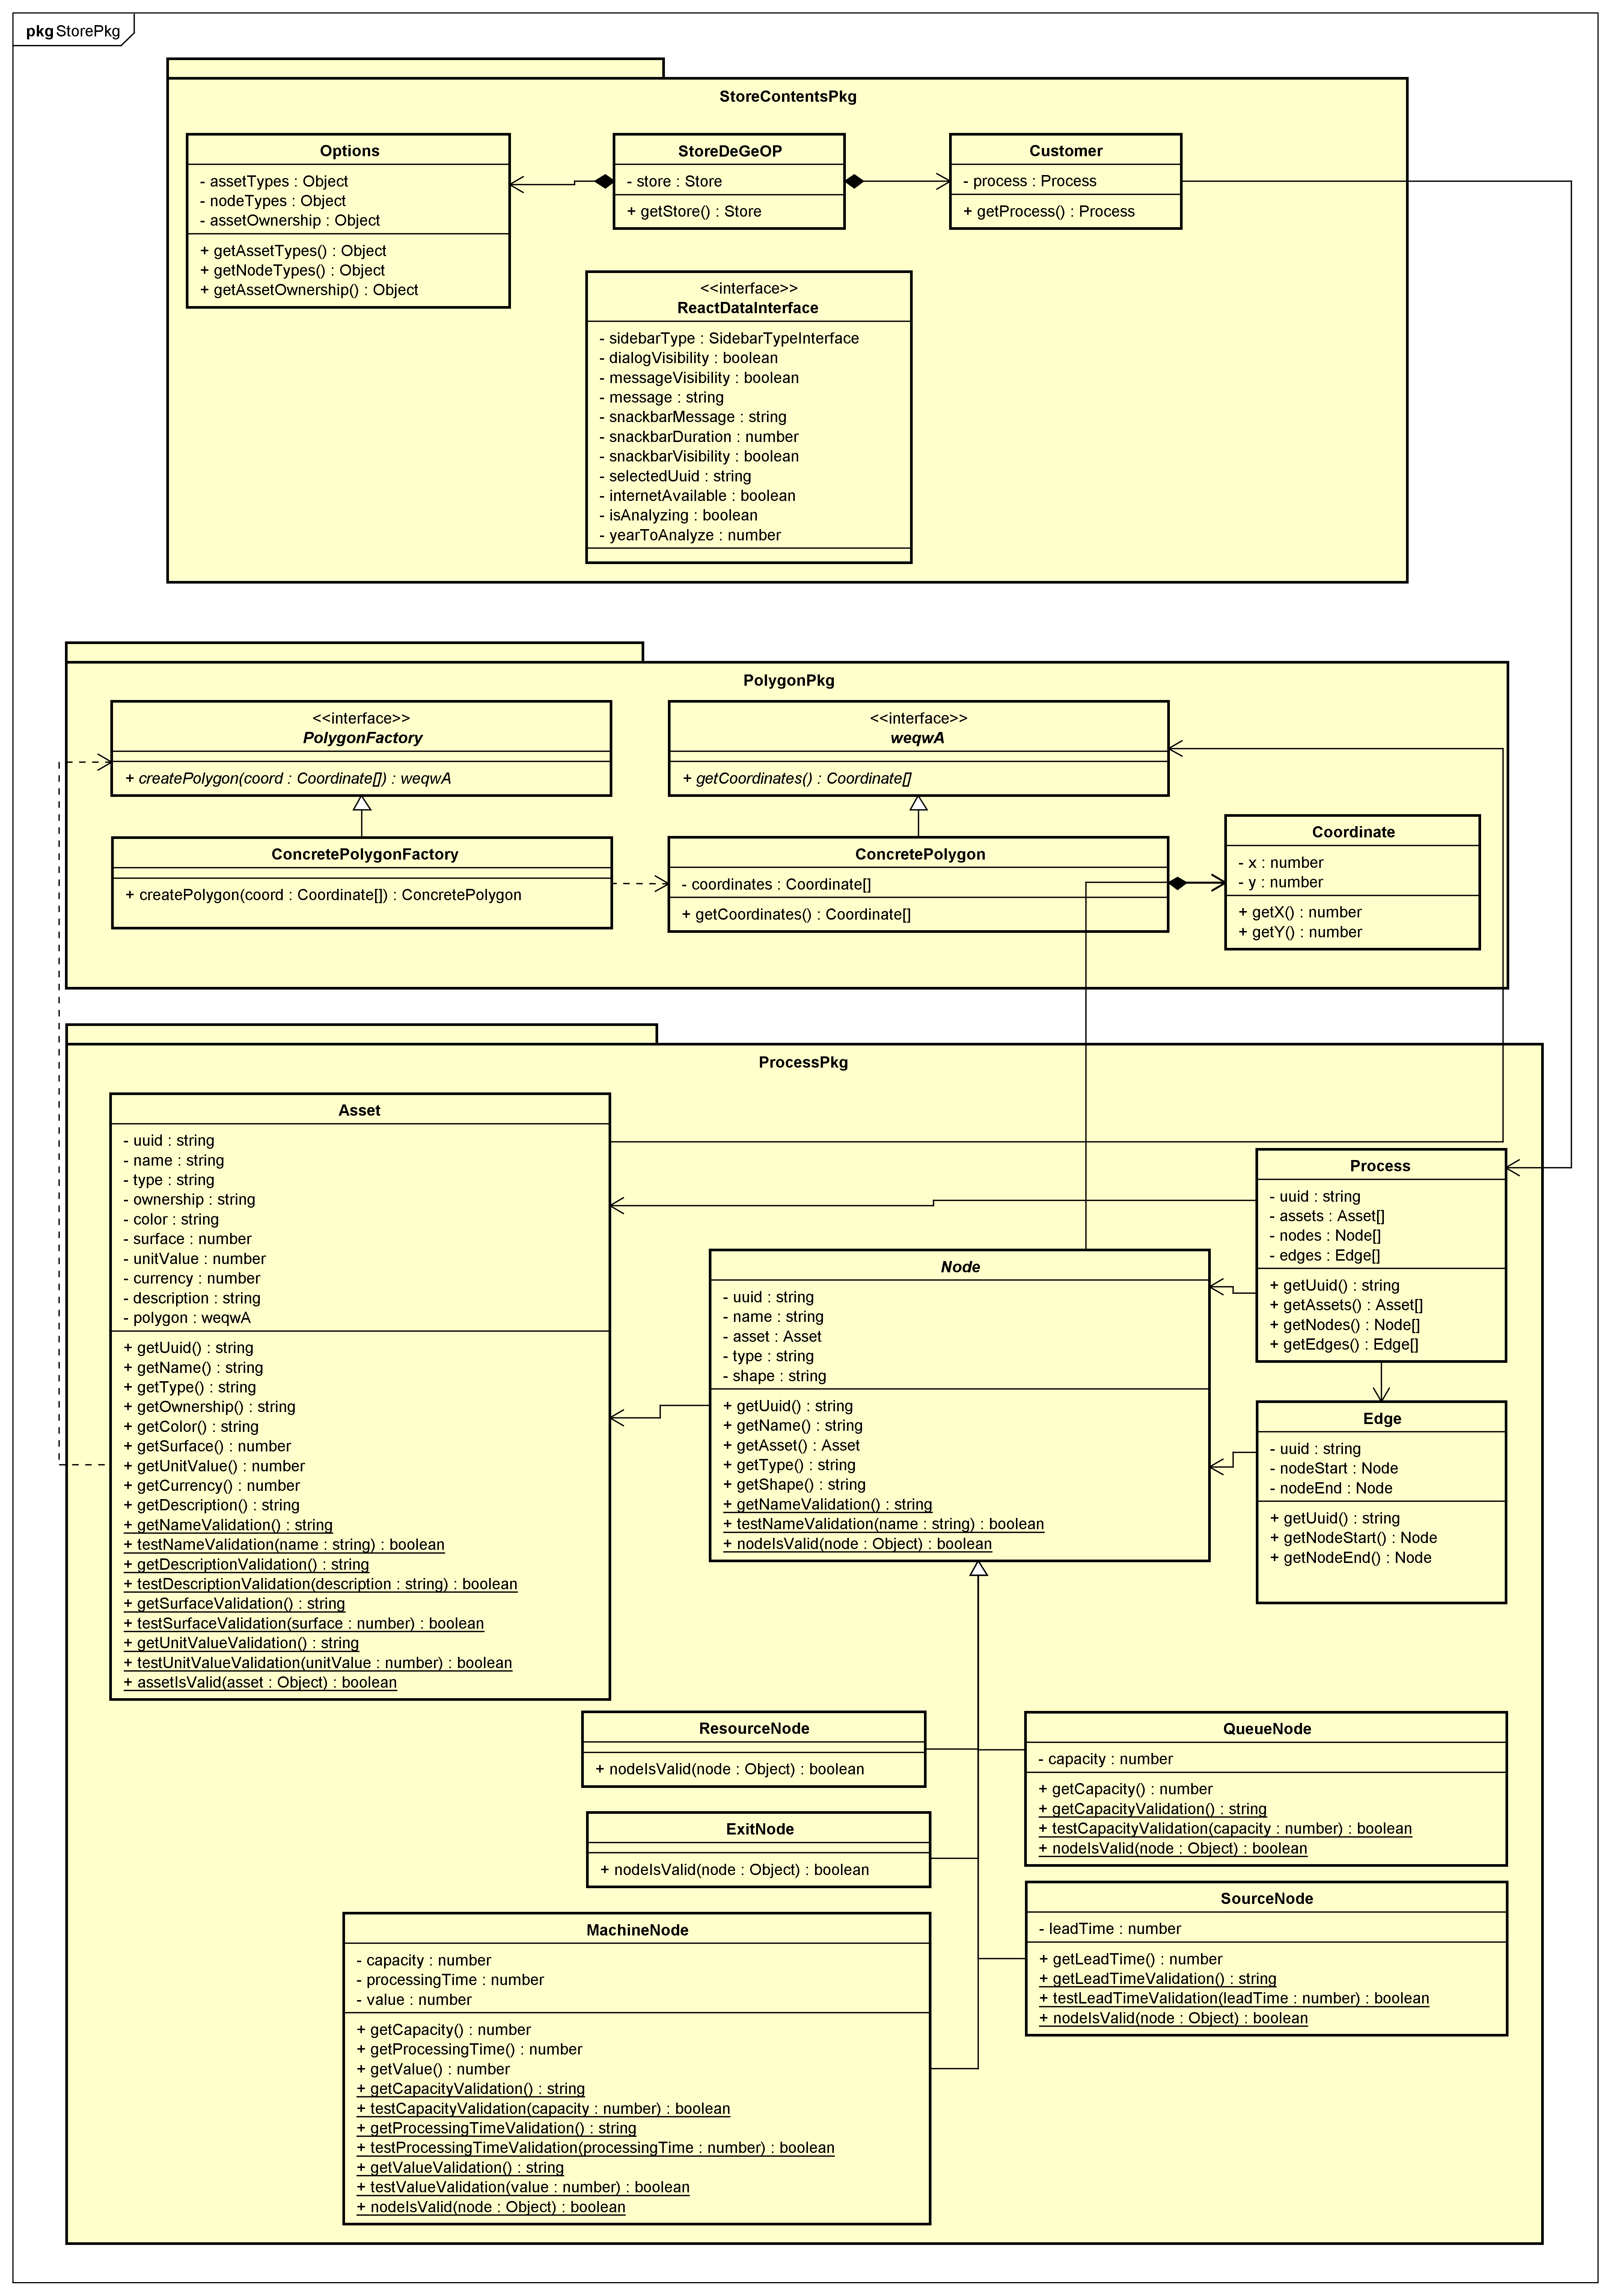
\includegraphics[width=\textwidth]{img/PkgDiagram/StorePkg.png}
	\caption{Schema componente DeGeOP::StorePkg}
\end{figure}
\subsubsection{Informazioni sul package}
\begin{itemize}
	\item \textbf{descrizione:} racchiude le componenti utilizzate per la memorizzazione e rappresentazione dei dati;
	\item \textbf{padre:} \hyperref[pkg::DeGeOP]{DeGeOP};
	\item \textbf{package contenuti:}
	\begin{itemize}
		\item StorePkg::\hyperref[pkg::PolygonPkg]{PolygonPkg};
		\item StorePkg::\hyperref[pkg::ProcessPkg]{ProcessPkg};
		\item StorePkg::\hyperref[pkg::StoreContentsPkg]{StoreContentsPkg}.
	\end{itemize}
	\item \textbf{interazioni con altri package:} 
	\begin{itemize}
		\item IN CallManagerPkg: subscribe sullo store;
		\item IN ReducerPkg: applicazione di cambiamenti di stato;
		\item IN ViewPkg: subscribe sullo store;
		\item OUT React-Redux: utilizzo di Provider per evitare di passare lo store come proprietà alle componenti React;
		\item OUT Redux: creazione Store utilizzando il metodo createStore().
	\end{itemize}
\end{itemize}
\newpage
\subsection{DeGeOP::StorePkg::StoreContentsPkg}
\label{pkg::StoreContentsPkg}
\subsubsection{Informazioni sul package}
\begin{itemize}
	\item \textbf{descrizione:} racchiude le componenti che implementano il concetto di store dell'architettura Redux;
	\item \textbf{padre:} \hyperref[pkg::StorePkg]{StorePkg};
	\item \textbf{interazioni con altri package:} 
	\begin{itemize}
		\item OUT AnalysisPkg: riferimento ad analisi di danno;
		\item OUT ProcessPkg: riferimento a processo;
		\item OUT React-Redux: utilizzo del Provider;
		\item OUT Redux: creazione store.
	\end{itemize}
	\item \textbf{classi contenute:}
	\begin{itemize}
		\item Customer;
		\item Options;
		\item ReactDataInterface;
		\item StoreDeGeOP.
	\end{itemize}
\end{itemize}
\subsubsection{Classi}
\paragraph{Customer}
\begin{itemize}
	\begin{figure}[H]
		\centering
		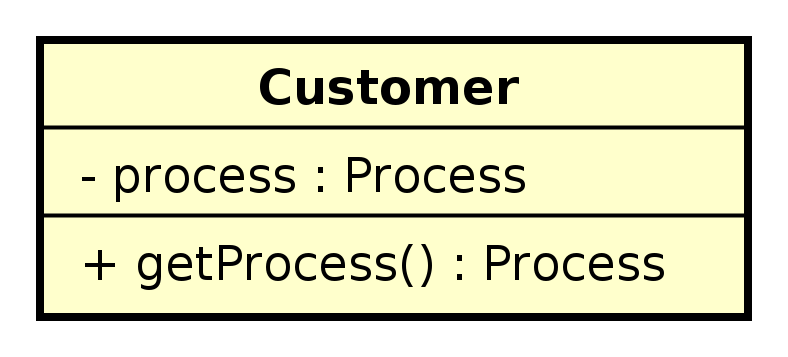
\includegraphics[width=0.3\textwidth]{./img/Customer.png}
		\caption{Diagramma classe Customer}
	\end{figure}
	\item \textbf{descrizione:} rappresenta l'assicurando;
	\item \textbf{utilizzo:} viene utilizzato nello Store per memorizzare l'assicurando;
	\item \textbf{attributi:}
	\begin{itemize}
		\item -process : Process\begin{itemize}
			\item rappresenta il processo produttivo dell'assicurando.\end{itemize}
	\end{itemize}
	\item \textbf{metodi:}
	\begin{itemize}
		\item +getProcess() : Process\newline
		il metodo restituisce il processo produttivo dell'assicurando
	\end{itemize}
\end{itemize}
\paragraph{Options}
\begin{itemize}
	\begin{figure}[H]
		\centering
		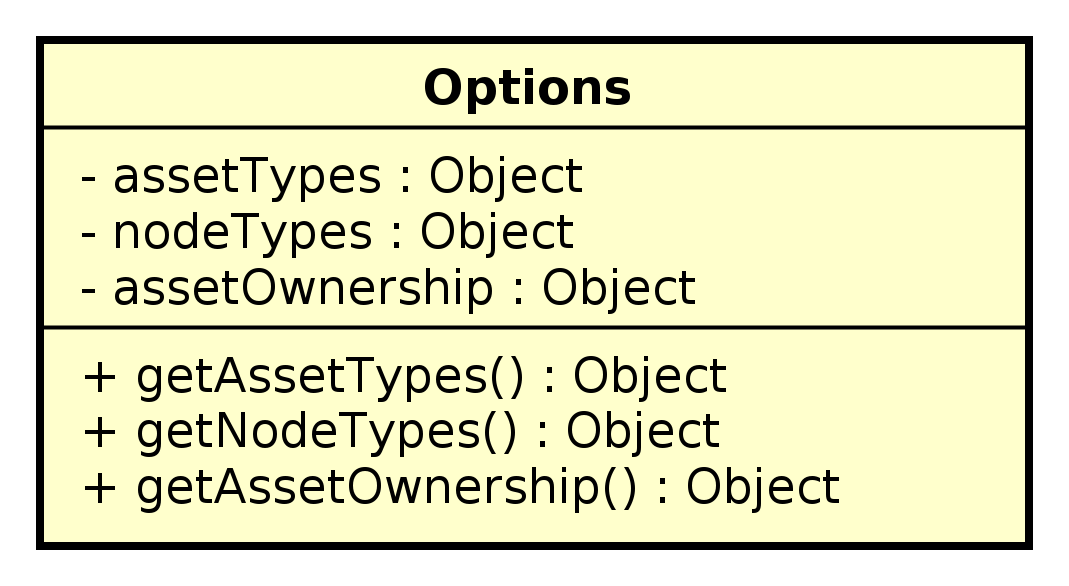
\includegraphics[width=0.3\textwidth]{./img/Options.png}
		\caption{Diagramma classe Options}
	\end{figure}
	\item \textbf{descrizione:} classe contenente le associazioni tra codice e valore dei campi dati degli altri elementi dello store;
	\item \textbf{utilizzo:} viene utilizzata per associare codice e valore dei campi dati degli altri elementi dello store;
	\item \textbf{attributi:}
	\begin{itemize}
		\item -assetOwnership : Object\begin{itemize}
			\item associazione chiave valore delle tipologie di soggetti di appartenenza dell'asset.\end{itemize}
		\item -assetTypes : Object\begin{itemize}
			\item associazione chiave valore delle tipologie di materiale dell'asset.\end{itemize}
		\item -nodeTypes : Object\begin{itemize}
			\item associazione chiave valore delle tipologie di materiale del nodo.\end{itemize}
	\end{itemize}
	\item \textbf{metodi:}
	\begin{itemize}
		\item +getAssetOwnership() : Object\newline
		il metodo ritorna l'oggetto assetOwnership
		\item +getAssetTypes() : Object\newline
		il metodo ritorna l'oggetto assetTypes
		\item +getNodeTypes() : Object\newline
		il metodo ritorna l'oggetto nodeTypes
	\end{itemize}
	\item \textbf{relazioni con altre classi:} 
	\begin{itemize}
		\item IN OptionReducer;
		\item IN StoreDeGeOP.
	\end{itemize}
\end{itemize}
\paragraph{ReactDataInterface}
\begin{itemize}
	\item \textbf{descrizione:} rappresenta l'interfaccia per reactData;
	\item \textbf{utilizzo:} l'interfaccia contiene dati riguardanti il comportamento della view;
	\item \textbf{attributi:}
	\begin{itemize}
		\item -dialogVisibility : boolean\begin{itemize}
			\item indica se la dialog viene visualizzata o meno.\end{itemize}
		\item -internetAvailable : boolean\begin{itemize}
			\item indica la presenza della connessione ad internet.\end{itemize}
		\item -isAnalyzing : boolean\begin{itemize}
			\item indica se un'analisi è in corso.\end{itemize}
		\item -message : string\begin{itemize}
			\item contiene il messaggio che viene visualizzato.\end{itemize}
		\item -messageVisibility : boolean\begin{itemize}
			\item indica se viene visualizzato o meno un messaggio.\end{itemize}
		\item -selectedUuid : string\begin{itemize}
			\item rappresenta l'uuid dell'oggetto selezionato.\end{itemize}
		\item -sidebarType : SidebarTypeInterface\begin{itemize}
			\item indica la tipologia di sidebar.\end{itemize}
		\item -snackbarDuration : number\begin{itemize}
			\item indica il tempo di visualizzazione della snackbar.\end{itemize}
		\item -snackbarMessage : string\begin{itemize}
			\item indica il messaggio da visualizzare nella snackbar.\end{itemize}
		\item -snackbarVisibility : boolean\begin{itemize}
			\item indica se la snackbar viene visualizzata o meno.\end{itemize}
		\item -yearToAnalyze : number\begin{itemize}
			\item rappresenta l'anno da analizzare.\end{itemize}
	\end{itemize}
\end{itemize}
\paragraph{StoreDeGeOP}
\begin{itemize}
	\begin{figure}[H]
		\centering
		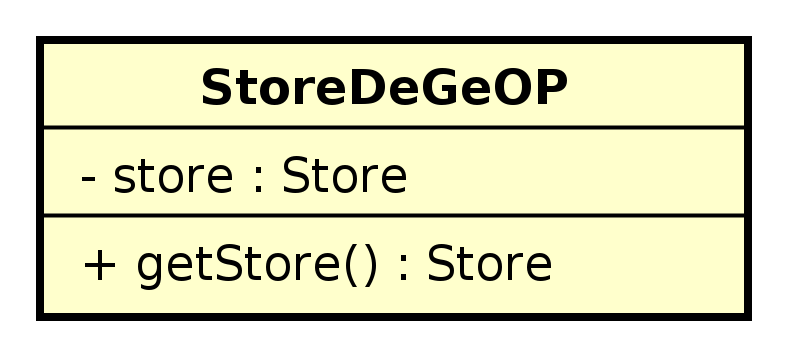
\includegraphics[width=0.3\textwidth]{./img/StoreDeGeOP.png}
		\caption{Diagramma classe StoreDeGeOP}
	\end{figure}
	\item \textbf{descrizione:} rappresenta una classe che incapsula uno Store creato utilizzando Redux;
	\item \textbf{utilizzo:} viene utilizzato per memorizzare lo stato dell'applicazione.
	Le componenti che effettuano il subscribe sullo Store verranno notificate ad ogni cambiamento di stato dello Store;
	\item \textbf{attributi:}
	\begin{itemize}
		\item -customer : Customer\begin{itemize}
			\item rappresenta il cliente che gestiamo.\end{itemize}
		\item -store : Object\begin{itemize}
			\item rappresenta l'oggetto Store creato utilizzando Redux.\end{itemize}
	\end{itemize}
	\item \textbf{metodi:}
	\begin{itemize}
		\item +getStore() : Object\newline
		il metodo restituisce lo store creato utilizzando Redux
	\end{itemize}
	\item \textbf{relazioni con altre classi:} 
	\begin{itemize}
		\item IN Reducer;
		\item OUT Options.
	\end{itemize}
\end{itemize}
\newpage
\subsection{DeGeOP::StorePkg::ProcessPkg}
\label{pkg::ProcessPkg}
\subsubsection{Informazioni sul package}
\begin{itemize}
	\item \textbf{descrizione:} racchiude le componenti necessarie alla rappresentazione del processo produttivo dell'assicurando;
	\item \textbf{padre:} \hyperref[pkg::StorePkg]{StorePkg};
	\item \textbf{interazioni con altri package:} 
	\begin{itemize}
		\item IN StoreContentsPkg: riferimento a processo;
		\item OUT PolygonPkg: riferimento ad un poligono.
	\end{itemize}
	\item \textbf{classi contenute:}
	\begin{itemize}
		\item Asset;
		\item Edge;
		\item ExitNode;
		\item MachineNode;
		\item Node;
		\item Process;
		\item QueueNode;
		\item ResourceNode;
		\item SourceNode.
	\end{itemize}
\end{itemize}
\subsubsection{Classi}
\paragraph{Asset}
\begin{itemize}
	\begin{figure}[H]
		\centering
		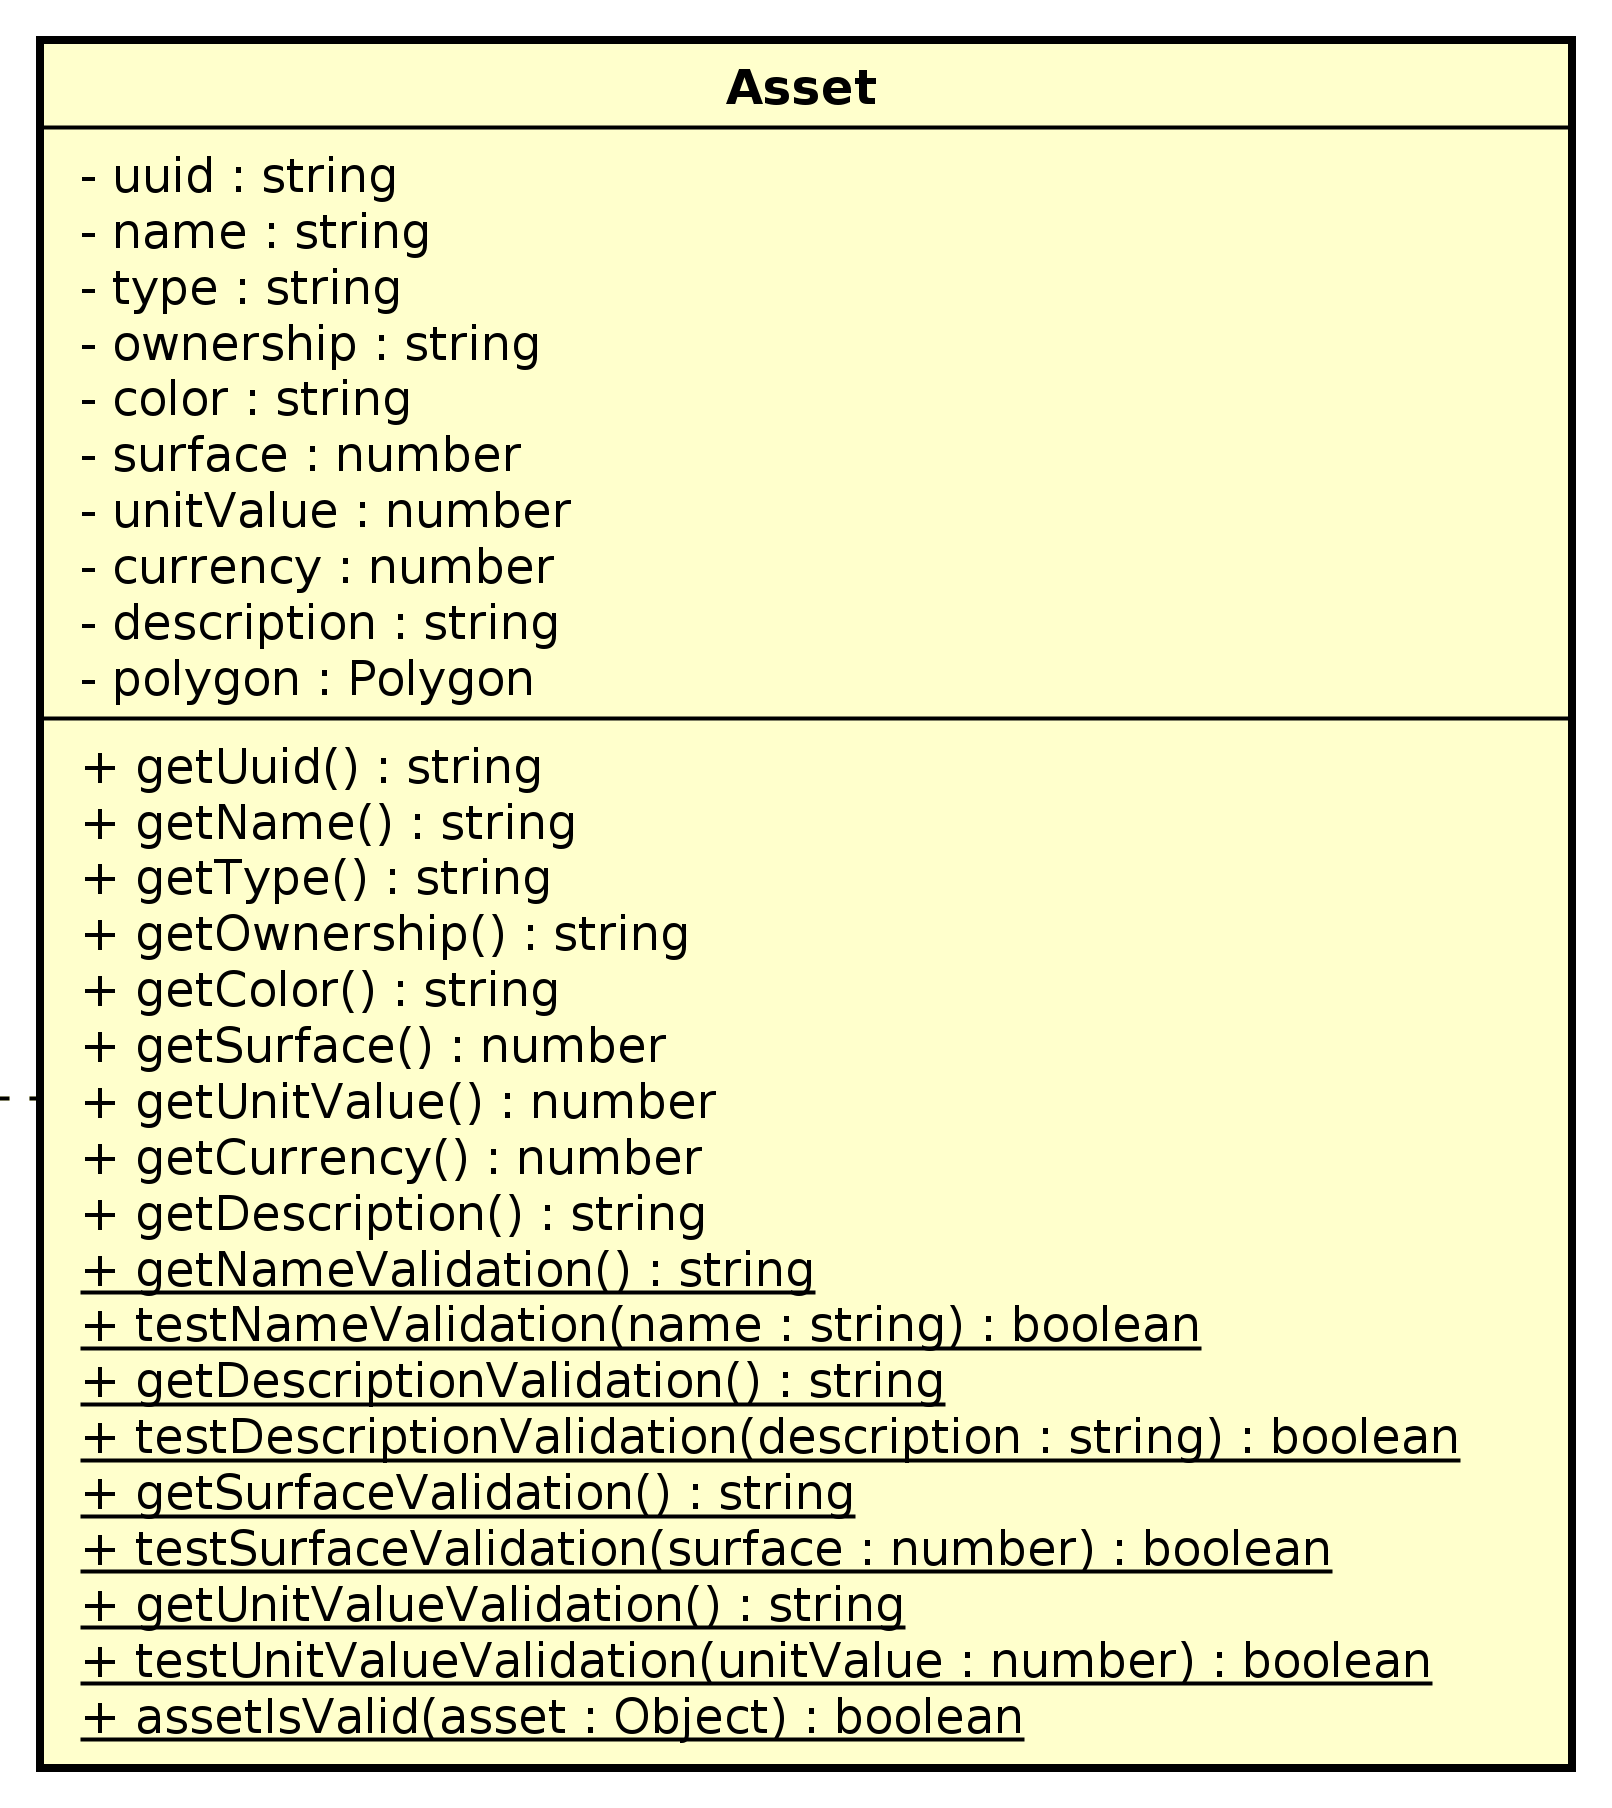
\includegraphics[width=0.3\textwidth]{./img/Asset.png}
		\caption{Diagramma classe Asset}
	\end{figure}
	\item \textbf{descrizione:} rappresenta un fabbricato di interesse per il processo produttivo dell'assicurando;
	\item \textbf{utilizzo:} sono contenuti all'interno di Process;
	\item \textbf{attributi:}
	\begin{itemize}
		\item -color : string\begin{itemize}
			\item indica il colore dell'asset.\end{itemize}
		\item -currency : number\begin{itemize}
			\item indica la valuta utilizzata.\end{itemize}
		\item -description : string\begin{itemize}
			\item rappresenta la descrizione dell'asset.\end{itemize}
		\item -name : string\begin{itemize}
			\item rappresenta il nome dell'asset.\end{itemize}
		\item -ownership : string\begin{itemize}
			\item rappresenta l'appartenenza dell'asset.\end{itemize}
		\item -surface : number\begin{itemize}
			\item rappresenta la dimensione, in mq, dell'asset.\end{itemize}
		\item -type : string\begin{itemize}
			\item rappresenta la tipologia dell'asset.\end{itemize}
		\item -unitValue : string\begin{itemize}
			\item indica il valore economico dell'asset.\end{itemize}
		\item -uuid : string\begin{itemize}
			\item rappresenta l'identificativo dell'asset (uuid).\end{itemize}
	\end{itemize}
	\item \textbf{metodi:}
	\begin{itemize}
		\item +assetIsValid(asset) : boolean\newline
		il metodo testa che i parametri con cui l'asset sta per essere creato siano validi
		\begin{itemize}
			\item asset : Object\\
			oggetto contenente i parametri di un Asset che dovrà essere validato.
		\end{itemize}
		\item +getColor() : string\newline
		il metodo ritorna il colore dell'asset
		\item +getCurrency() : number\newline
		il metodo ritorna la valuta utilizzata per l'asset
		\item +getDescription() : string\newline
		il metodo ritorna la descrizione dell'asset
		\item +getDescriptionValidation() : string\newline
		il metodo ritorna l'espressione regolare che indica una stringa non contenente le seguenti caratteristiche: vuota; più lunga di 5000 caratteri; inizia e/o finisce con uno spazio; contiene caratteri speciali
		diversi dall’apostrofo
		\item +getName() : string\newline
		ritorna il nome dell'asset
		\item +getNameValidation() : string\newline
		il metodo ritorna l'espressione regolare che indica una stringa non contenente le seguenti caratteristiche: più lunga di 50 caratteri; inizia e/o finisce con uno spazio; contiene caratteri speciali.
		\item +getOwnership() : string\newline
		il metodo ritorna l'appartenenza dell'asset
		\item +getSurface() : number\newline
		il metodo ritorna la dimensione dell'asset
		\item +getSurfaceValidation() : string\newline
		il metodo ritorna l'espressione regolare che indica una stringa non contenente le seguenti caratteristiche:vuota; più lunga di 5 cifre per la parte intera; più di 2 per la parte decimale;
		
		\item +getType() : string\newline
		il metodo ritorna la tipologia dell'asset
		\item +getUnitValue() : string\newline
		il metodo ritorna il valore economico dell'asset
		\item +getUnitValueValidation() : string\newline
		il metodo ritorna l'espressione regolare che indica una stringa non contenente le seguenti caratteristiche: vuota; più lunga di 5 cifre per la parte intera; più di 2 per la parte decimale
		\item +getUuid() : string\newline
		il metodo ritorna l'uuid dell'asset
		\item +testDescriptionValidation(description) : boolean\newline
		il metodo ritorna true solamente se il valore ricevuto in input, come parametro, è ritenuto valido.
		\begin{itemize}
			\item description : string\\
			rappresenta la descrizione dell'asset.
		\end{itemize}
		\item +testNameValidation(name) : boolean\newline
		il metodo ritorna true solamente se il valore ricevuto in input, come parametro, è ritenuto valido.
		\begin{itemize}
			\item name : string\\
			rappresenta il nome dell'asset.
		\end{itemize}
		\item +testSurfaceValidation(surface) : boolean\newline
		il metodo ritorna true solamente se il valore ricevuto in input, come parametro, è ritenuto valido.
		\begin{itemize}
			\item surface : number\\
			rappresenta la dimensione, in mq, dell'asset.
		\end{itemize}
		\item +testUnitValueValidation(unitValue) : boolean\newline
		il metodo ritorna true solamente se il valore ricevuto in input, come parametro, è ritenuto valido.
		\begin{itemize}
			\item unitValue : number\\
			indica il valore economico dell'asset.
		\end{itemize}
	\end{itemize}
	\item \textbf{relazioni con altre classi:} 
	\begin{itemize}
		\item IN AssetReducer.
	\end{itemize}
\end{itemize}
\paragraph{Edge}
\begin{itemize}
	\begin{figure}[H]
		\centering
		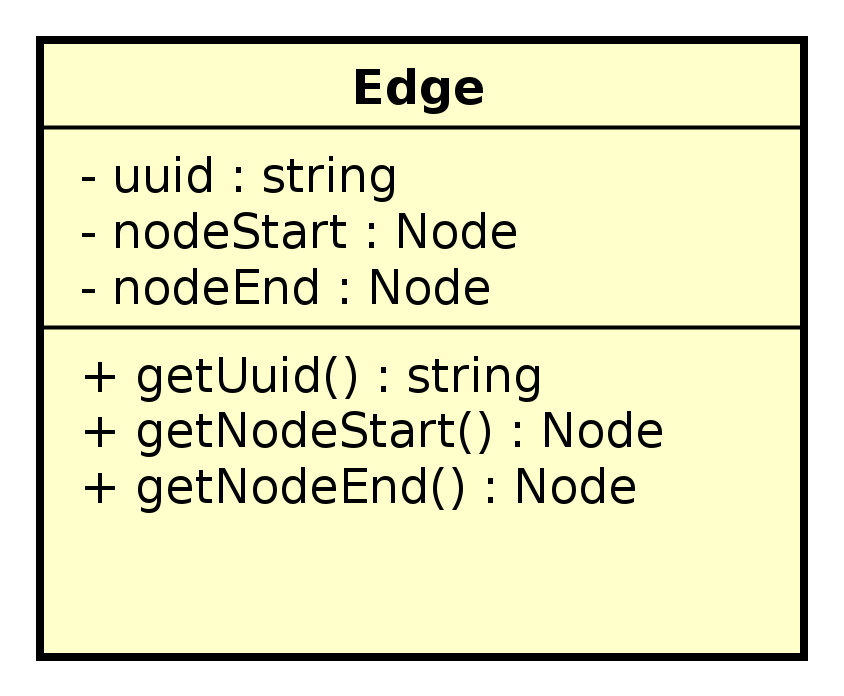
\includegraphics[width=0.3\textwidth]{./img/Edge.png}
		\caption{Diagramma classe Edge}
	\end{figure}
	\item \textbf{descrizione:} rappresenta un arco che collega due nodi tra di loro; un arco indica che i nodi sono in correlazione tra di loro;
	\item \textbf{utilizzo:} è contenuto all'interno di Process;
	\item \textbf{attributi:}
	\begin{itemize}
		\item -nodeEnd : Node\begin{itemize}
			\item rappresenta il nodo di arrivo.\end{itemize}
		\item -nodeStart : Node\begin{itemize}
			\item rappresenta il nodo di partenza.\end{itemize}
		\item -uuid : string\begin{itemize}
			\item rappresenta il codice identificativo dell'arco (uuid).\end{itemize}
	\end{itemize}
	\item \textbf{metodi:}
	\begin{itemize}
		\item +getNodeEnd() : Node\newline
		il metodo restituisce il nodo di arrivo
		\item +getNodeStart() : Node\newline
		il metodo restituisce il nodo di partenza
		\item +getUuid() : string\newline
		il metodo restituisce il codice identificativo dell'arco (uuid)
	\end{itemize}
	\item \textbf{relazioni con altre classi:} 
	\begin{itemize}
		\item IN EdgeReducer.
	\end{itemize}
\end{itemize}
\paragraph{ExitNode}
\begin{itemize}
	\begin{figure}[H]
		\centering
		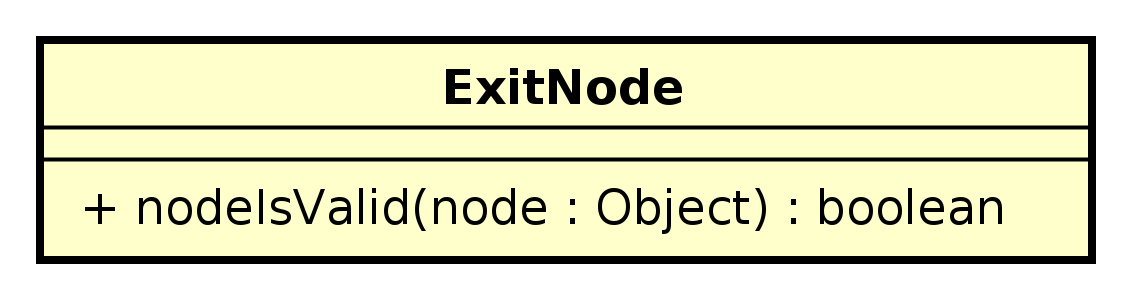
\includegraphics[width=0.3\textwidth]{./img/ExitNode.png}
		\caption{Diagramma classe ExitNode}
	\end{figure}
	\item \textbf{descrizione:} rappresenta un nodo di tipo Uscita;
	\item \textbf{utilizzo:} è contenuto all'interno di Process;
	\item \textbf{metodi:}
	\begin{itemize}
		\item +nodeIsValid() : boolean\newline
		il metodo testa che i parametri con cui il nodo sta per essere creato siano validi
	\end{itemize}
\end{itemize}
\paragraph{MachineNode}
\begin{itemize}
	\begin{figure}[H]
		\centering
		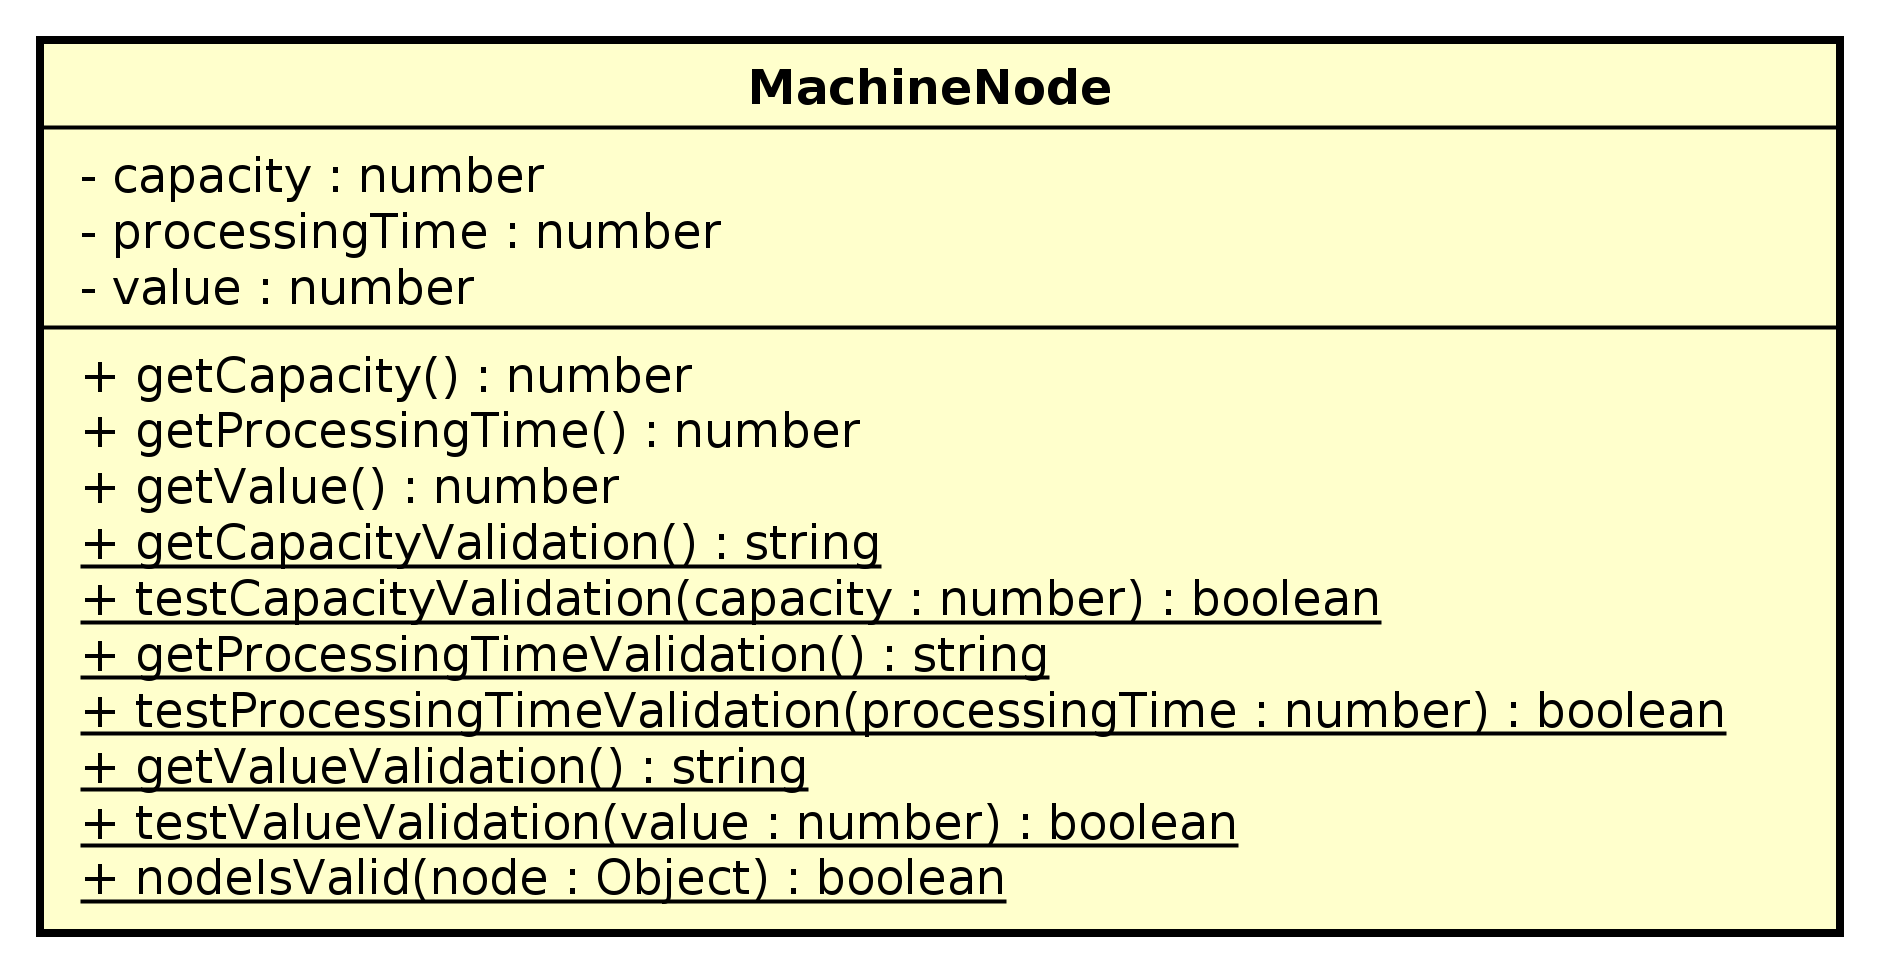
\includegraphics[width=0.3\textwidth]{./img/MachineNode.png}
		\caption{Diagramma classe MachineNode}
	\end{figure}
	\item \textbf{descrizione:} rappresenta un nodo di tipo Macchina;
	\item \textbf{utilizzo:} è contenuto all'interno di Process;
	\item \textbf{attributi:}
	\begin{itemize}
		\item -capacity : number\begin{itemize}
			\item rappresenta la capacità del nodo.\end{itemize}
		\item -processingTime : number\begin{itemize}
			\item rappresenta il tempo di processo del nodo.\end{itemize}
		\item -value : number\begin{itemize}
			\item rappresenta il valore del nodo.\end{itemize}
	\end{itemize}
	\item \textbf{metodi:}
	\begin{itemize}
		\item +getCapacity() : number\newline
		il metodo ritorna la capacità del nodo
		\item +getCapacityValidation() : string\newline
		il metodo ritorna l'espressione regolare che indica una stringa non contenente le seguenti caratteristiche: vuota; più lunga di 5 cifre per la parte intera; più di 2 per la parte decimale;
		\item +getProcessingTime() : number\newline
		il metodo ritorna il tempo di processo del nodo
		\item +getProcessingTimeValidation() : string\newline
		il metodo ritorna l'espressione regolare che indica una stringa non contenente le seguenti caratteristiche: vuota; più lunga di 5 cifre per la parte intera; più di 2 per la parte decimale;
		\item +getValue() : number\newline
		il metodo ritorna il valore del nodo
		\item +getValueValidation() : string\newline
		il metodo ritorna l'espressione regolare che indica una stringa non contenente le seguenti caratteristiche: vuota; più lunga di 20 cifre per la parte intera; più di 2 per la parte decimale
		\item +nodeIsValid(node) : boolean\newline
		il metodo testa se i parametri con cui il nodo sta per essere creato sono validi
		\begin{itemize}
			\item node : Object\\
			oggetto che rappresenta i parametri con cui il nodo sta per essere creato.
		\end{itemize}
		\item +testCapacityValidation() : boolean\newline
		il metodo testa se la capacità del nodo valida
		\item +testProcessingTimeValidation(processingTime) : boolean\newline
		il metodo testa se il tempo di processo valida
		\begin{itemize}
			\item processingTime : number\\
			rappresenta il tempo di processo del nodo.
		\end{itemize}
		\item +testValueValidation(value) : boolean\newline
		il metodo testa se il valore del nodo valida
		\begin{itemize}
			\item value : number\\
			rappresenta il valore del nodo.
		\end{itemize}
	\end{itemize}
\end{itemize}
\paragraph{Node}
\begin{itemize}
	\begin{figure}[H]
		\centering
		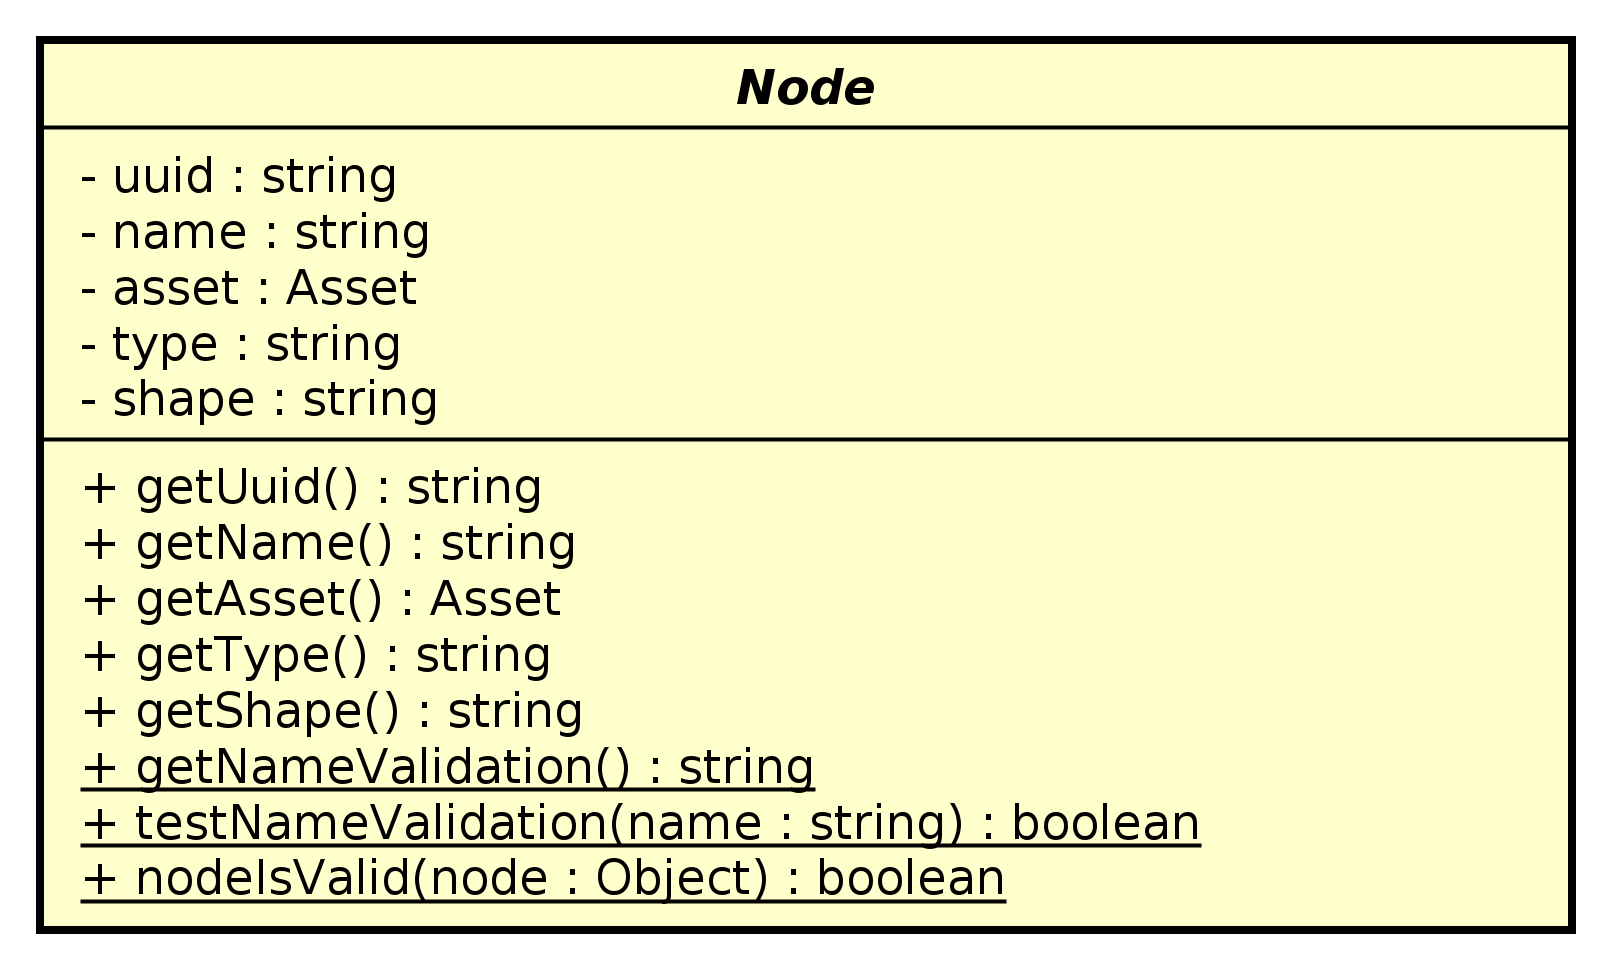
\includegraphics[width=0.3\textwidth]{./img/Node.png}
		\caption{Diagramma classe Node}
	\end{figure}
	\item \textbf{descrizione:} rappresenta un nodo contenuto all'interno di un Asset ;
	\item \textbf{utilizzo:} è contenuto all'interno di Process;
	\item \textbf{attributi:}
	\begin{itemize}
		\item -asset : Asset\begin{itemize}
			\item rappresenta l'asset a cui il nodo appartiene.\end{itemize}
		\item -name : string\begin{itemize}
			\item rappresenta il nome del nodo.\end{itemize}
		\item -shape : string\begin{itemize}
			\item rappresenta la forma del nodo.\end{itemize}
		\item -type : string\begin{itemize}
			\item rappresenta la classe del nodo.\end{itemize}
		\item -uuid : string\begin{itemize}
			\item rappresenta il codice identificativo del nodo (uuid).\end{itemize}
	\end{itemize}
	\item \textbf{metodi:}
	\begin{itemize}
		\item +getAsset() : Asset\newline
		il metodo ritorna l'asset di appartenenza del nodo
		\item +getName() : string\newline
		il metodo ritorna il codice identificativo del nodo
		\item +getNameValidation() : string\newline
		il metodo ritorna l'espressione regolare che indica una stringa non contenente le seguenti caratteristiche: vuota; più
		lunga di 50 caratteri; inizia e/o finisce con uno spazio; contiene caratteri speciali;
		\item +getShape() : string\newline
		il metodo ritorna la forma del nodo
		\item +getType() : string\newline
		il metodo ritorna la classe del nodo
		\item +getUuid() : string\newline
		il metodo ritorna il codice identificativo del nodo (uuid)
		\item +nodeIsValid() : boolean\newline
		il metodo testa che i parametri con cui il nodo sta per essere creato siano validi
		\item +testNameValidation(name) : boolean\newline
		il metodo ritorna true solamente se il valore ricevuto in input, come parametro, è ritenuto valido.
		\begin{itemize}
			\item name : string\\
			rappresenta il nome del nodo.
		\end{itemize}
	\end{itemize}
	\item \textbf{relazioni con altre classi:} 
	\begin{itemize}
		\item IN NodeReducer.
	\end{itemize}
\end{itemize}
\paragraph{Process}
\begin{itemize}
	\begin{figure}[H]
		\centering
		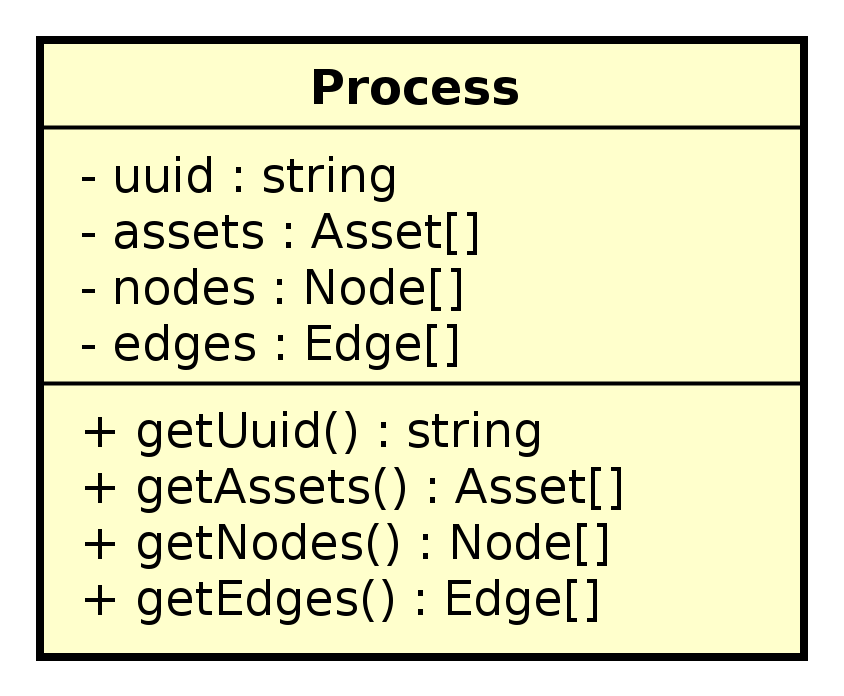
\includegraphics[width=0.3\textwidth]{./img/Process.png}
		\caption{Diagramma classe Process}
	\end{figure}
	\item \textbf{descrizione:} rappresenta un processo produttivo dell'azienda dell'assicurando;
	\item \textbf{utilizzo:} è memorizzato nello Store;
	\item \textbf{attributi:}
	\begin{itemize}
		\item -assets : Asset[ ]\begin{itemize}
			\item rappresenta gli asset facenti parti del processo produttivo.\end{itemize}
		\item -edges : Edge [ ]\begin{itemize}
			\item rappresenta gli archi che effettuano i collegamenti nel processo produttivo.\end{itemize}
		\item -nodes : Node [ ]\begin{itemize}
			\item rappresenta i nodi facenti parti del processo produttivo.\end{itemize}
		\item -uuid : string\begin{itemize}
			\item rappresenta l'identificativo del processo (uuid).\end{itemize}
	\end{itemize}
	\item \textbf{metodi:}
	\begin{itemize}
		\item +getAssets() : Asset[ ]\newline
		il metodo ritorna gli asset facenti parti del processo produttivo
		\item +getEdges() : Edge [ ]\newline
		il metodo ritorna gli archi che effettuano i collegamenti nel processo produttivo
		\item +getNodes() : Node [ ]\newline
		il metodo ritorna i nodi facenti parti del processo produttivo
		\item +getUuid() : string\newline
		il metodo ritorna il codice identificativo (uuid) del processo
	\end{itemize}
\end{itemize}
\paragraph{QueueNode}
\begin{itemize}
	\begin{figure}[H]
		\centering
		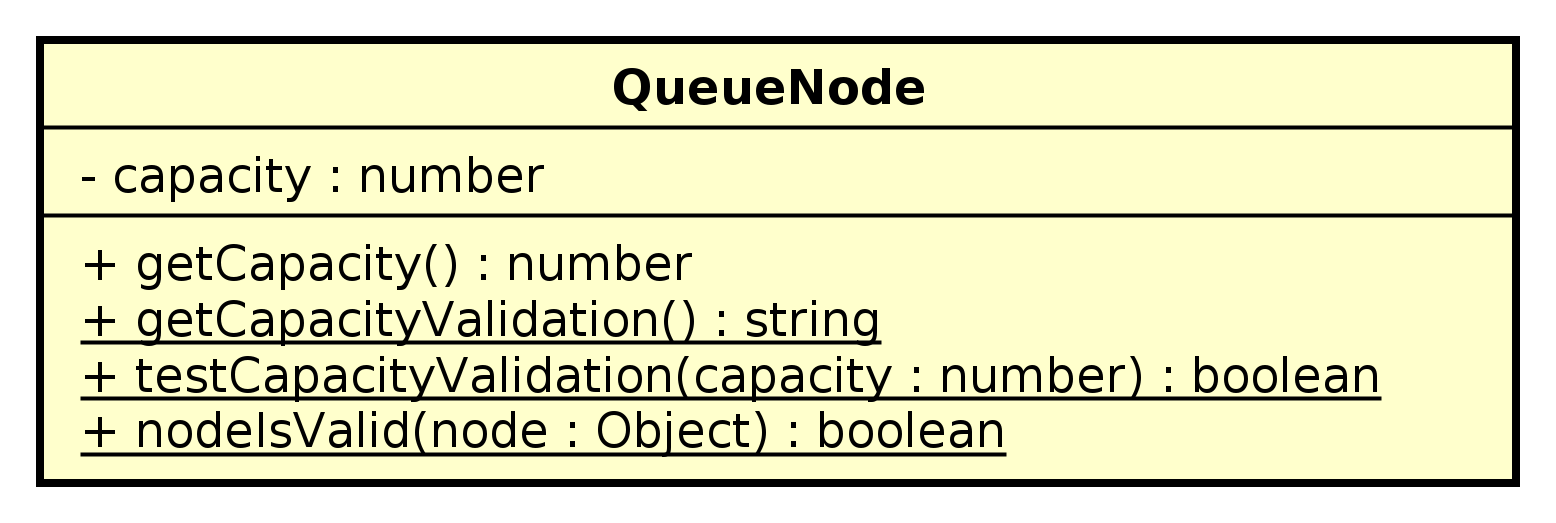
\includegraphics[width=0.3\textwidth]{./img/QueueNode.png}
		\caption{Diagramma classe QueueNode}
	\end{figure}
	\item \textbf{descrizione:} rappresenta un nodo di tipo Coda;
	\item \textbf{utilizzo:} è contenuto all'interno di Process;
	\item \textbf{attributi:}
	\begin{itemize}
		\item -capacity : number\begin{itemize}
			\item rappresenta la capacità del nodo coda.\end{itemize}
	\end{itemize}
	\item \textbf{metodi:}
	\begin{itemize}
		\item +getCapacity() : number\newline
		il metodo ritorna la capacità del nodo
		\item +getCapacityValidation() : string\newline
		il metodo ritorna l'espressione regolare che indica una stringa non contenente le seguenti caratteristiche: vuota; più lunga di 5 cifre per la parte intera; più di 2 per la parte decimale;
		\item +nodeIsValid(node) : boolean\newline
		il metodo testa che i parametri con cui il nodo sta per essere creato siano validi
		\begin{itemize}
			\item node : Object\\
			oggetto che rappresenta i parametri con cui il nodo sta per essere creato.
		\end{itemize}
		\item +testCapacityValidation(capacity) : boolean\newline
		il metodo ritorna true solamente se il valore ricevuto in input, come parametro, è ritenuto valido.
		\begin{itemize}
			\item capacity : number\\
			rappresenta la capacità del nodo.
		\end{itemize}
	\end{itemize}
\end{itemize}
\paragraph{ResourceNode}
\begin{itemize}
	\begin{figure}[H]
		\centering
		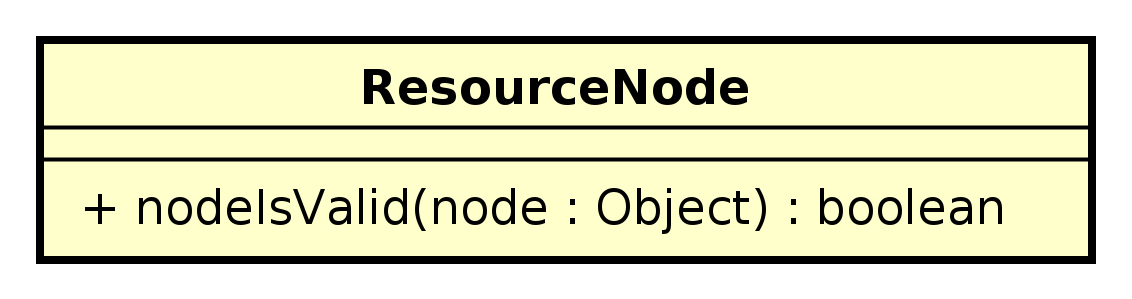
\includegraphics[width=0.3\textwidth]{./img/ResourceNode.png}
		\caption{Diagramma classe ResourceNode}
	\end{figure}
	\item \textbf{descrizione:} rappresenta un nodo di tipo Risorsa;
	\item \textbf{utilizzo:} è contenuto all'interno di Process;
	\item \textbf{metodi:}
	\begin{itemize}
		\item +nodeIsValid() : boolean\newline
		il metodo testa che i parametri con cui il nodo sta per essere creato siano validi
	\end{itemize}
\end{itemize}
\paragraph{SourceNode}
\begin{itemize}
	\begin{figure}[H]
		\centering
		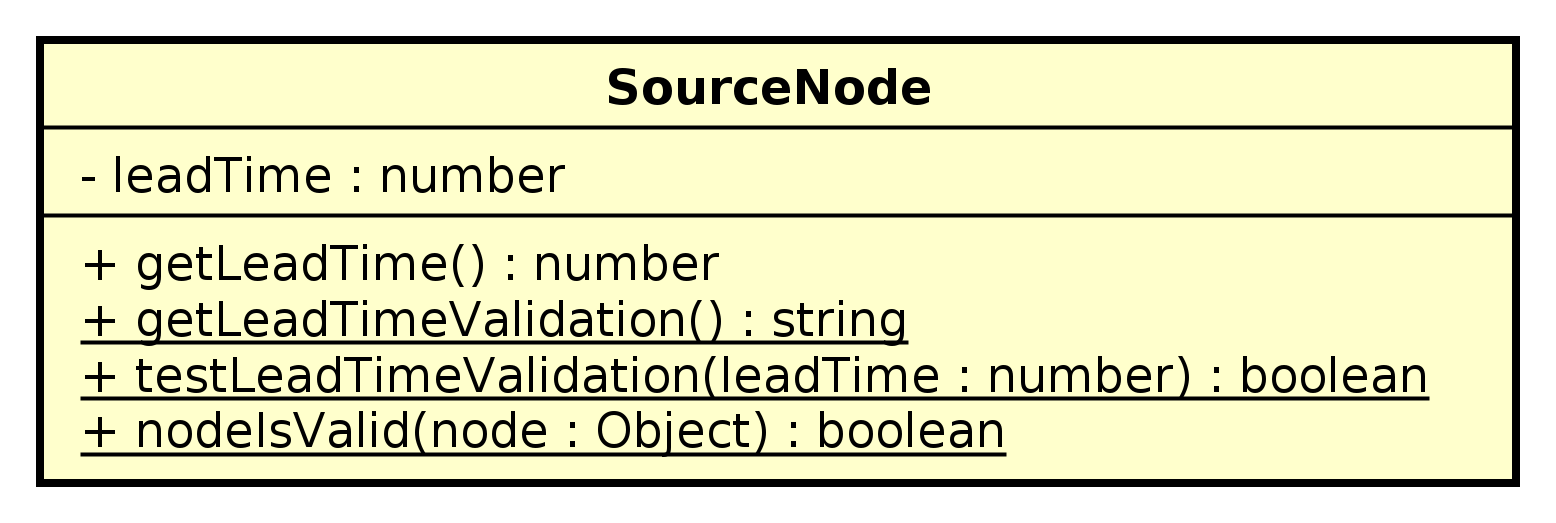
\includegraphics[width=0.3\textwidth]{./img/SourceNode.png}
		\caption{Diagramma classe SourceNode}
	\end{figure}
	\item \textbf{descrizione:} rappresenta un nodo di tipo Sorgente;
	\item \textbf{utilizzo:} è contenuto all'interno di Process;
	\item \textbf{attributi:}
	\begin{itemize}
		\item -leadTime : Object\begin{itemize}
			\item rappresenta il tempo di approvvigionamento del nodo.\end{itemize}
	\end{itemize}
	\item \textbf{metodi:}
	\begin{itemize}
		\item +getLeadTime() : number\newline
		il metodo ritorna il tempo di approvigionamento del nodo
		\item +getLeadTimeValidation() : string\newline
		il metodo ritorna l'espressione regolare che indica una stringa non contenente le seguenti caratteristiche: vuota; più lunga di 5 cifre per la parte intera; più di 2 per la parte decimale;
		\item +nodeIsValid(node) : boolean\newline
		il metodo testa se i parametri con cui il nodo sta per essere creato sono validi
		\begin{itemize}
			\item node : Object\\
			oggetto che rappresenta i parametri con cui il nodo sta per essere creato.
		\end{itemize}
		\item +testLeadTimeValidation(leadTime) : boolean\newline
		il metodo testa se il tempo di approvvigionamento è valido
		\begin{itemize}
			\item leadTime : number\\
			rappresenta il tempo di approvvigionamento.
		\end{itemize}
	\end{itemize}
\end{itemize}
\newpage
\subsection{DeGeOP::StorePkg::PolygonPkg}
\label{pkg::PolygonPkg}
\subsubsection{Informazioni sul package}
\begin{itemize}
	\item \textbf{descrizione:} racchiude le componenti necessarie alla rappresentazione dell'area degli asset e degli scenari di danno;
	\item \textbf{padre:} \hyperref[pkg::StorePkg]{StorePkg};
	\item \textbf{interazioni con altri package:} 
	\begin{itemize}
		\item IN AnalysisPkg: riferimento ad un poligono;
		\item IN ProcessPkg: riferimento ad un poligono.
	\end{itemize}
	\item \textbf{classi contenute:}
	\begin{itemize}
		\item ConcretePolygon;
		\item ConcretePolygonFactory;
		\item Coordinate;
		\item Polygon;
		\item PolygonFactory.
	\end{itemize}
\end{itemize}
\subsubsection{Classi}
\paragraph{ConcretePolygon}
\begin{itemize}
	\begin{figure}[H]
		\centering
		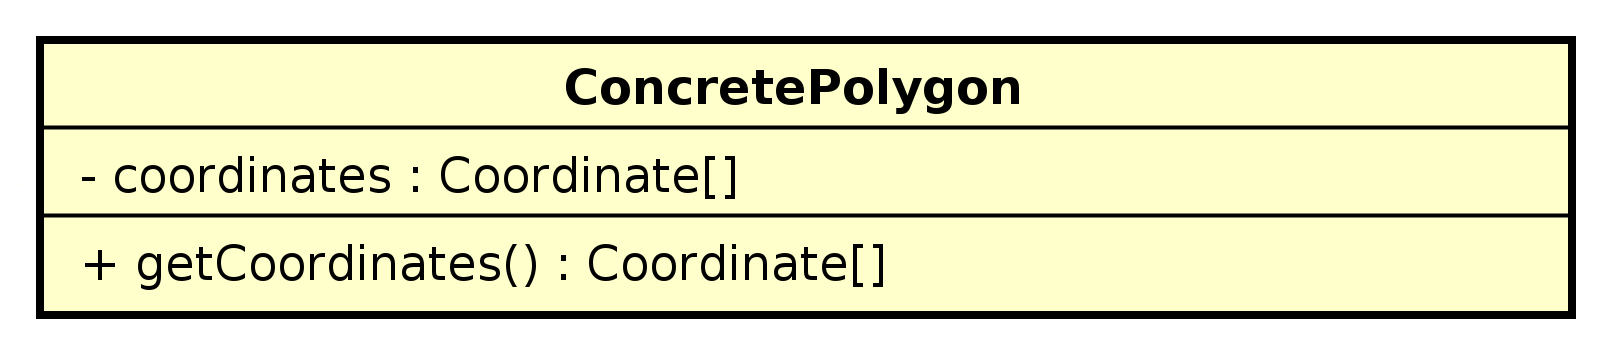
\includegraphics[width=0.3\textwidth]{./img/ConcretePolygon.png}
		\caption{Diagramma classe ConcretePolygon}
	\end{figure}
	\item \textbf{descrizione:} rappresenta un poligono;
	\item \textbf{utilizzo:} viene istanziata da ConcretePolygonFactory; viene utilizzata in Asset e Scenario;
	\item \textbf{attributi:}
	\begin{itemize}
		\item -coordinates : Coordinate[]\begin{itemize}
			\item rappresenta le coordinate che vanno a delineare il poligono.\end{itemize}
	\end{itemize}
	\item \textbf{metodi:}
	\begin{itemize}
		\item +getCoordinates() : Coordinate[]\newline
		il metodo restituisce le coordinate che vanno a delineare il poligono
	\end{itemize}
\end{itemize}
\paragraph{ConcretePolygonFactory}
\begin{itemize}
	\begin{figure}[H]
		\centering
		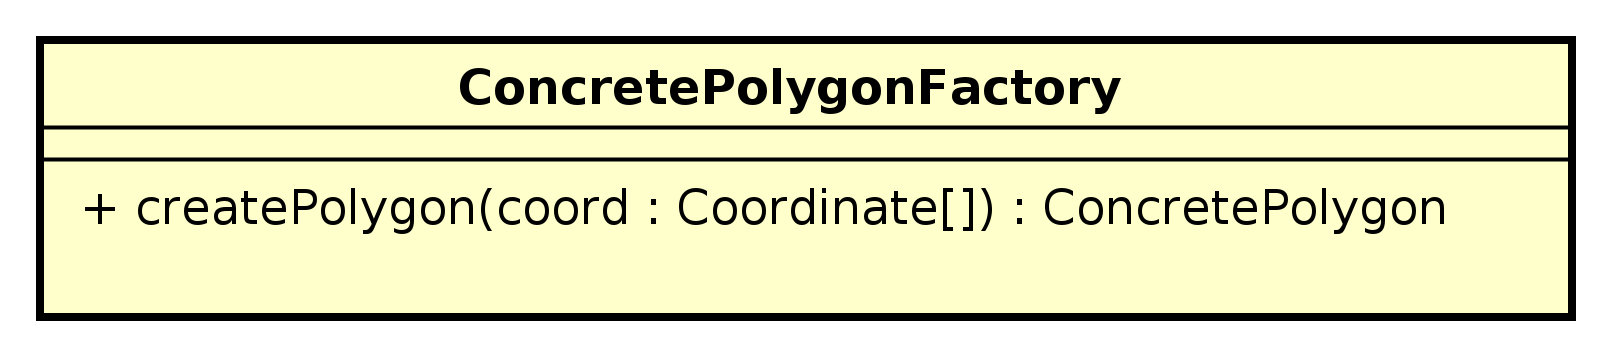
\includegraphics[width=0.3\textwidth]{./img/ConcretePolygonFactory.png}
		\caption{Diagramma classe ConcretePolygonFactory}
	\end{figure}
	\item \textbf{descrizione:} gestisce la creazione concreta dei poligoni;
	\item \textbf{utilizzo:} implementazione di PolygonFactory; è la classe concreta da istanziare per gestire la creazione di un poligono;
	\item \textbf{metodi:}
	\begin{itemize}
		\item +createPolygon() : ConcretePolygon\newline
		il metodo si occupa della costruzione del poligono
	\end{itemize}
\end{itemize}
\paragraph{Coordinate}
\begin{itemize}
	\begin{figure}[H]
		\centering
		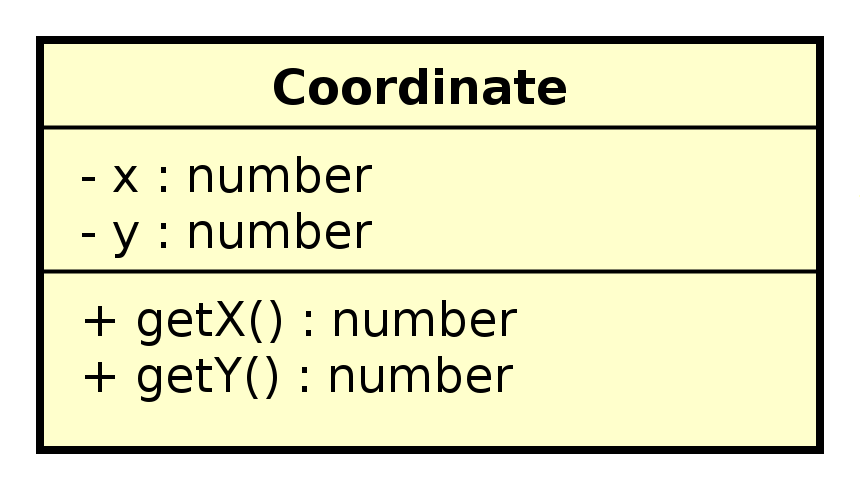
\includegraphics[width=0.3\textwidth]{./img/Coordinate.png}
		\caption{Diagramma classe Coordinate}
	\end{figure}
	\item \textbf{descrizione:} rappresenta una coordinata geografica;
	\item \textbf{utilizzo:} è utilizzata all'interno di Polygon per delimitarne i suoi vertici;
	\item \textbf{attributi:}
	\begin{itemize}
		\item -x : number\begin{itemize}
			\item rappresenta la latitudine di una coordinata geografica.\end{itemize}
		\item -y : number\begin{itemize}
			\item rappresenta la longitudine di una coordinata geografica.\end{itemize}
	\end{itemize}
	\item \textbf{metodi:}
	\begin{itemize}
		\item +getX() : number\newline
		restituisce la latitudine della coordinata geografica
		\item +getY() : number\newline
		restituisce la longitudine della coordinata geografica
	\end{itemize}
\end{itemize}
\paragraph{Polygon}
\begin{itemize}
	\begin{figure}[H]
		\centering
		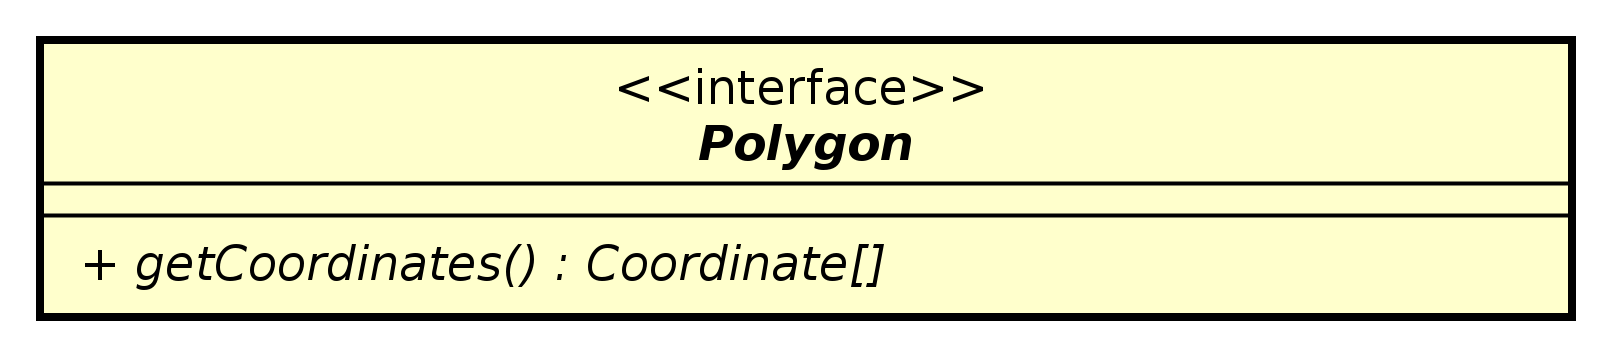
\includegraphics[width=0.3\textwidth]{./img/Polygon.png}
		\caption{Diagramma classe Polygon}
	\end{figure}
	\item \textbf{descrizione:} interfaccia che rappresenta il poligono;
	\item \textbf{utilizzo:} fornisce i metodi del poligono;
	\item \textbf{metodi:}
	\begin{itemize}
		\item +getCoordinates() : Coordinate[]\newline
		il metodo restituisce un array di coordinate
	\end{itemize}
\end{itemize}
\paragraph{PolygonFactory}
\begin{itemize}
	\begin{figure}[H]
		\centering
		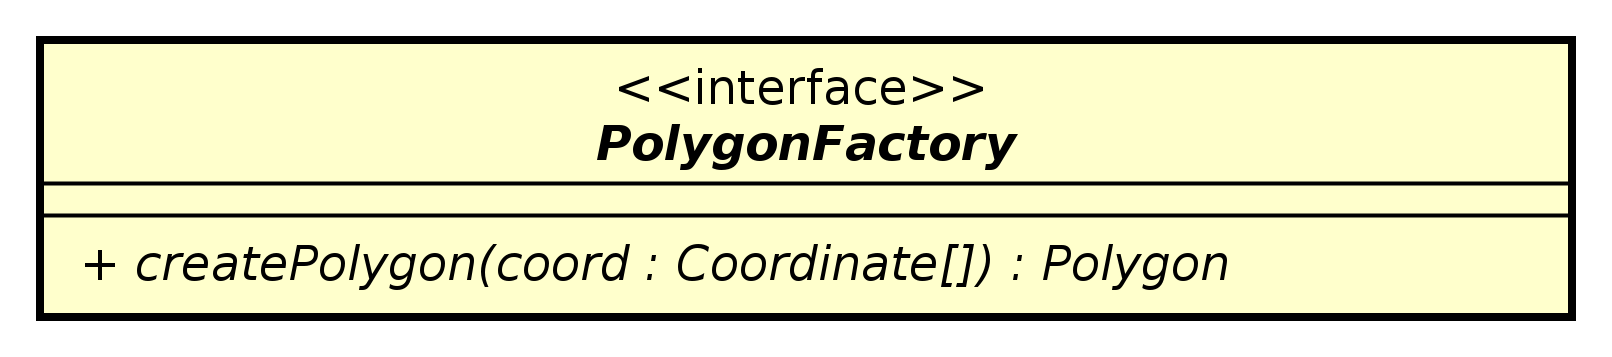
\includegraphics[width=0.3\textwidth]{./img/PolygonFactory.png}
		\caption{Diagramma classe PolygonFactory}
	\end{figure}
	\item \textbf{descrizione:} interfaccia che si occupa della costruzione dei poligoni;
	\item \textbf{utilizzo:} viene usata dalle classi Scenario e Asset per la costruzione dei poligoni;
	\item \textbf{metodi:}
	\begin{itemize}
		\item +createPolygon(coord) : Polygon\newline
		il metodo si occupa della costruzione del poligono
		\begin{itemize}
			\item coord : Coordinate[]\\
			raccoglie le coordinate necessarie alla costruzione dei poligoni
			.
		\end{itemize}
	\end{itemize}
\end{itemize}
\newpage
\subsection{DeGeOP::ReducerPkg}
\label{pkg::ReducerPkg}
\begin{figure}[H]
	\centering
	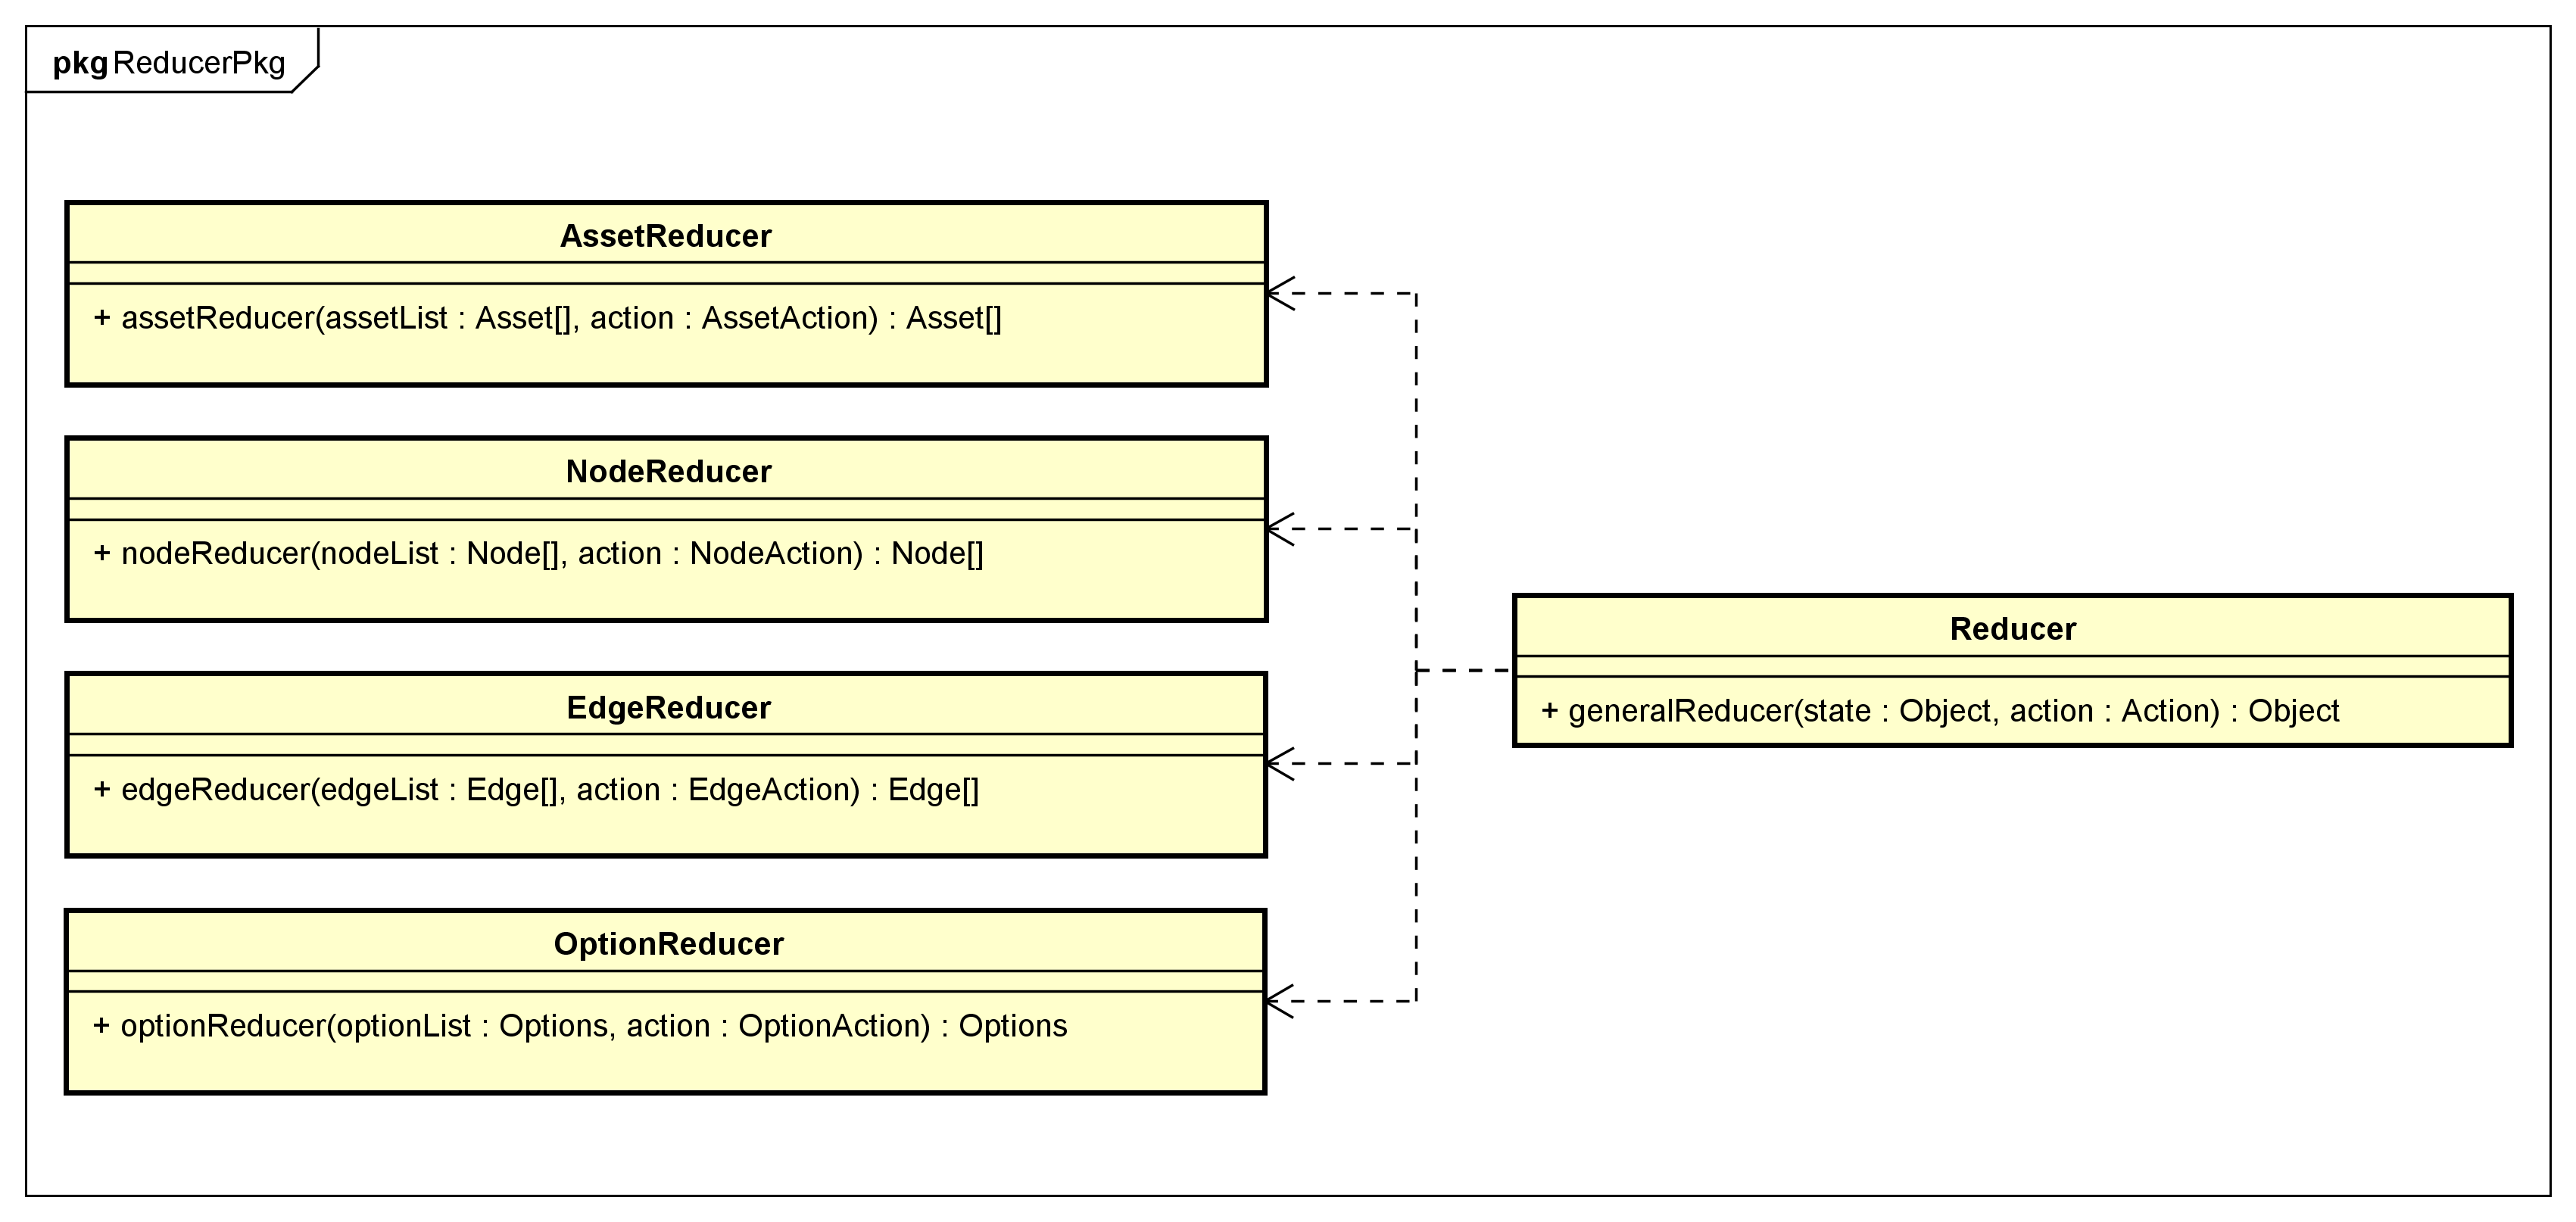
\includegraphics[width=\textwidth]{img/PkgDiagram/ReducerPkg.png}
	\caption{Schema componente DeGeOP::ReducerPkg}
\end{figure}
\subsubsection{Informazioni sul package}
\begin{itemize}
	\item \textbf{descrizione:} racchiude le componenti necessarie all'implementazione dei reducer secondo l'architettura Redux;
	\item \textbf{padre:} \hyperref[pkg::DeGeOP]{DeGeOP};
	\item \textbf{interazioni con altri package:} 
	\begin{itemize}
		\item OUT ActionPkg: utilizzo di azioni ;
		\item OUT StorePkg: applicazione di cambiamenti di stato.
	\end{itemize}
	\item \textbf{classi contenute:}
	\begin{itemize}
		\item AssetReducer;
		\item EdgeReducer;
		\item NodeReducer;
		\item OptionReducer;
		\item Reducer.
	\end{itemize}
\end{itemize}
\subsubsection{Classi}
\paragraph{AssetReducer}
\begin{itemize}
	\begin{figure}[H]
		\centering
		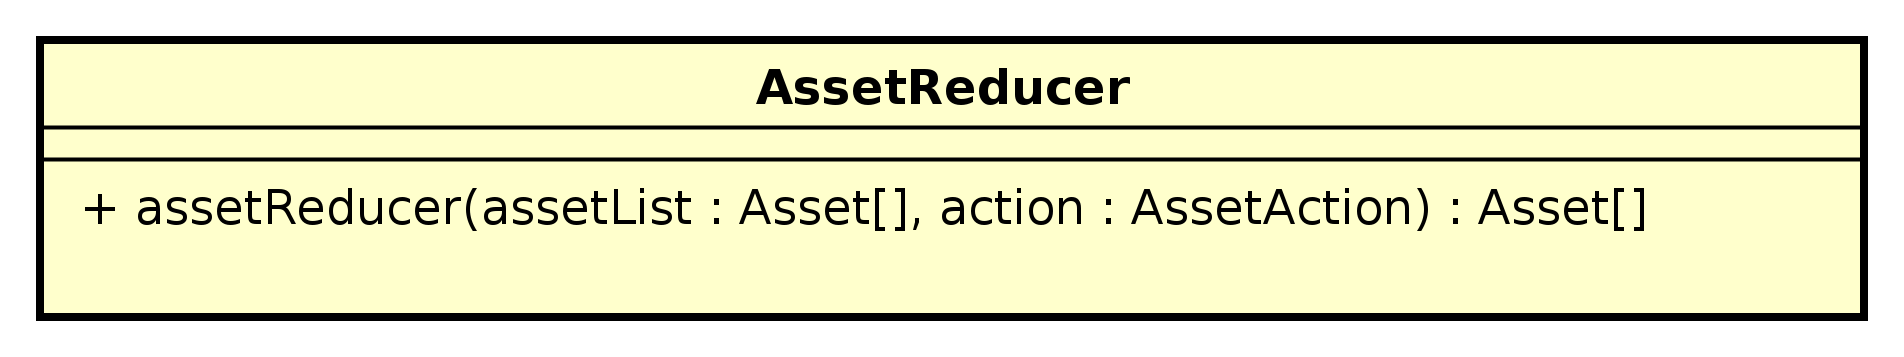
\includegraphics[width=0.3\textwidth]{./img/AssetReducer.png}
		\caption{Diagramma classe AssetReducer}
	\end{figure}
	\item \textbf{descrizione:} rappresenta il reducer dell'asset;
	\item \textbf{utilizzo:} il suo metodo gestisce le operazioni sullo store riguardanti l'asset;
	\item \textbf{metodi:}
	\begin{itemize}
		\item +assetReducer(action, assetList) : Asset[ ]\newline
		il metodo gestisce le operazioni sullo store riguardanti l'asset e ritorna la nuova lista di asset ottenuta a seguito della modifica
		\begin{itemize}
			\item action : AssetAction\\
			rappresenta un'azione che descrive i cambiamenti da effettuare sullo stato.
			\item assetList : Asset[ ]\\
			rappresenta una lista di asset, che sono il vecchio stato.
		\end{itemize}
	\end{itemize}
	\item \textbf{relazioni con altre classi:} 
	\begin{itemize}
		\item OUT Asset.
	\end{itemize}
\end{itemize}
\paragraph{EdgeReducer}
\begin{itemize}
	\begin{figure}[H]
		\centering
		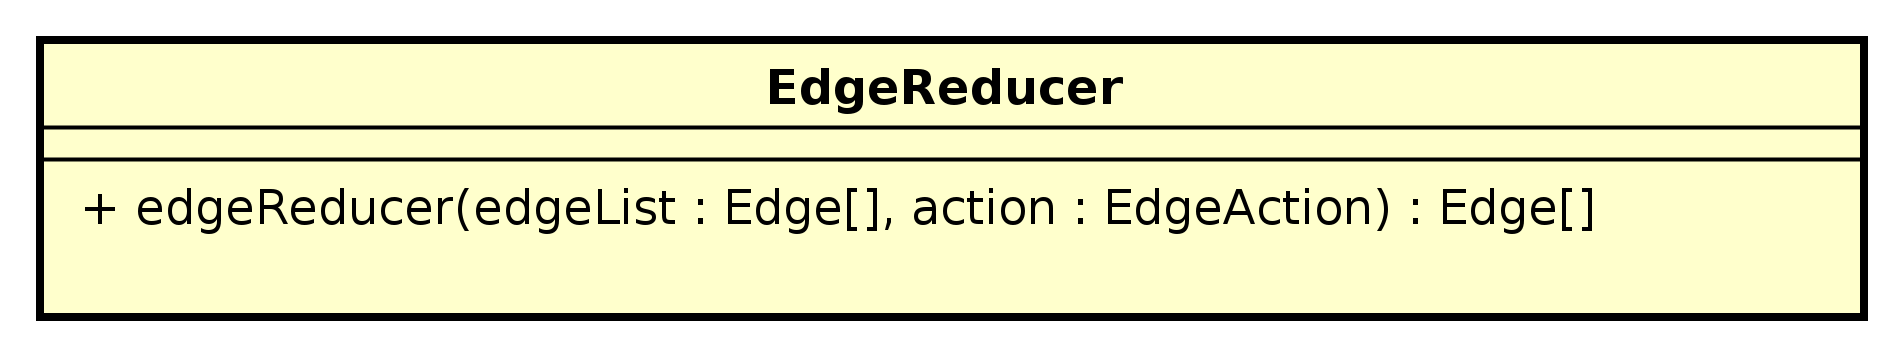
\includegraphics[width=0.3\textwidth]{./img/EdgeReducer.png}
		\caption{Diagramma classe EdgeReducer}
	\end{figure}
	\item \textbf{descrizione:} rappresenta il reducer dell'arco;
	\item \textbf{utilizzo:} il suo metodo gestisce le operazioni sullo store riguardanti gli archi;
	\item \textbf{metodi:}
	\begin{itemize}
		\item +edgeReducer(action, edgeList) : Edge [ ]\newline
		il metodo gestisce le operazioni sullo store riguardanti gli archi e ritorna la nuova lista di archi ottenuta a seguito della modifica
		\begin{itemize}
			\item action : EdgeAction\\
			rappresenta un'azione che descrive i cambiamenti da effettuare sullo stato.
			\item edgeList : Edge [ ]\\
			rappresenta una lista di archi, che sono il vecchio stato.
		\end{itemize}
	\end{itemize}
	\item \textbf{relazioni con altre classi:} 
	\begin{itemize}
		\item OUT Edge.
	\end{itemize}
\end{itemize}
\paragraph{NodeReducer}
\begin{itemize}
	\begin{figure}[H]
		\centering
		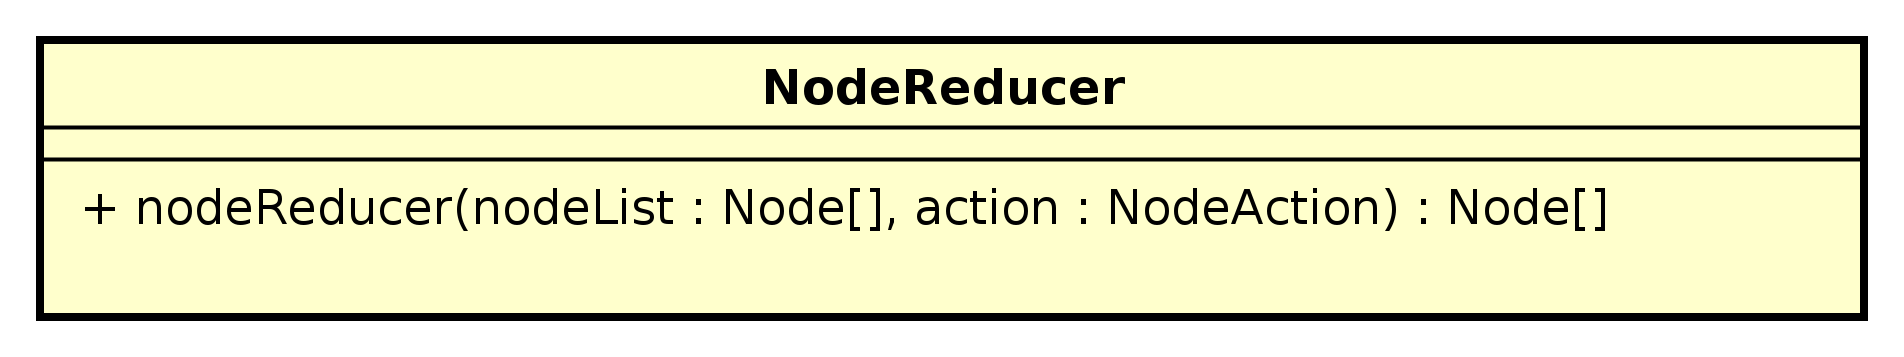
\includegraphics[width=0.3\textwidth]{./img/NodeReducer.png}
		\caption{Diagramma classe NodeReducer}
	\end{figure}
	\item \textbf{descrizione:} rappresenta il reducer del nodo;
	\item \textbf{utilizzo:} il suo metodo gestisce le operazioni sullo store riguardanti i nodi;
	\item \textbf{metodi:}
	\begin{itemize}
		\item +nodeReducer(action, nodeList) : Node [ ]\newline
		il metodo gestisce le operazioni sullo store riguardanti i nodi e ritorna la nuova lista di nodi ottenuta a seguito della modifica
		\begin{itemize}
			\item action : EdgeAction\\
			rappresenta un'azione che descrive i cambiamenti da effettuare sullo stato.
			\item nodeList : Node [ ]\\
			rappresenta una lista di nodi, che sono il vecchio stato.
		\end{itemize}
	\end{itemize}
	\item \textbf{relazioni con altre classi:} 
	\begin{itemize}
		\item OUT Node.
	\end{itemize}
\end{itemize}
\paragraph{OptionReducer}
\begin{itemize}
	\begin{figure}[H]
		\centering
		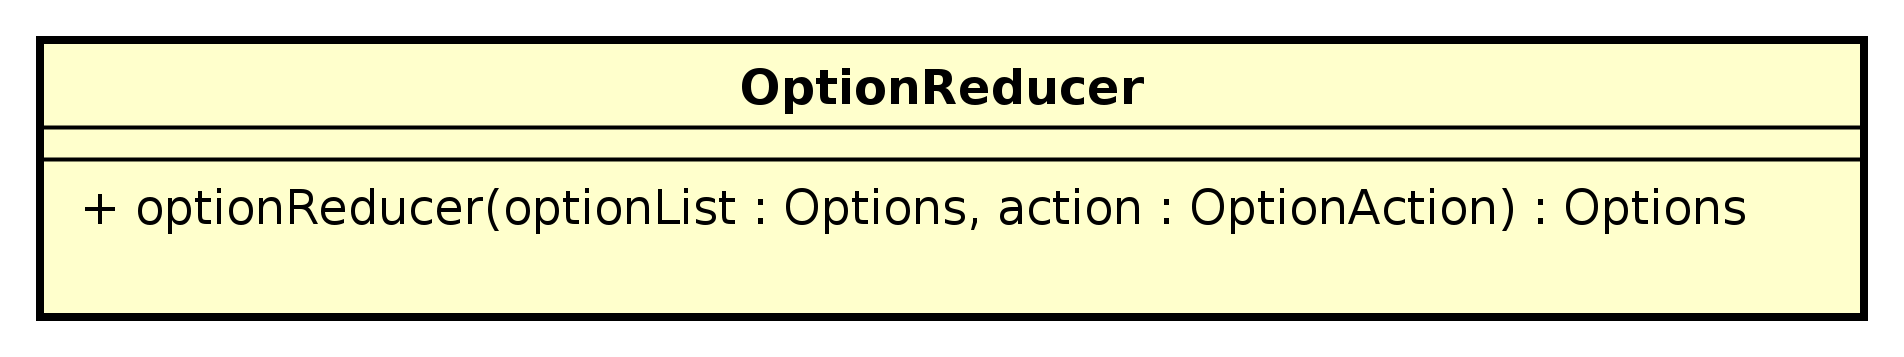
\includegraphics[width=0.3\textwidth]{./img/OptionReducer.png}
		\caption{Diagramma classe OptionReducer}
	\end{figure}
	\item \textbf{descrizione:} rappresenta il reducer delle option;
	\item \textbf{utilizzo:} il suo metodo gestisce le operazioni sullo store riguardanti l'asset;
	\item \textbf{metodi:}
	\begin{itemize}
		\item +optionReducer(action, optionList) : Options\newline
		il metodo gestisce le operazioni sullo store riguardanti l'asset e ritorna la nuova lista di asset ottenuta a seguito della modifica
		\begin{itemize}
			\item action : OptionAction\\
			rappresenta un'azione che descrive i cambiamenti da effettuare sullo stato.
			\item optionList : Options\\
			rappresenta la lista delle option.
		\end{itemize}
	\end{itemize}
	\item \textbf{relazioni con altre classi:} 
	\begin{itemize}
		\item IN Reducer;
		\item OUT Options.
	\end{itemize}
\end{itemize}
\paragraph{Reducer}
\begin{itemize}
	\begin{figure}[H]
		\centering
		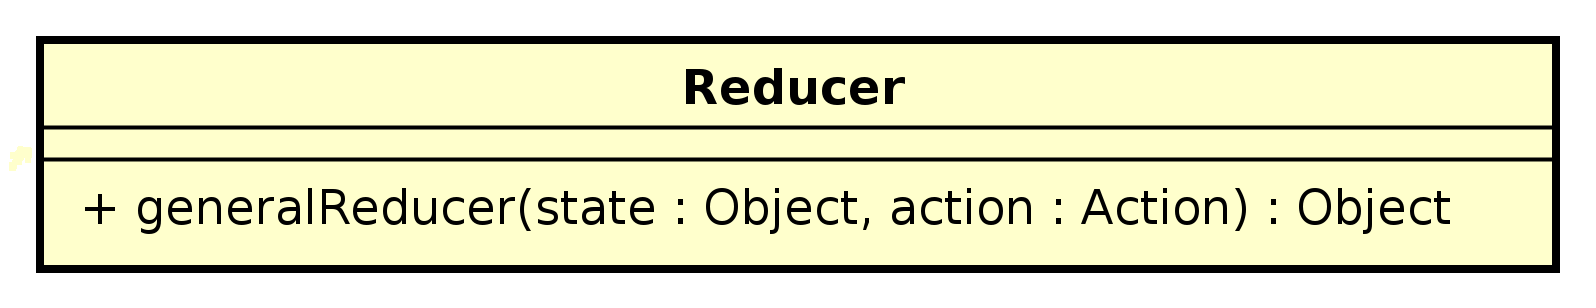
\includegraphics[width=0.3\textwidth]{./img/Reducer.png}
		\caption{Diagramma classe Reducer}
	\end{figure}
	\item \textbf{descrizione:} accetta una action generica in input e la reindirizza al giusto reducer;
	\item \textbf{utilizzo:} il suo metodo viene utilizzato per catturare un'azione e generare un nuovo stato sullo Store;
	\item \textbf{metodi:}
	\begin{itemize}
		\item +generalReducer() : Object\newline
		Esegue l'azione sullo stato corrente dello store e ne ritorna il nuovo stato
	\end{itemize}
	\item \textbf{relazioni con altre classi:} 
	\begin{itemize}
		\item OUT OptionReducer;
		\item OUT StoreDeGeOP.
	\end{itemize}
\end{itemize}
\newpage
\subsection{DeGeOP::CallManagerPkg}
\label{pkg::CallManagerPkg}
\begin{figure}[H]
	\centering
	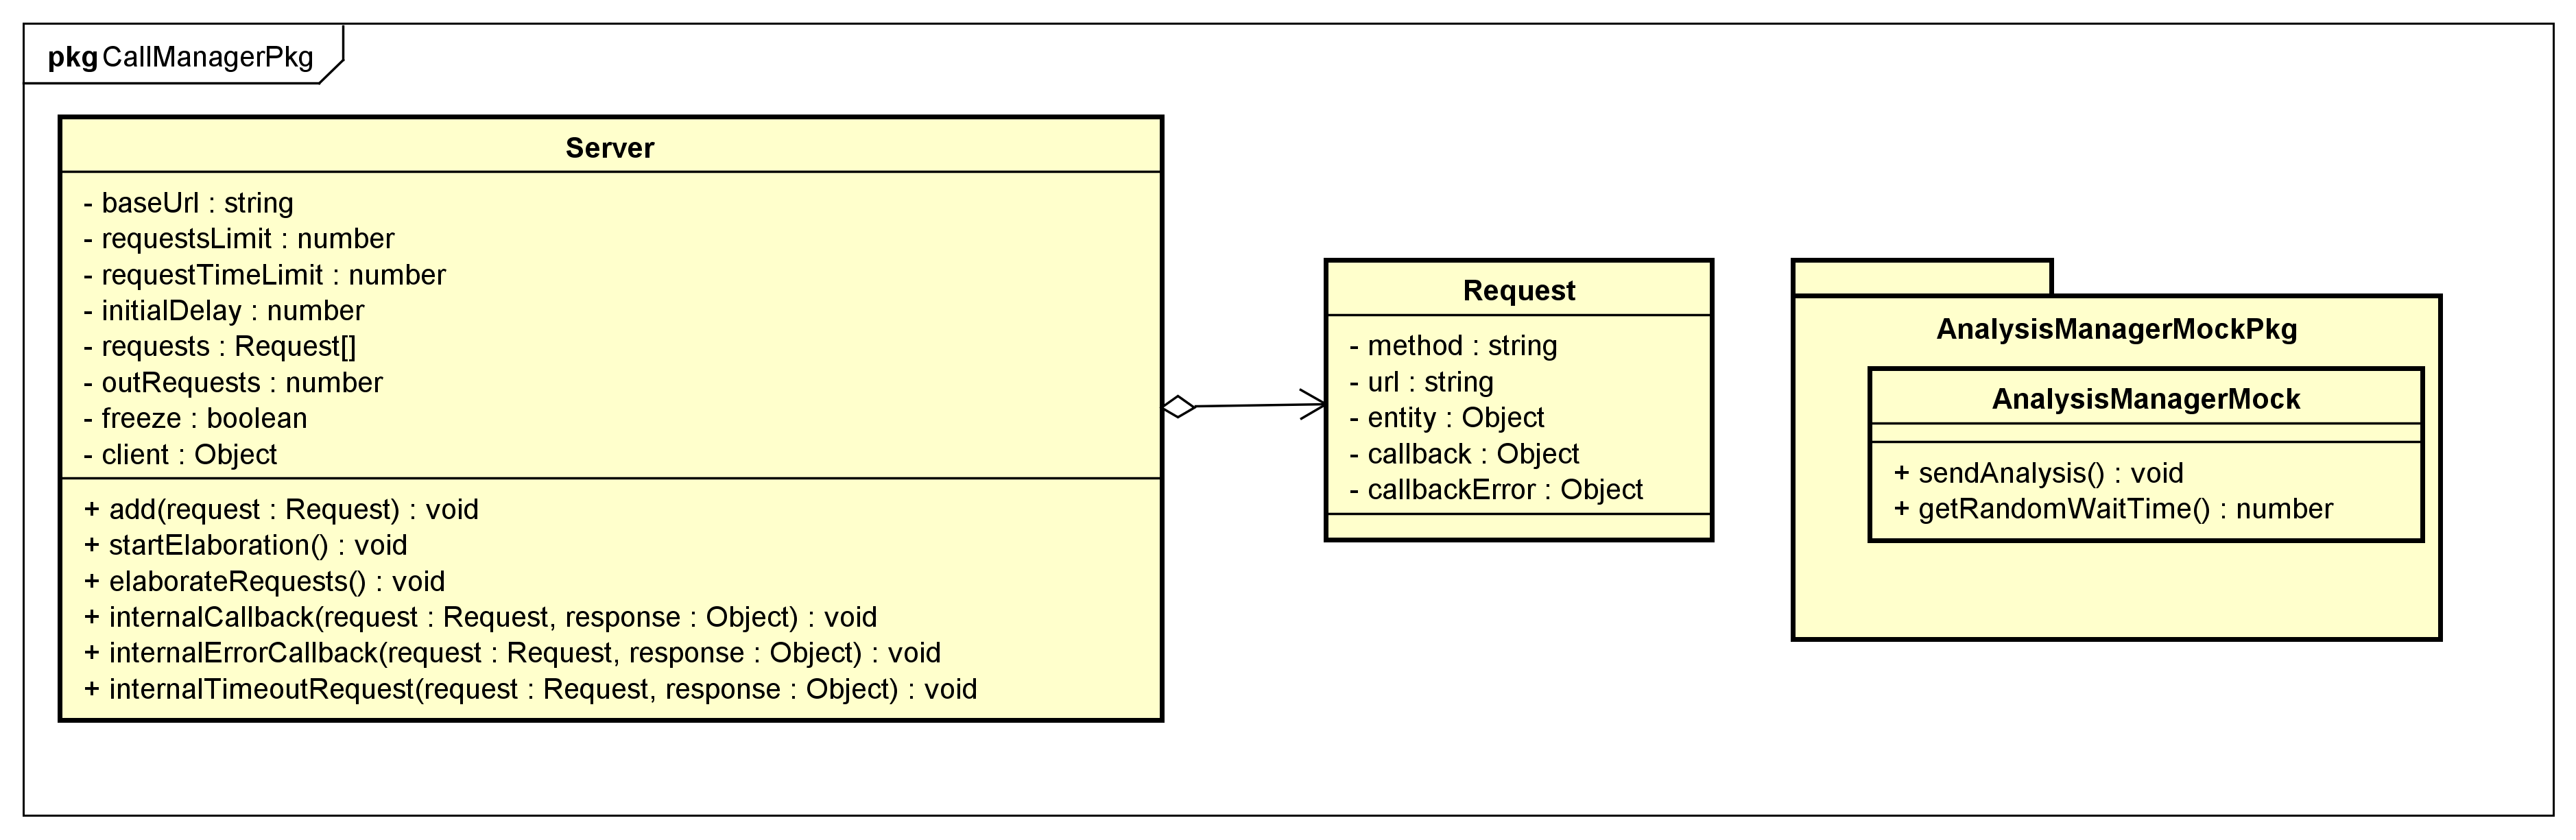
\includegraphics[width=\textwidth]{img/PkgDiagram/CallManagerPkg.png}
	\caption{Schema componente DeGeOP::CallManagerPkg}
\end{figure}
\subsubsection{Informazioni sul package}
\begin{itemize}
	\item \textbf{descrizione:} racchiude le componenti necessarie alla comunicazione dei dati verso il server;
	\item \textbf{padre:} \hyperref[pkg::DeGeOP]{DeGeOP};
	\item \textbf{package contenuti:}
	\begin{itemize}
		\item CallManagerPkg::\hyperref[pkg::AnalysisManagerMockPkg]{AnalysisManagerMockPkg}.
	\end{itemize}
	\item \textbf{interazioni con altri package:} 
	\begin{itemize}
		\item OUT ActionPkg: dispatch di azioni;
		\item OUT StorePkg: subscribe sullo store.
	\end{itemize}
	\item \textbf{classi contenute:}
	\begin{itemize}
		\item Request;
		\item Server.
	\end{itemize}
\end{itemize}
\subsubsection{Classi}
\paragraph{Request}
\begin{itemize}
	\begin{figure}[H]
		\centering
		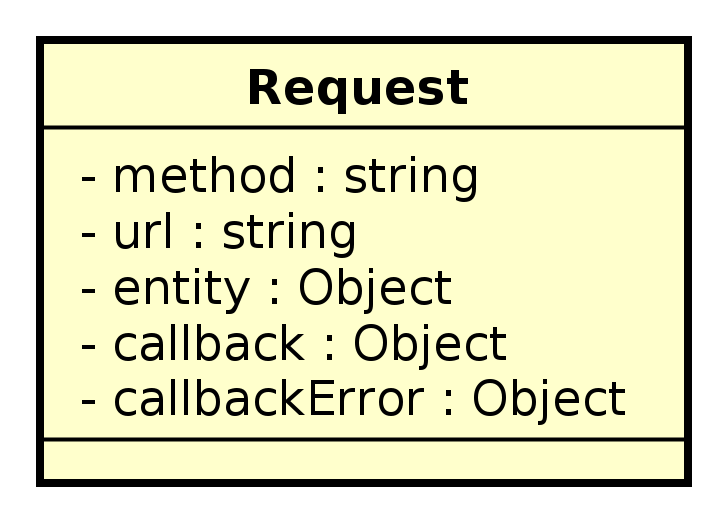
\includegraphics[width=0.3\textwidth]{./img/Request.png}
		\caption{Diagramma classe Request}
	\end{figure}
	\item \textbf{descrizione:} rappresenta i dati necessari per eseguire una richiesta di tipologia REST;
	\item \textbf{utilizzo:} è utilizzata all'interno di Server per gestire la coda delle richieste ;
	\item \textbf{attributi:}
	\begin{itemize}
		\item -callback : Object\begin{itemize}
			\item rappresenta la funzione che viene invocata se la richiesta è andata a buon fine.\end{itemize}
		\item -callbackError : Object\begin{itemize}
			\item rappresenta la funzione che viene invocata se la richiesta non è andata a buon fine.\end{itemize}
		\item -entity : Object\begin{itemize}
			\item rappresnta il payload della richiesta.\end{itemize}
		\item -method : string\begin{itemize}
			\item rappresenta il verbo http con cui si esegue la richiesta.\end{itemize}
		\item -url : string\begin{itemize}
			\item rappresenta l'url verso cui eseguire la richiesta.\end{itemize}
	\end{itemize}
\end{itemize}
\paragraph{Server}
\begin{itemize}
	\begin{figure}[H]
		\centering
		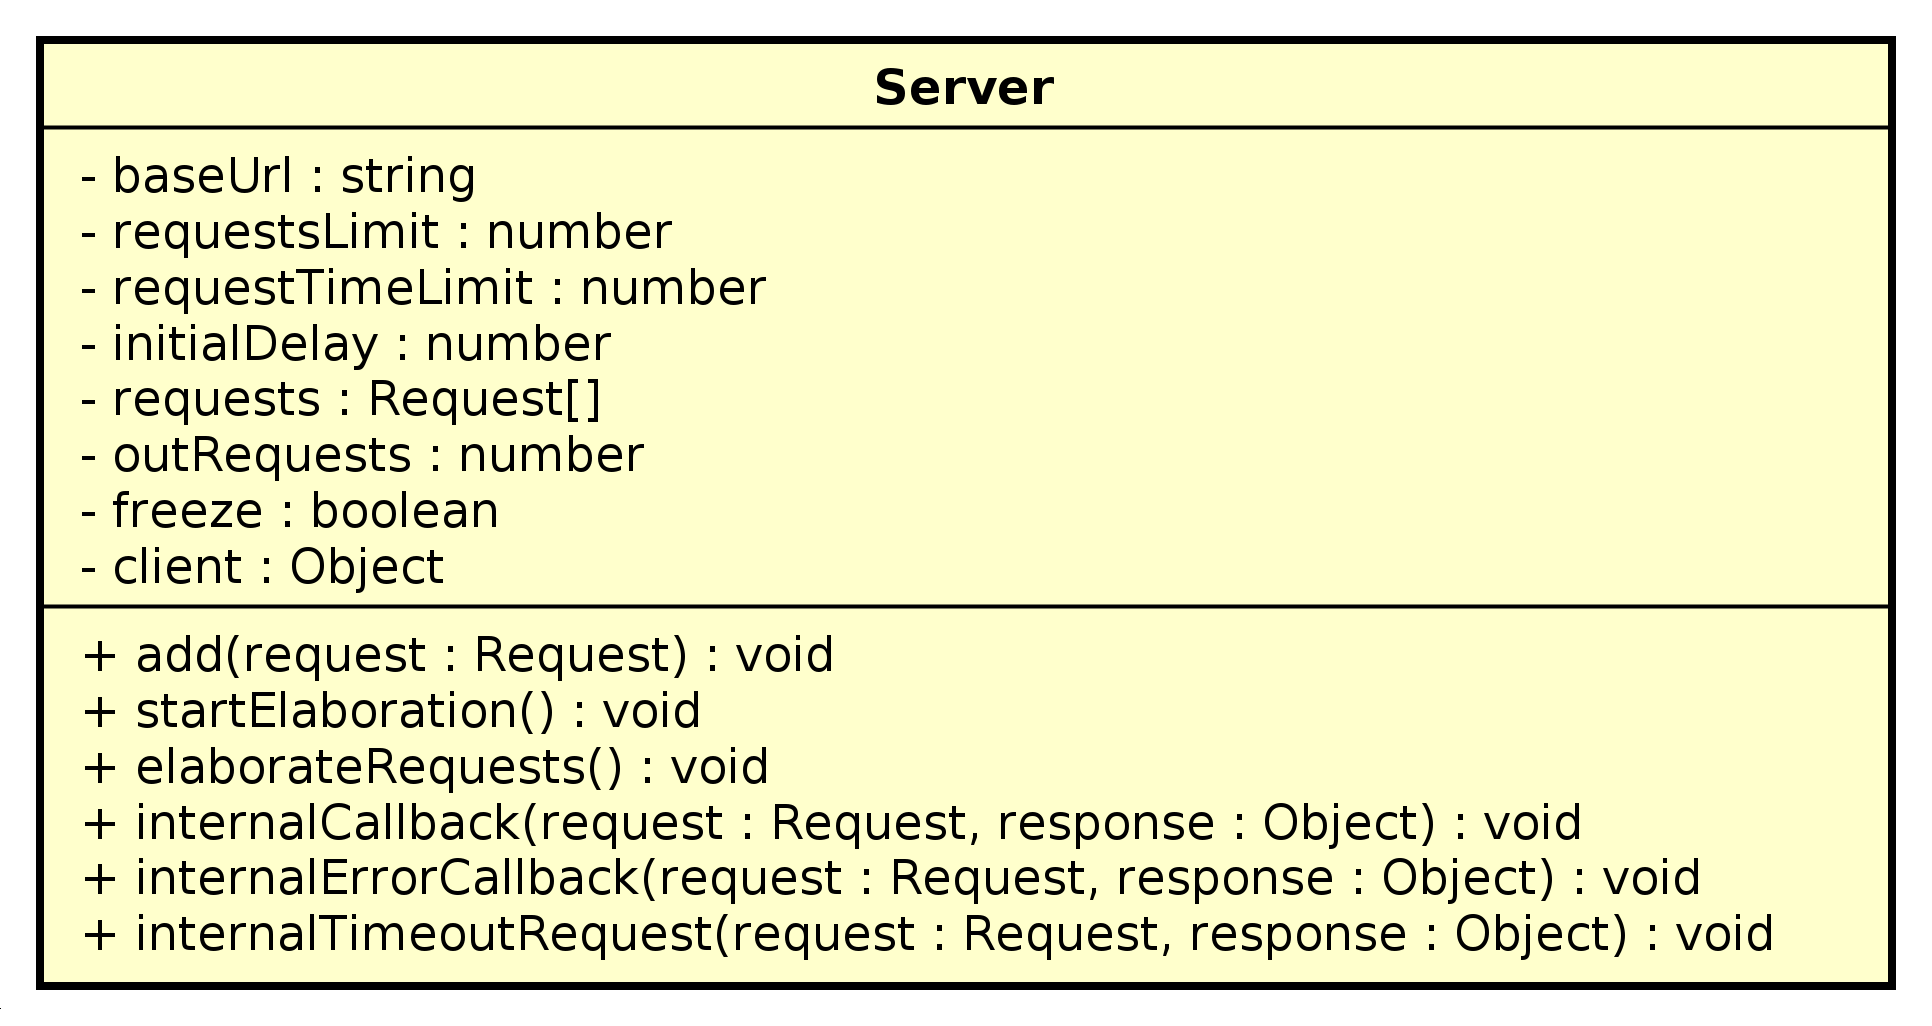
\includegraphics[width=0.3\textwidth]{./img/Server.png}
		\caption{Diagramma classe Server}
	\end{figure}
	\item \textbf{descrizione:} rappresenta il gestore delle chiamate REST;
	\item \textbf{utilizzo:} è utilizzato come buffer per gestire le richieste in uscita e le risposte ricevute;
	\item \textbf{attributi:}
	\begin{itemize}
		\item -baseUrl : string\begin{itemize}
			\item URL http verso cui devono essere inviate le richieste.\end{itemize}
		\item -client : Object\begin{itemize}
			\item gestisce l'invio delle richieste e la ricezione delle risposte.\end{itemize}
		\item -freeze : boolean\begin{itemize}
			\item viene utilizzata per bloccare il server in caso di collegamento mancante.\end{itemize}
		\item -initialDelay : number\begin{itemize}
			\item rappresenta il tempo in millisecondi passato il quale una richiesta scaduta viene eseguita nuovamente.\end{itemize}
		\item -outRequests : number\begin{itemize}
			\item rappresenta il numero delle richieste attualmente in attesa di risposta.\end{itemize}
		\item -requests : Request[]\begin{itemize}
			\item lista delle richieste da evadere.\end{itemize}
		\item -requestsLimit : number\begin{itemize}
			\item rappresenta il numero massimo di richieste eseguite ancora in attesa di risposta.\end{itemize}
		\item -timeLimitRequest : number\begin{itemize}
			\item rappresenta il tempo in millisecondi dopo cui considerare la richiesta scaduta.\end{itemize}
	\end{itemize}
	\item \textbf{metodi:}
	\begin{itemize}
		\item +add(request) : void\newline
		aggiunge una richiesta alla coda del server
		\begin{itemize}
			\item request : Request\\
			rappresenta la richiesta da aggiungere alla coda server.
		\end{itemize}
		\item +elaborateRequests() : void\newline
		elabora la coda della richieste fino a quando ci sono elementi presenti
		\item +internalCallback(request, response) : void\newline
		esegue la chiamata alla funzione di callback fornita dalla richiesta nel caso in cui questa abbia ricevuto una risposta senza errori
		\begin{itemize}
			\item request : Request\\
			rappresenta la richiesta che è stata inviata.
			\item response : Object\\
			oggetto che rappresenta la risposta alla richiesta inviata.
		\end{itemize}
		\item +internalErrorCallback(request, response) : void\newline
		esegue la chiamata alla funzione di callback fornita dalla richiesta nel caso in cui questa abbia ricevuto una risposta con errori
		\begin{itemize}
			\item request : Request\\
			rappresenta la richiesta che è stata inviata.
			\item response : Object\\
			oggetto che rappresenta la risposta alla richiesta inviata.
		\end{itemize}
		\item +internalTimeoutRequest(response) : void\newline
		gestisce la richiesta nel caso in cui questa abbia non abbia ricevuto alcuna risposta entro il tempo di timeout
		\begin{itemize}
			\item response : Object\\
			oggetto che rappresenta la risposta alla richiesta inviata.
		\end{itemize}
		\item +startElaboration() : void\newline
		inizia l'esecuzione delle richieste in attesa di essere evase
	\end{itemize}
\end{itemize}
\newpage
\subsection{DeGeOP::ActionPkg}
\label{pkg::ActionPkg}
\begin{figure}[H]
	\centering
	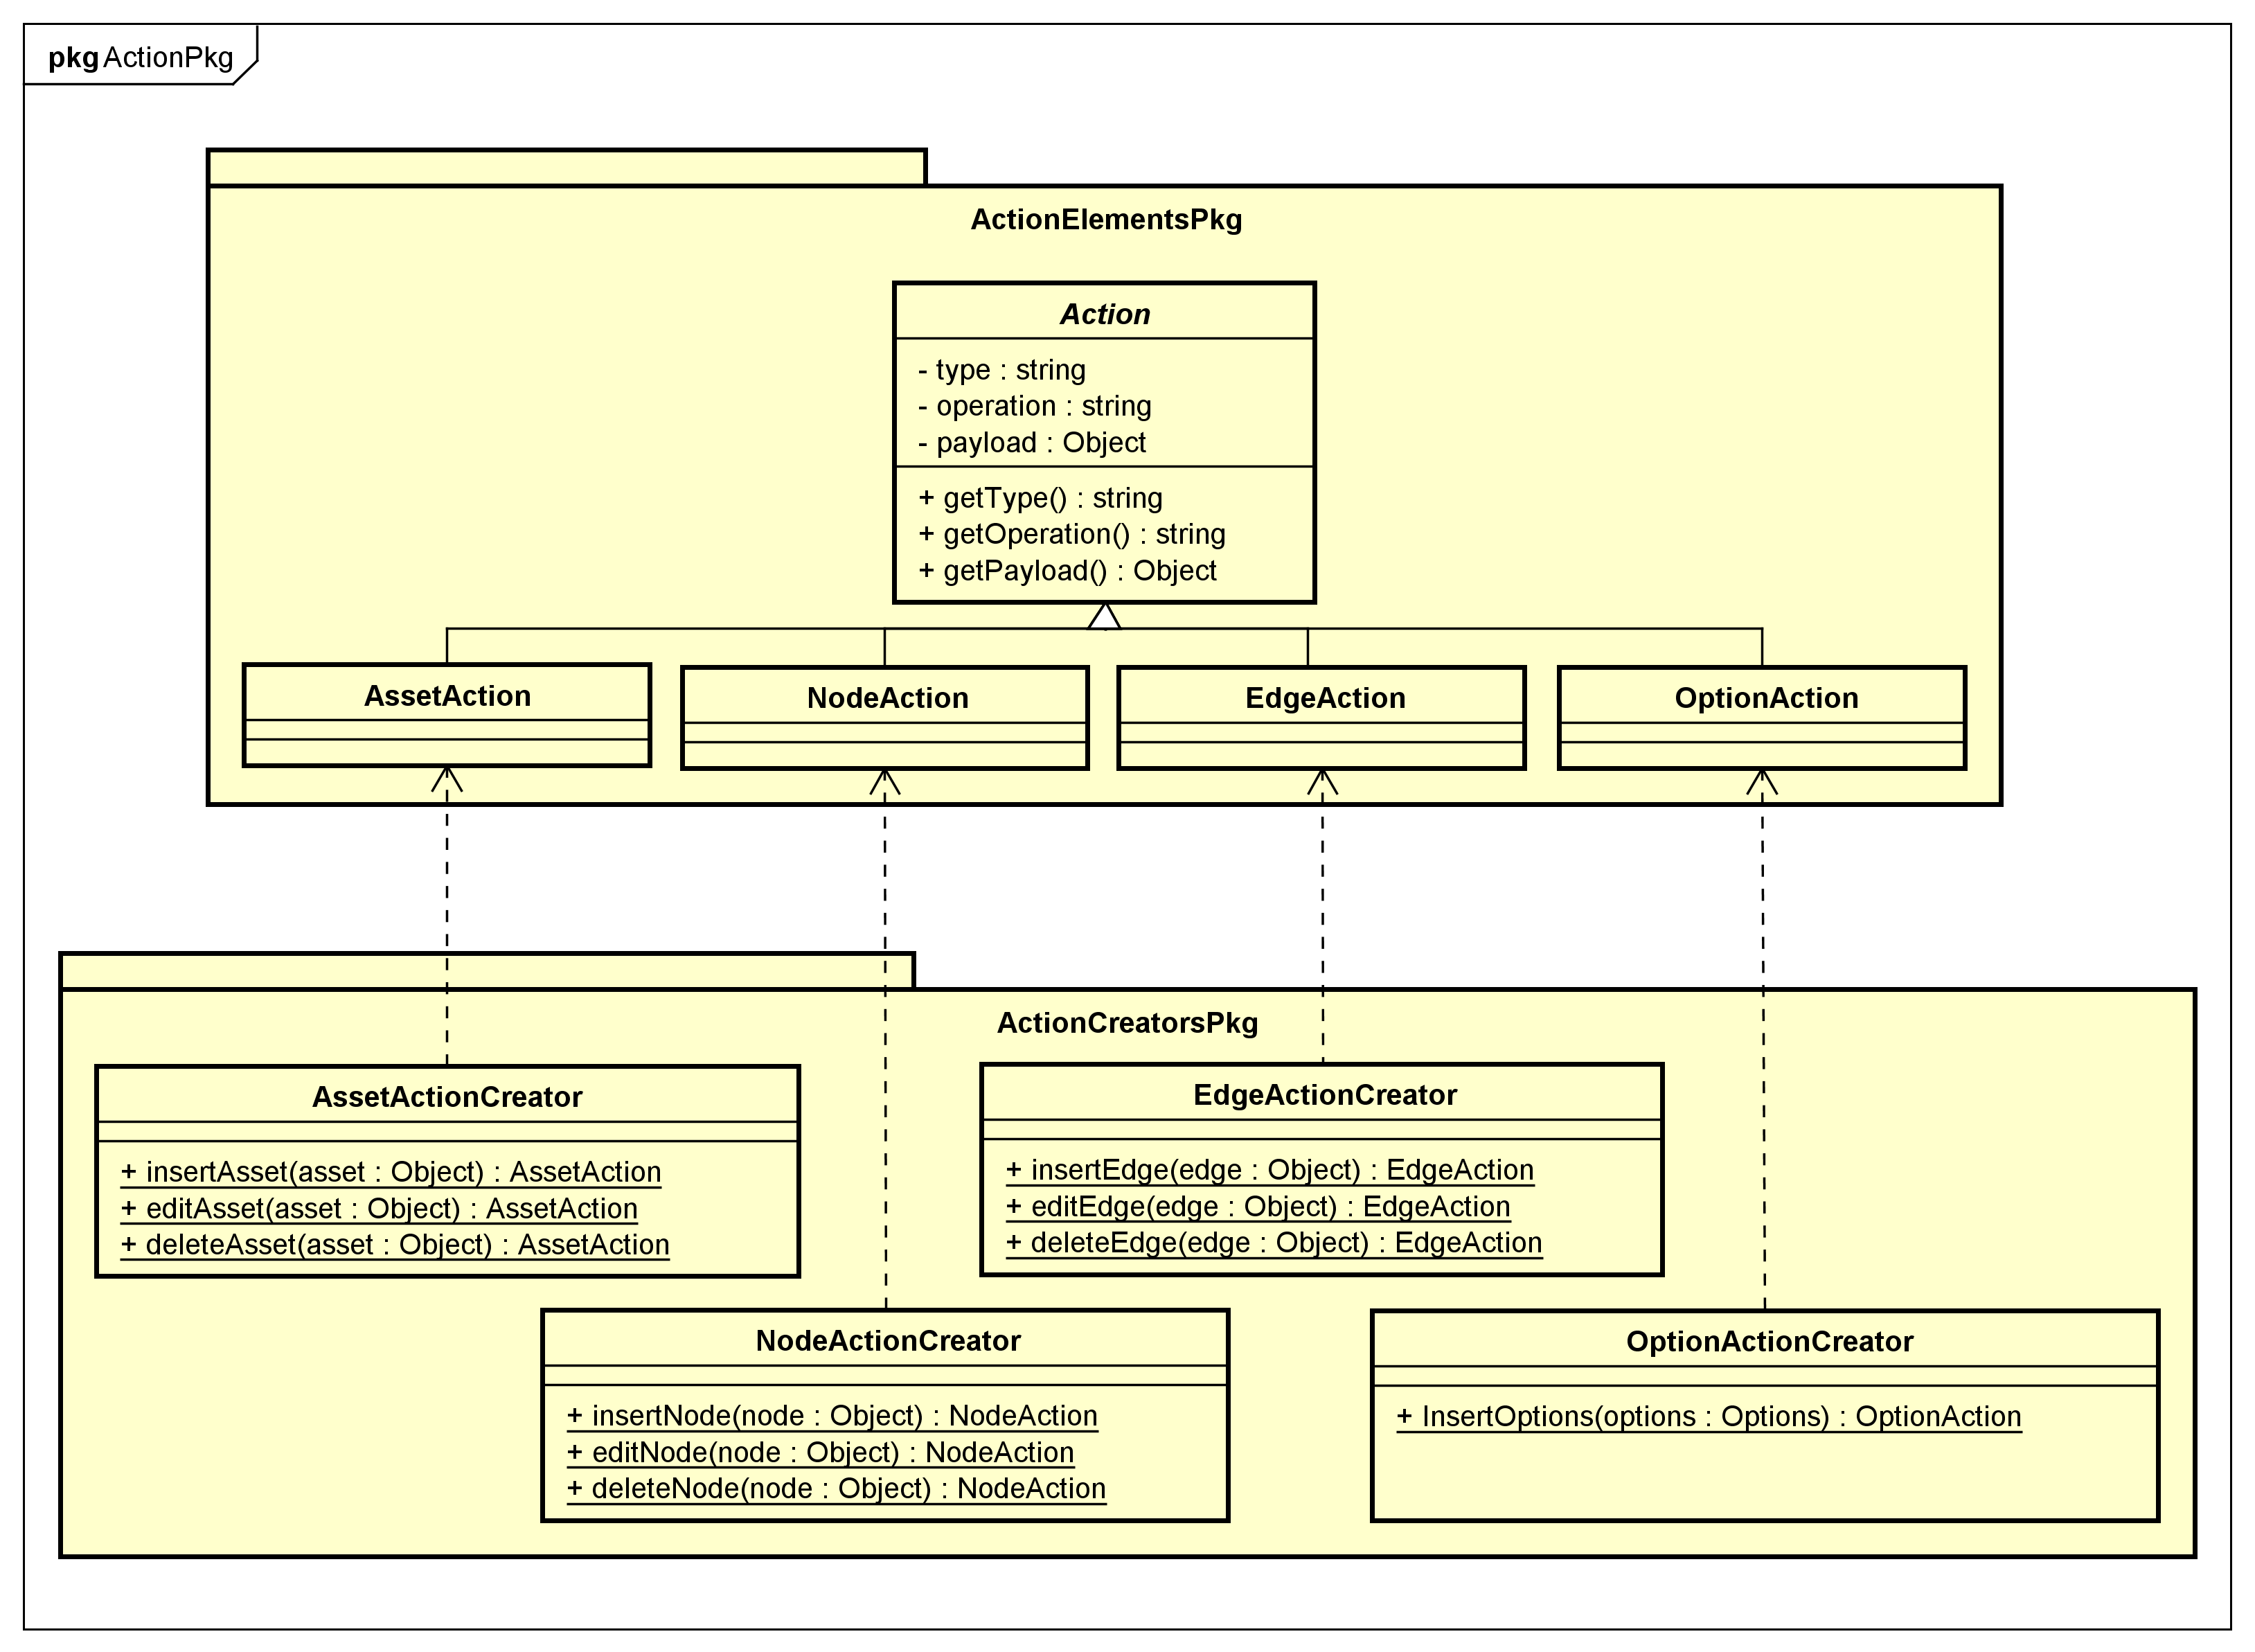
\includegraphics[width=\textwidth]{img/PkgDiagram/ActionPkg.png}
	\caption{Schema componente DeGeOP::ActionPkg}
\end{figure}
\subsubsection{Informazioni sul package}
\begin{itemize}
	\item \textbf{descrizione:} racchiude le componenti utilizzate per implementare le action dell'architettura Redux. Le action vengono create e ne viene fatto il dispatch verso lo store. Un reducer gestirà una action per produrre un cambiamento di stato sullo store;
	\item \textbf{padre:} \hyperref[pkg::DeGeOP]{DeGeOP};
	\item \textbf{package contenuti:}
	\begin{itemize}
		\item ActionPkg::\hyperref[pkg::ActionCreatorsPkg]{ActionCreatorsPkg};
		\item ActionPkg::\hyperref[pkg::ActionElementsPkg]{ActionElementsPkg}.
	\end{itemize}
	\item \textbf{interazioni con altri package:} 
	\begin{itemize}
		\item IN CallManagerPkg: dispatch di azioni;
		\item IN ReducerPkg: utilizzo di azioni ;
		\item IN ViewPkg: dispatch di azioni.
	\end{itemize}
	\item \textbf{classi contenute:}
	\begin{itemize}
		\item EdgeAction.
	\end{itemize}
\end{itemize}
\subsubsection{Classi}
\paragraph{EdgeAction}
\begin{itemize}
	\begin{figure}[H]
		\centering
		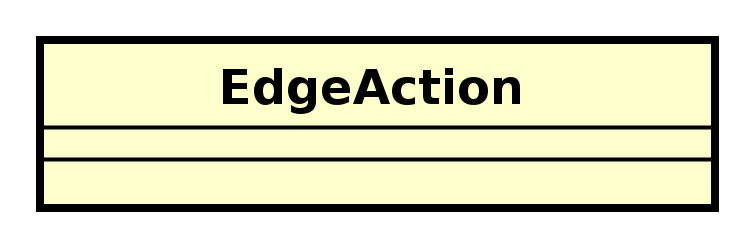
\includegraphics[width=0.3\textwidth]{./img/EdgeAction.png}
		\caption{Diagramma classe EdgeAction}
	\end{figure}
	\item \textbf{descrizione:} rappresenta un'azione relativa agli archi;
	\item \textbf{utilizzo:} l'azione viene creata da un apposito ActionCreator per essere poi inviata ad un reducer.
\end{itemize}
\newpage
\subsection{DeGeOP::ActionPkg::ActionElementsPkg}
\label{pkg::ActionElementsPkg}
\subsubsection{Informazioni sul package}
\begin{itemize}
	\item \textbf{descrizione:} racchiude le componenti che rappresentano effettivamente le azioni;
	\item \textbf{padre:} \hyperref[pkg::ActionPkg]{ActionPkg};
	\item \textbf{interazioni con altri package:} 
	\begin{itemize}
		\item IN ActionCreatorsPkg: creazione di azioni.
	\end{itemize}
	\item \textbf{classi contenute:}
	\begin{itemize}
		\item Action;
		\item AssetAction;
		\item NodeAction;
		\item OptionAction.
	\end{itemize}
\end{itemize}
\subsubsection{Classi}
\paragraph{Action}
\begin{itemize}
	\begin{figure}[H]
		\centering
		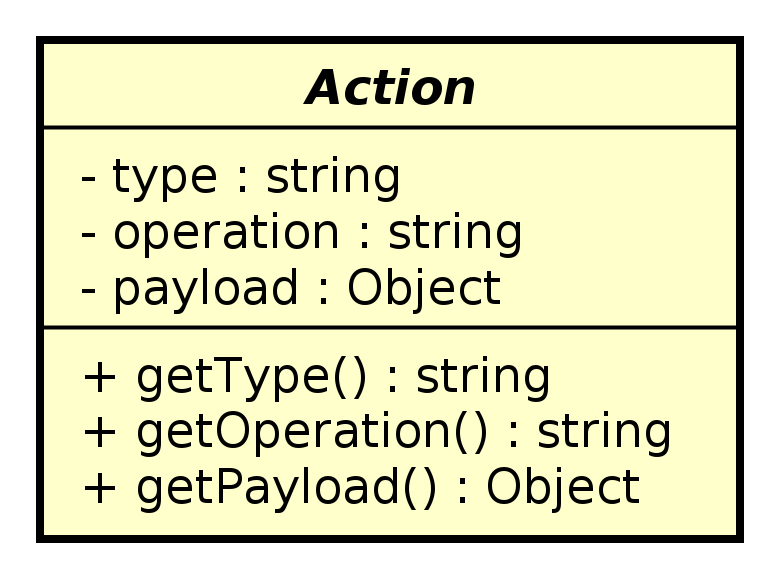
\includegraphics[width=0.3\textwidth]{./img/Action.png}
		\caption{Diagramma classe Action}
	\end{figure}
	\item \textbf{descrizione:} una classe astratta che rappresenta una generica azione di cui può essere fatto il dispatch;
	\item \textbf{utilizzo:} i suoi membri vengono usati dai reducer per completare una azione;
	\item \textbf{attributi:}
	\begin{itemize}
		\item -operation : string\begin{itemize}
			\item rappresenta l'operazione da eseguire.\end{itemize}
		\item -payload : Object\begin{itemize}
			\item rappresenta l'oggetto che descrive il cambiamento apportato dall'azione.\end{itemize}
		\item -type : string\begin{itemize}
			\item rappresenta la tipologia di elemento su cui eseguire l'azione.\end{itemize}
	\end{itemize}
	\item \textbf{metodi:}
	\begin{itemize}
		\item +getOperation() : string\newline
		il metodo ritorna l'operazione eseguita dall'azione
		\item +getPayload() : Object\newline
		il metodo ritorna il payload dell'oggetto
		\item +getType() : string\newline
		il metodo ritorna il tipo dell'azione
	\end{itemize}
\end{itemize}
\paragraph{AssetAction}
\begin{itemize}
	\begin{figure}[H]
		\centering
		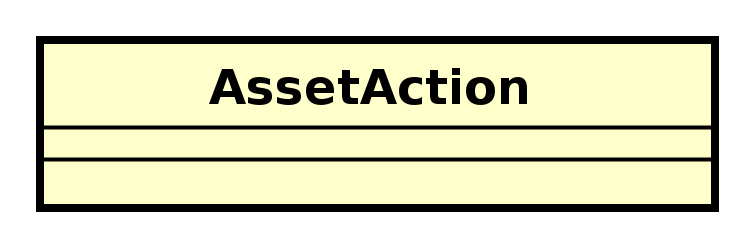
\includegraphics[width=0.3\textwidth]{./img/AssetAction.png}
		\caption{Diagramma classe AssetAction}
	\end{figure}
	\item \textbf{descrizione:} rappresenta un'azione relativa agli asset;
	\item \textbf{utilizzo:} l'azione viene creata da un apposito ActionCreator per essere poi inviata ad un reducer.
\end{itemize}
\paragraph{NodeAction}
\begin{itemize}
	\begin{figure}[H]
		\centering
		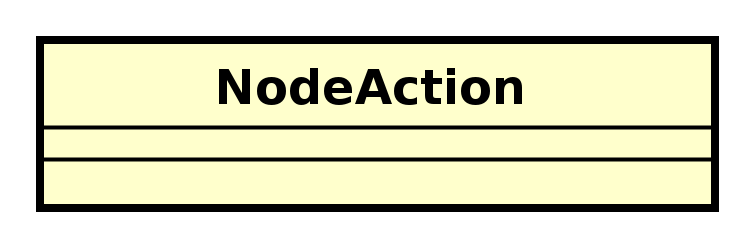
\includegraphics[width=0.3\textwidth]{./img/NodeAction.png}
		\caption{Diagramma classe NodeAction}
	\end{figure}
	\item \textbf{descrizione:} rappresenta un'azione relativa ai nodi;
	\item \textbf{utilizzo:} l'azione viene creata da un apposito ActionCreator per essere poi inviata ad un reducer.
\end{itemize}
\paragraph{OptionAction}
\begin{itemize}
	\begin{figure}[H]
		\centering
		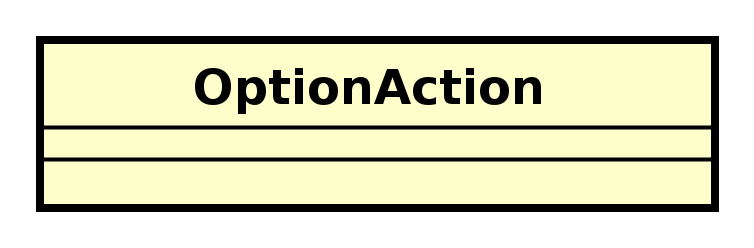
\includegraphics[width=0.3\textwidth]{./img/OptionAction.png}
		\caption{Diagramma classe OptionAction}
	\end{figure}
	\item \textbf{descrizione:} rappresenta un'azione relativa all'oggetto option;
	\item \textbf{utilizzo:} l'azione viene creata da un apposito ActionCreator per essere poi inviata ad un reducer;
	\item \textbf{relazioni con altre classi:} 
	\begin{itemize}
		\item IN OptionActionCreator.
	\end{itemize}
\end{itemize}
\newpage
\subsection{DeGeOP::ActionPkg::ActionCreatorsPkg}
\label{pkg::ActionCreatorsPkg}
\subsubsection{Informazioni sul package}
\begin{itemize}
	\item \textbf{descrizione:} racchiude le componenti che gestiscono la creazione delle azioni;
	\item \textbf{padre:} \hyperref[pkg::ActionPkg]{ActionPkg};
	\item \textbf{interazioni con altri package:} 
	\begin{itemize}
		\item OUT ActionElementsPkg: creazione di azioni.
	\end{itemize}
	\item \textbf{classi contenute:}
	\begin{itemize}
		\item AssetActionCreator;
		\item EdgeActionCreator;
		\item NodeActionCreator;
		\item OptionActionCreator.
	\end{itemize}
\end{itemize}
\subsubsection{Classi}
\paragraph{AssetActionCreator}
\begin{itemize}
	\begin{figure}[H]
		\centering
		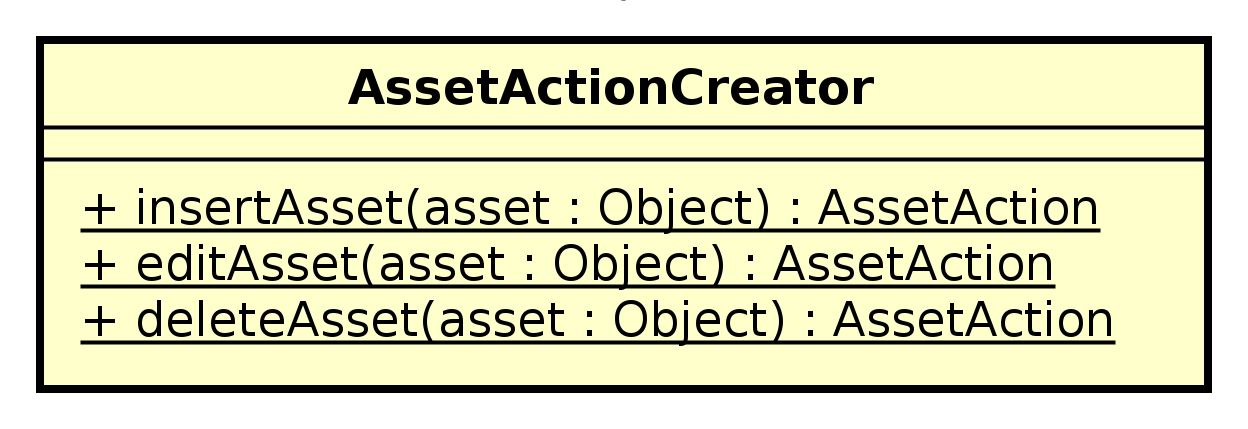
\includegraphics[width=0.3\textwidth]{./img/AssetActionCreator.png}
		\caption{Diagramma classe AssetActionCreator}
	\end{figure}
	\item \textbf{descrizione:} rappresenta la factory di azioni relative agli asset;
	\item \textbf{utilizzo:} i suoi metodi sono chiamati dalla View e dal CallManager per la creazione di azioni relative agli asset;
	\item \textbf{metodi:}
	\begin{itemize}
		\item +deleteAsset(asset) : AssetAction\newline
		il metodo crea l'azione relativa all'eliminazione dell'asset ricevuto in input
		\begin{itemize}
			\item asset : Object\\
			oggetto contenente i parametri di un Asset che dovrà essere eliminato.
		\end{itemize}
		\item +editAsset(asset) : AssetAction\newline
		il metodo crea l'azione relativa alla modifica di un asset
		\begin{itemize}
			\item asset : Object\\
			oggetto contenente i parametri di un Asset che dovrà essere modificato nello store.
		\end{itemize}
		\item +insertAsset(asset) : AssetAction\newline
		il metodo crea l'azione relativa all'inserimento di un nuovo asset
		\begin{itemize}
			\item asset : Object\\
			oggetto contenente i parametri di un Asset che dovrà essere inserito nello store.
		\end{itemize}
	\end{itemize}
\end{itemize}
\paragraph{EdgeActionCreator}
\begin{itemize}
	\begin{figure}[H]
		\centering
		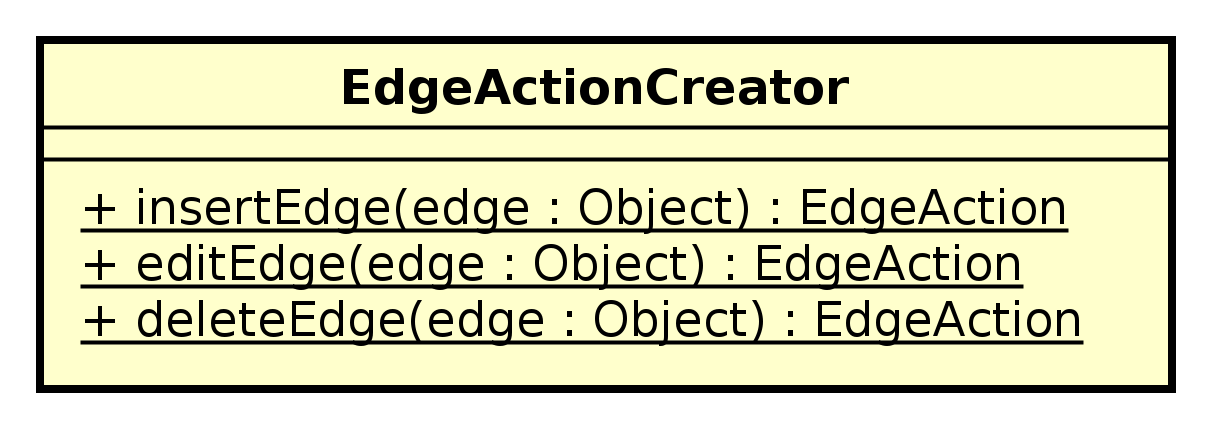
\includegraphics[width=0.3\textwidth]{./img/EdgeActionCreator.png}
		\caption{Diagramma classe EdgeActionCreator}
	\end{figure}
	\item \textbf{descrizione:} rappresenta la factory di azioni relative agli archi;
	\item \textbf{utilizzo:} i suoi metodi sono chiamati dalla View e dal CallManager per la creazione di azioni relative agli archi;
	\item \textbf{metodi:}
	\begin{itemize}
		\item +deleteEdge(edge) : EdgeAction\newline
		il metodo crea l'azione relativa all'eliminazione di un arco
		\begin{itemize}
			\item edge : Object\\
			oggetto contenente i parametri di un arco che dovrà essere eliminato.
		\end{itemize}
		\item +editEdge(edge) : EdgeAction\newline
		il metodo crea l'azione relativa alla modifica di un arco
		\begin{itemize}
			\item edge : Object\\
			oggetto contenente i parametri di un arco che dovrà essere modificato nello store.
		\end{itemize}
		\item +insertEdge(edge) : EdgeAction\newline
		il metodo crea l'azione relativa all'inserimento di un nuovo arco
		\begin{itemize}
			\item edge : Object\\
			oggetto contenente i parametri di un arco che dovrà essere inserito nello store.
		\end{itemize}
	\end{itemize}
\end{itemize}
\paragraph{NodeActionCreator}
\begin{itemize}
	\begin{figure}[H]
		\centering
		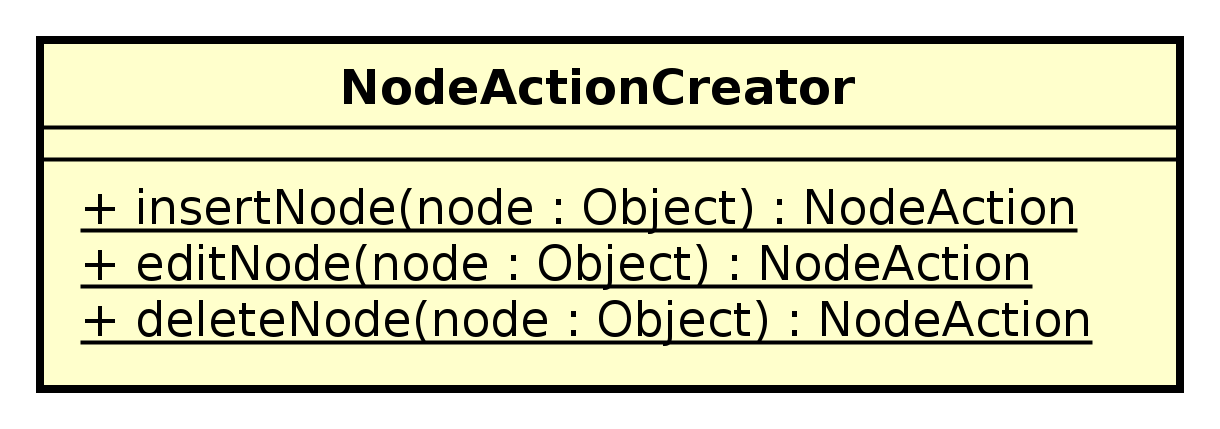
\includegraphics[width=0.3\textwidth]{./img/NodeActionCreator.png}
		\caption{Diagramma classe NodeActionCreator}
	\end{figure}
	\item \textbf{descrizione:} rappresenta la factory di azioni relative ai nodi;
	\item \textbf{utilizzo:} i suoi metodi sono chiamati dalla View e dal CallManager per la creazione di azioni relative ai nodi;
	\item \textbf{metodi:}
	\begin{itemize}
		\item +deleteNode(node) : NodeAction\newline
		il metodo crea l'azione relativa all'eliminazione di un nodo
		\begin{itemize}
			\item node : Object\\
			oggetto contenente i parametri di un nodo che dovrà essere eliminato.
		\end{itemize}
		\item +editNode(node) : NodeAction\newline
		il metodo crea l'azione relativa alla modifica di un nodo
		\begin{itemize}
			\item node : Object\\
			oggetto contenente i parametri di un nodo che dovrà essere modificato nello store.
		\end{itemize}
		\item +insertNode(node) : NodeAction\newline
		il metodo crea l'azione relativa all'inserimento di un nuovo nodo
		\begin{itemize}
			\item node : Object\\
			oggetto contenente i parametri di un nodo che dovrà essere inserito nello store.
		\end{itemize}
	\end{itemize}
\end{itemize}
\paragraph{OptionActionCreator}
\begin{itemize}
	\begin{figure}[H]
		\centering
		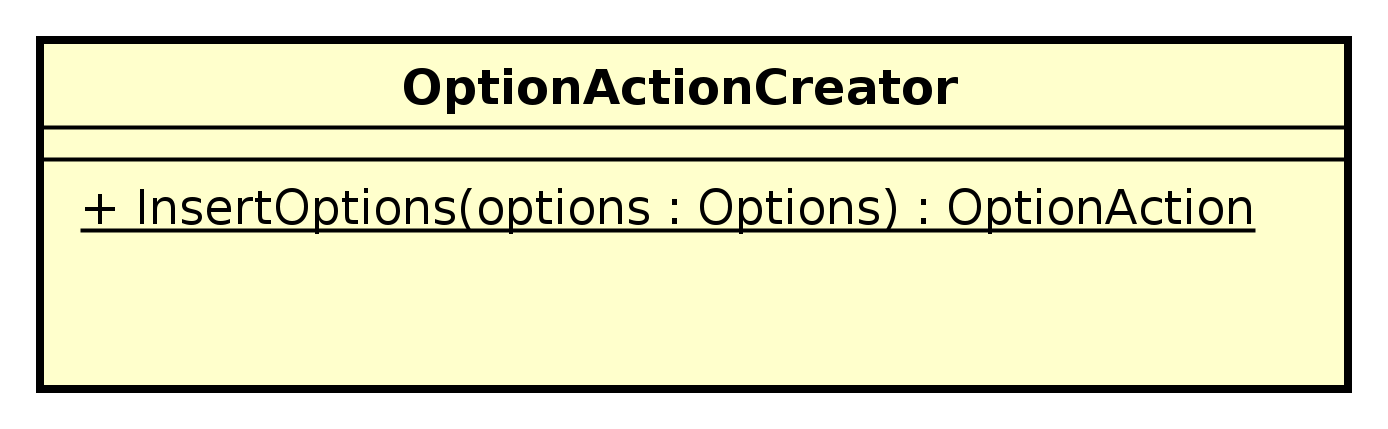
\includegraphics[width=0.3\textwidth]{./img/OptionActionCreator.png}
		\caption{Diagramma classe OptionActionCreator}
	\end{figure}
	\item \textbf{descrizione:} rappresenta la factory di azioni relative agli asset;
	\item \textbf{utilizzo:} i suoi metodi sono chiamati dalla View e dal CallManager per la creazione di azioni relative agli asset;
	\item \textbf{metodi:}
	\begin{itemize}
		\item +insertOptions() : OptionAction\newline
		il metodo crea l'azione relativa all'inserimento dell'oggetto options dello store
	\end{itemize}
	\item \textbf{relazioni con altre classi:} 
	\begin{itemize}
		\item OUT OptionAction.
	\end{itemize}
\end{itemize}
\newpage
\subsection{DeGeOP::ViewPkg}
\label{pkg::ViewPkg}
\begin{figure}[H]
	\centering
	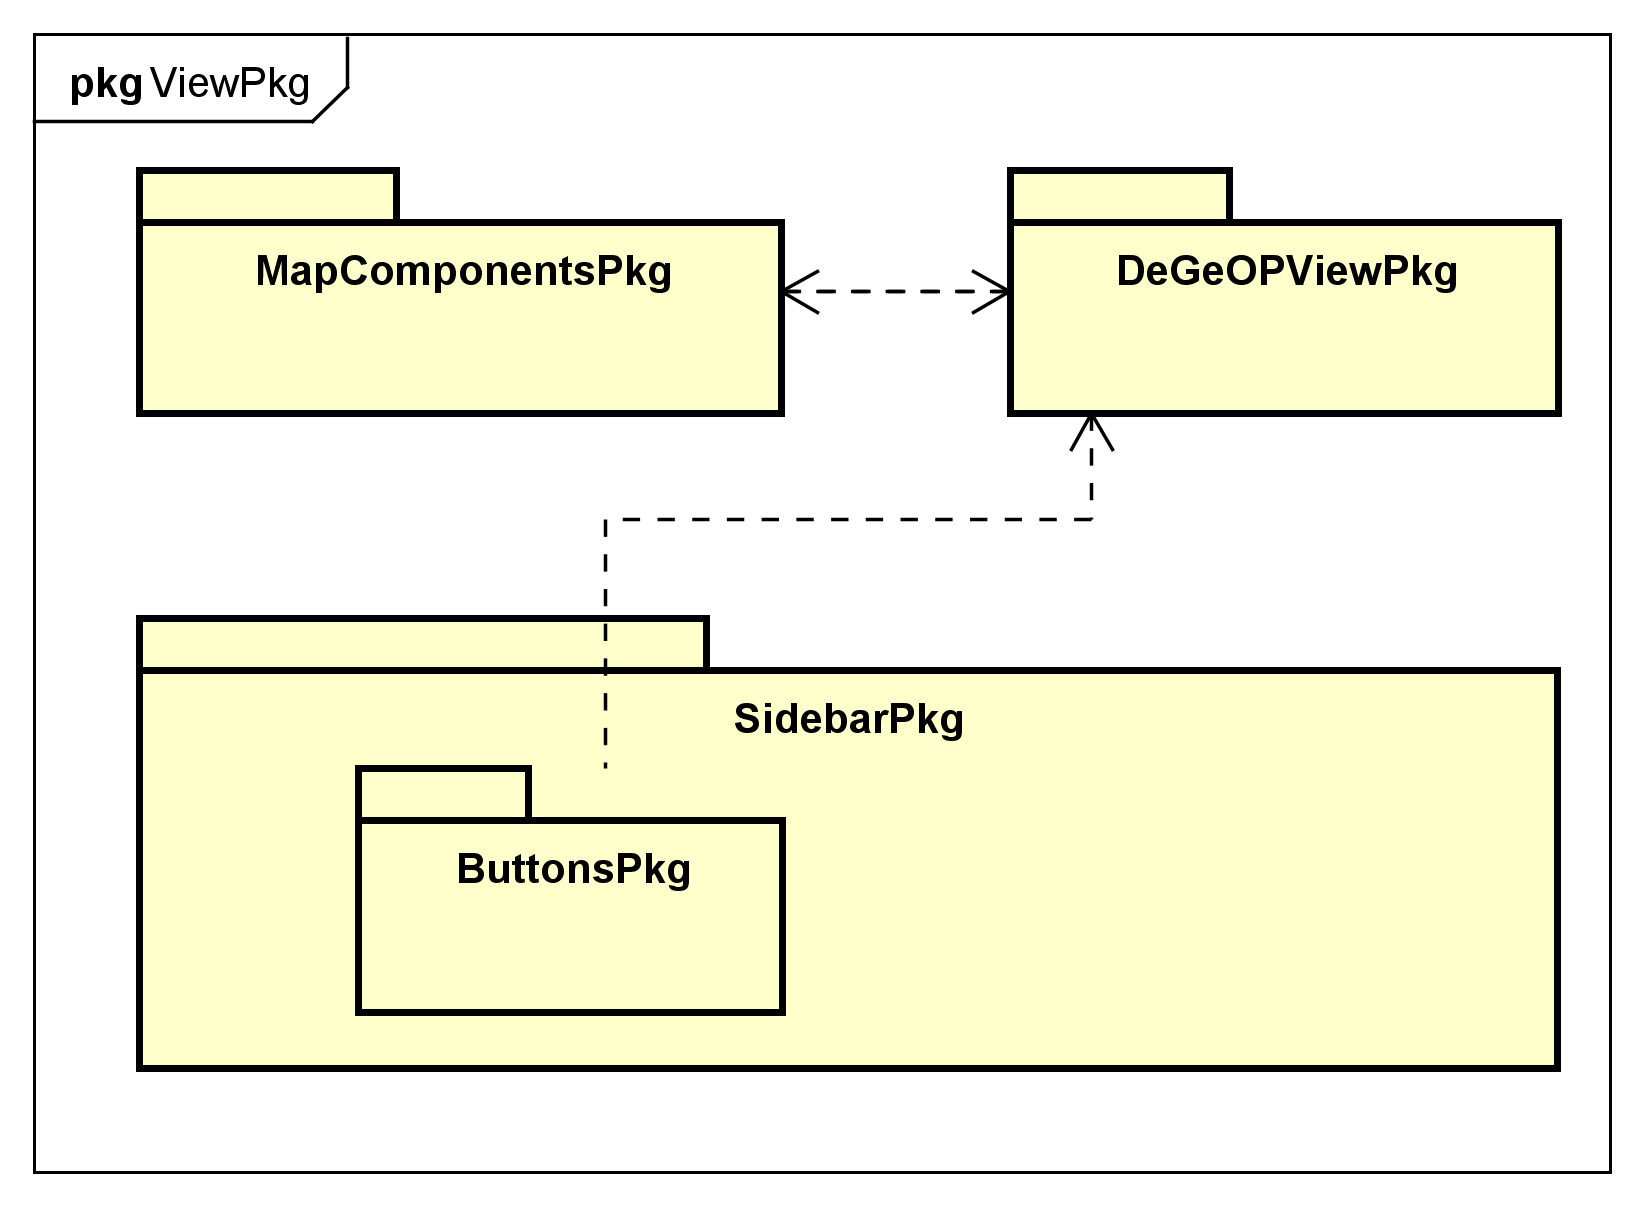
\includegraphics[width=\textwidth]{img/PkgDiagram/ViewPkg.png}
	\caption{Schema componente DeGeOP::ViewPkg}
\end{figure}
\subsubsection{Informazioni sul package}
\begin{itemize}
	\item \textbf{descrizione:} racchiude le componenti per la visualizzazione dell'interfaccia utente;
	\item \textbf{padre:} \hyperref[pkg::DeGeOP]{DeGeOP};
	\item \textbf{package contenuti:}
	\begin{itemize}
		\item ViewPkg::\hyperref[pkg::DeGeOPViewPkg]{DeGeOPViewPkg};
		\item ViewPkg::\hyperref[pkg::MapComponentsPkg]{MapComponentsPkg};
		\item ViewPkg::\hyperref[pkg::SidebarPkg]{SidebarPkg}.
	\end{itemize}
	\item \textbf{interazioni con altri package:} 
	\begin{itemize}
		\item OUT ActionPkg: dispatch di azioni;
		\item OUT Alexa voice service: gestore vocale;
		\item OUT Hammer: gestione gesture ;
		\item OUT Openlayers: gestione mappa;
		\item OUT React: utilizzo componenti react;
		\item OUT ReactToolbox: utilizzo componenti material design;
		\item OUT Redux: utilizzo metodo dispatch;
		\item OUT StorePkg: subscribe sullo store.
	\end{itemize}
\end{itemize}
\newpage
\subsection{DeGeOP::ViewPkg::DeGeOPViewPkg}
\label{pkg::DeGeOPViewPkg}
\begin{figure}[H]
	\centering
	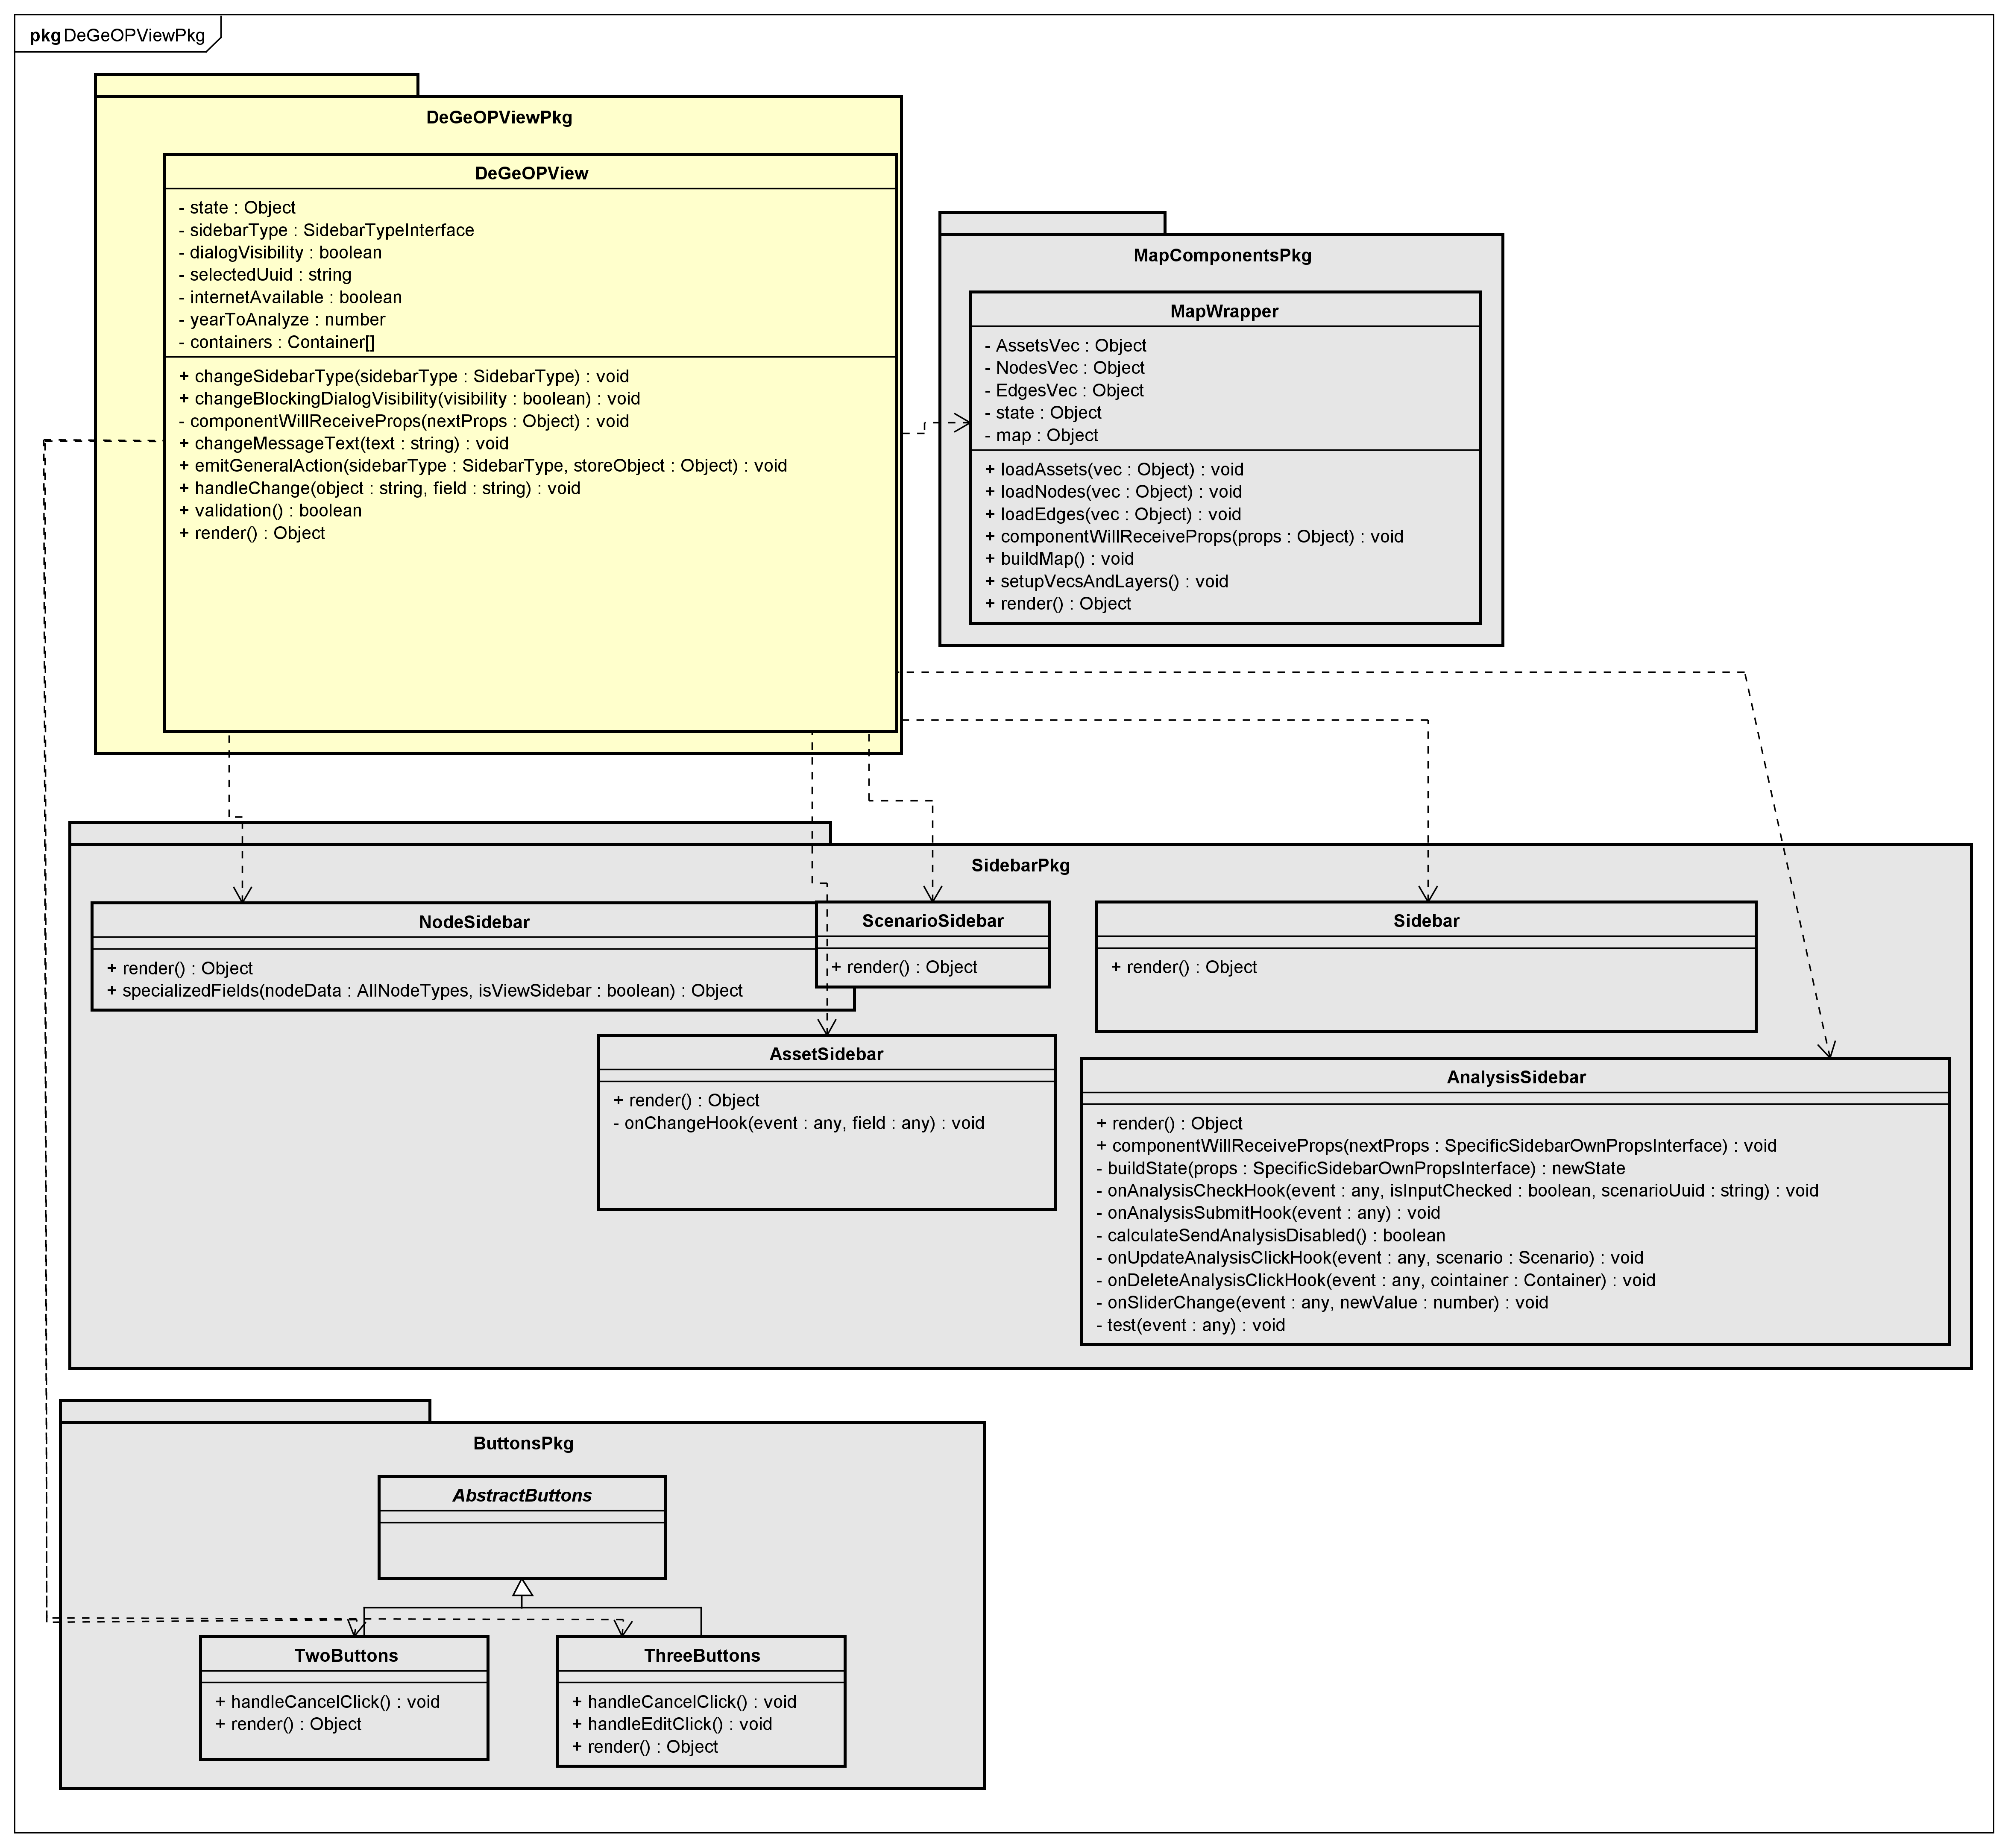
\includegraphics[width=\textwidth]{img/PkgDiagram/DeGeOPViewPkg.png}
	\caption{Schema componente DeGeOP::ViewPkg::DeGeOPViewPkg}
\end{figure}
\subsubsection{Informazioni sul package}
\begin{itemize}
	\item \textbf{descrizione:} racchiude la componente principale della view;
	\item \textbf{padre:} \hyperref[pkg::ViewPkg]{ViewPkg};
	\item \textbf{interazioni con altri package:} 
	\begin{itemize}
		\item IN MapComponentsPkg: utilizzo di componenti grafiche;
		\item OUT MapComponentsPkg: utilizzo di componenti grafiche;
		\item OUT SidebarPkg: utilizzo della sidebar.
	\end{itemize}
	\item \textbf{classi contenute:}
	\begin{itemize}
		\item DeGeOPView.
	\end{itemize}
\end{itemize}
\subsubsection{Classi}
\paragraph{DeGeOPView}
\begin{itemize}
	\begin{figure}[H]
		\centering
		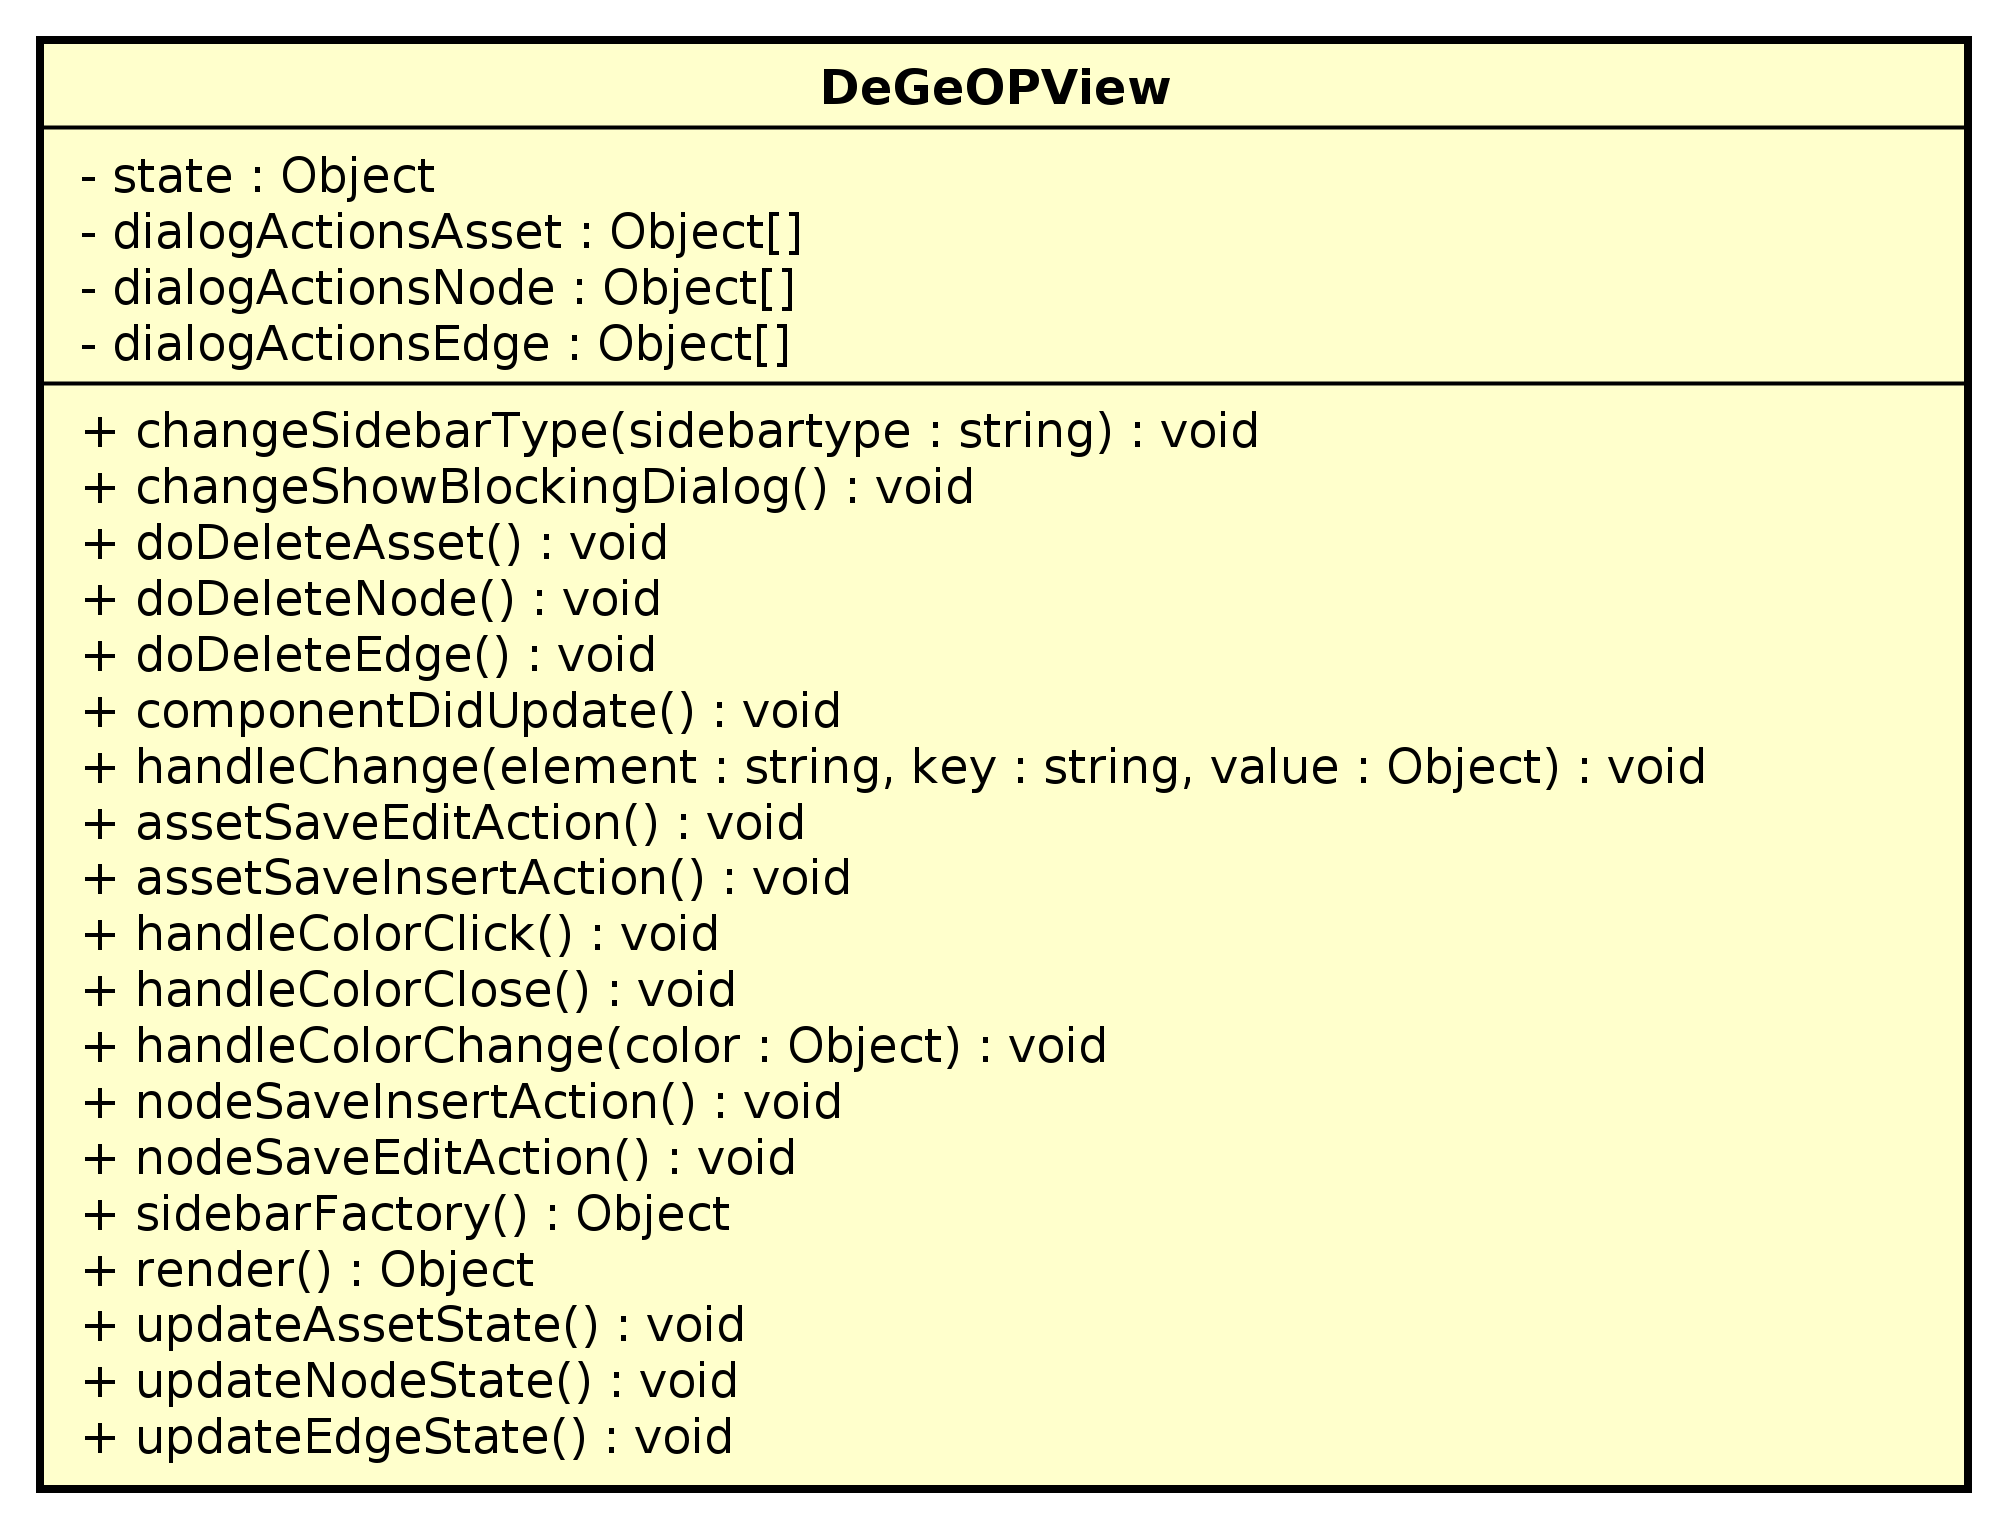
\includegraphics[width=0.3\textwidth]{./img/DeGeOPView.png}
		\caption{Diagramma classe DeGeOPView}
	\end{figure}
	\item \textbf{descrizione:} rappresenta l'oggetto grafico radice, che comprende l'intera View del prodotto;
	\item \textbf{utilizzo:} i suoi metodi setter sono richiamati da ConcreteDeGeOPViewBuilder per impostare i suoi campi dati. La classe effettua il subscribe sullo Store per ricevere gli aggiornamenti ;
	\item \textbf{attributi:}
	\begin{itemize}
		\item -containers : Container\begin{itemize}
			\item La lista di container delle analisi.\end{itemize}
		\item -dialogVisibility : boolean\begin{itemize}
			\item La visibilità del dialog.\end{itemize}
		\item -internetAvailable : boolean\begin{itemize}
			\item Se internet è disponibile o meno.\end{itemize}
		\item -selectedUuid : string\begin{itemize}
			\item L'uuid selezionato dell'elemento selezionato al momento.\end{itemize}
		\item -sidebarType : SidebarTypeInterface\begin{itemize}
			\item Il tipo di sidebar visualizzata.\end{itemize}
		\item -state : Object\begin{itemize}
			\item rappresenta lo stato di DeGeOPView, ovvero i dati temporanei che l'utente inserisce prima che vengano inseriti nello store.\end{itemize}
		\item -yearToAnalyze : number\begin{itemize}
			\item L'anno da prendere in esame per l'analisi di danno.\end{itemize}
	\end{itemize}
	\item \textbf{metodi:}
	\begin{itemize}
		\item +changeBlockingDialogVisibility() : void\newline
		Cambia la visibilità del blocking dialog
		\item +changeMessageText(text) : void\newline
		cambia il testo del MessageWrapper visualizzato
		\begin{itemize}
			\item text : string\\
			Il testo del messaggio.
		\end{itemize}
		\item +changeSidebarType(sidebarType) : void\newline
		Cambia il tipo di sidebar
		\begin{itemize}
			\item sidebarType : Object\\
			Il tipo di Sidebar.
		\end{itemize}
		\item +componentWillReceiveProps(nextProps) : void\newline
		Gestisce i cambiamenti di state in base alle nuove props
		\begin{itemize}
			\item nextProps : Object\\
			Le nuove props che la componente riceve.
		\end{itemize}
		\item +emitGeneralAction() : void\newline
		Emette le azioni verso lo store in base al SidebarType
		\item +handleChange(element, key, value) : void\newline
		il metodo gestisce il cambiamento di stato di DeGeOPView relativamente ai campi dati compilati dall'utente
		\begin{itemize}
			\item element : string\\
			indica il campo dati dello stato di DeGeOPView da cambiare. Può assumere i valori:
			asset, node, edge, common.
			\item key : string\\
			indica il campo dati dell'oggetto descritto da element che dovrà essere modificato.
			\item value : Object\\
			indica il valore da inserire nell'oggetto descritto da element, nel campo dati descritto da key.
		\end{itemize}
		\item +render() : Object\newline
		il metodo gestisce il render di DeGeOPView, composta da una sidebar e da un MapWrapper
		\item +validation() : void\newline
		Valida i dati inseriti dall'utente, cambiando lo state con i risultati della validazione
	\end{itemize}
\end{itemize}
\newpage
\subsection{DeGeOP::ViewPkg::MapComponentsPkg}
\label{pkg::MapComponentsPkg}
\begin{figure}[H]
	\centering
	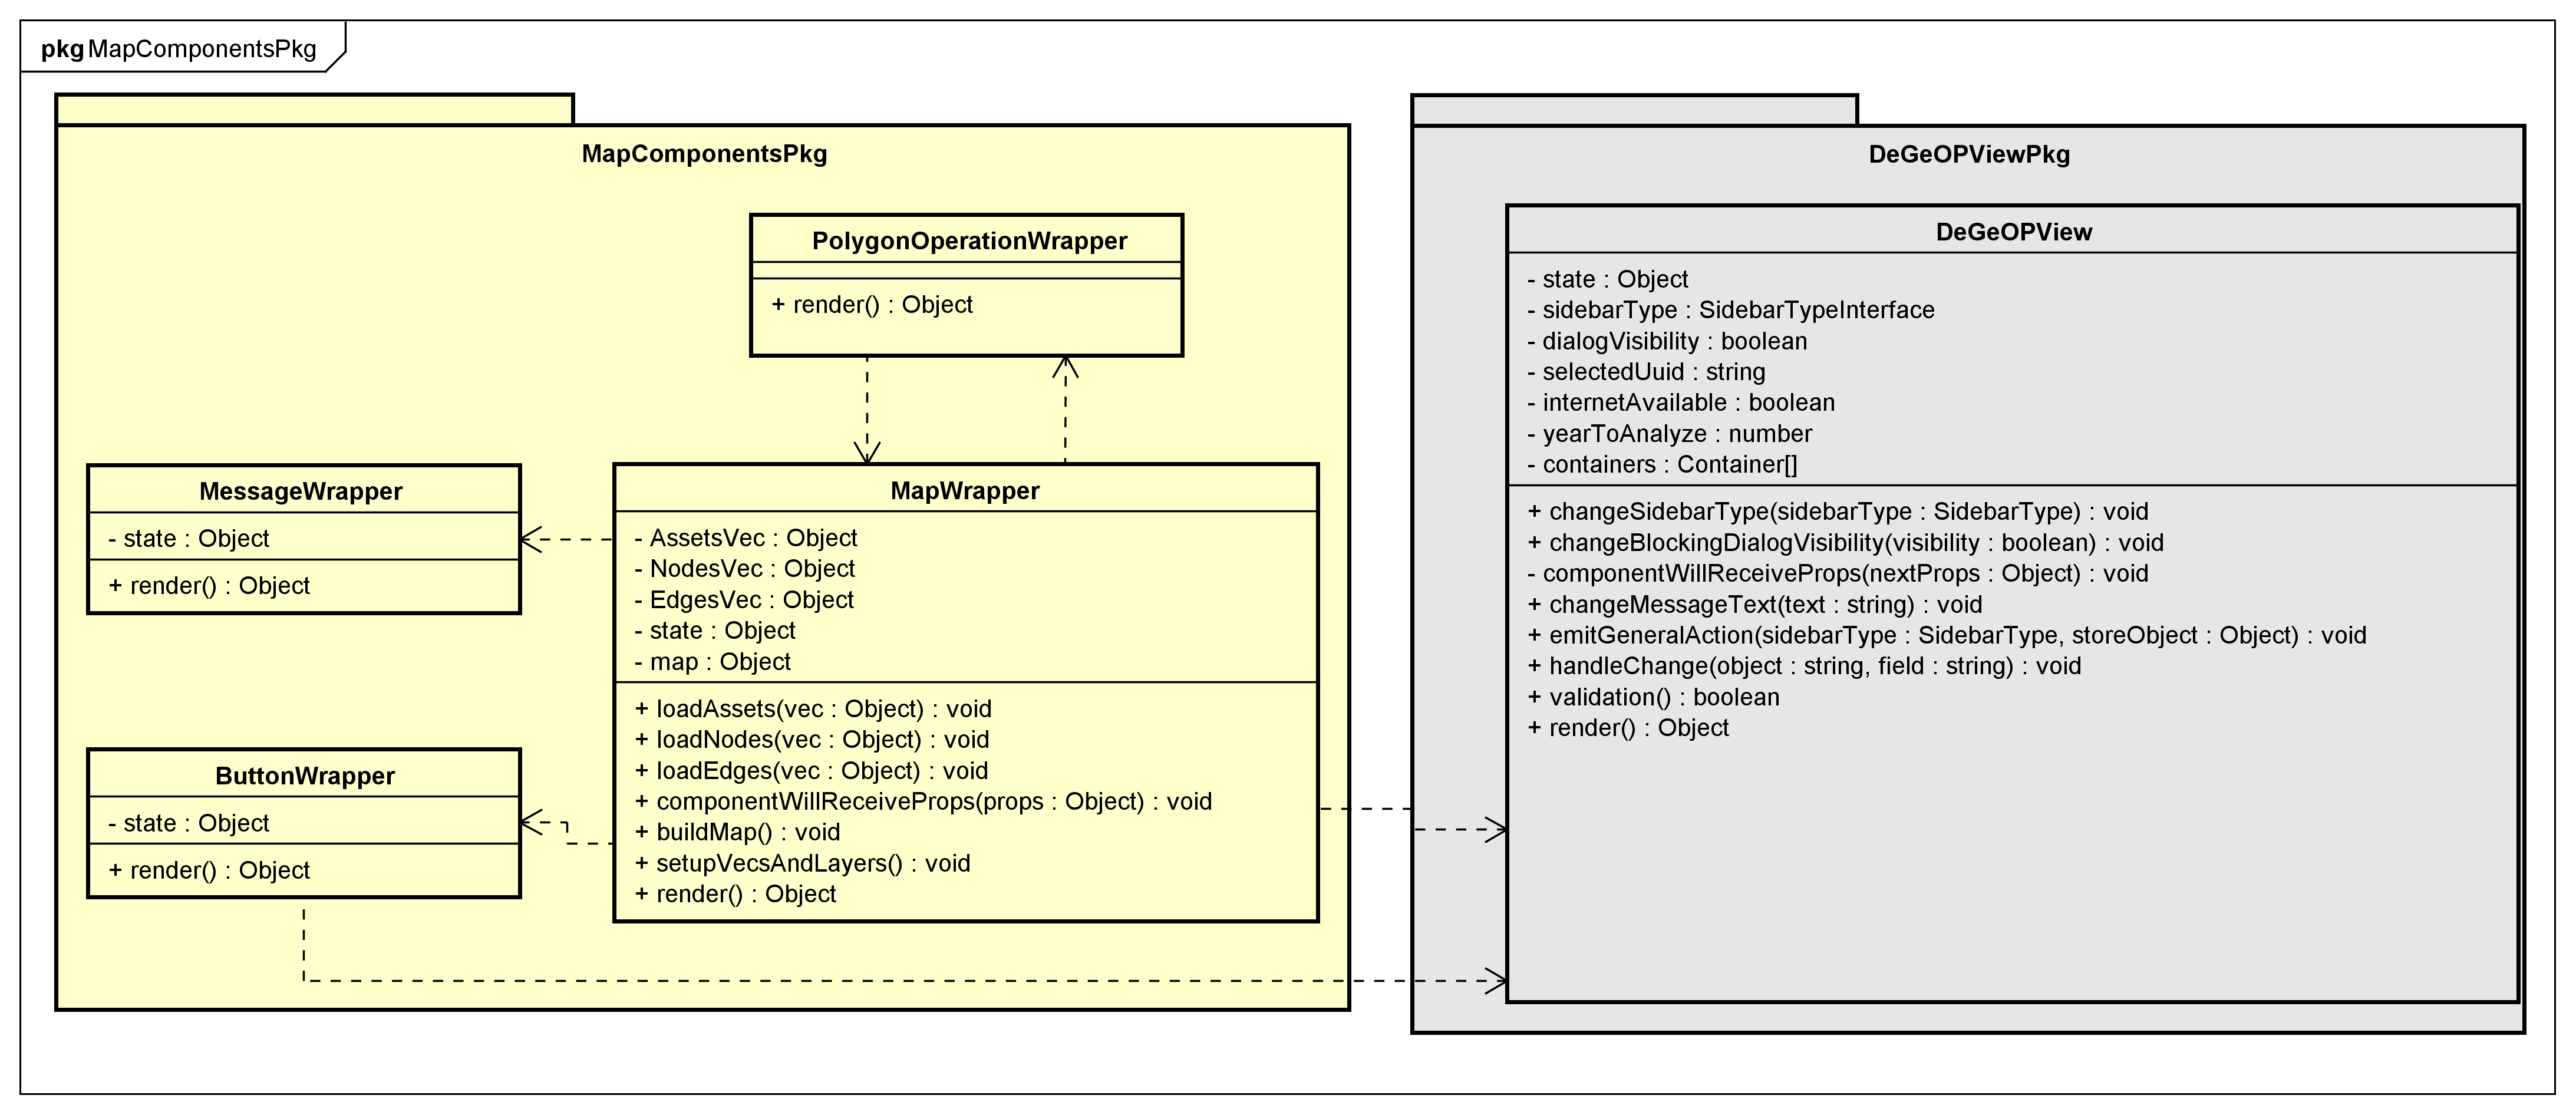
\includegraphics[width=\textwidth]{img/PkgDiagram/MapComponentsPkg.png}
	\caption{Schema componente DeGeOP::ViewPkg::MapComponentsPkg}
\end{figure}
\subsubsection{Informazioni sul package}
\begin{itemize}
	\item \textbf{descrizione:} racchiude le componenti relative alla mappa e ai pulsanti sopra di essa;
	\item \textbf{padre:} \hyperref[pkg::ViewPkg]{ViewPkg};
	\item \textbf{interazioni con altri package:} 
	\begin{itemize}
		\item IN DeGeOPViewPkg: utilizzo di componenti grafiche;
		\item OUT DeGeOPViewPkg: utilizzo di componenti grafiche;
		\item OUT Openlayers: gestione mappa.
	\end{itemize}
	\item \textbf{classi contenute:}
	\begin{itemize}
		\item ButtonWrapper;
		\item MapWrapper;
		\item MessageWrapper;
		\item PolygonOperationWrapper.
	\end{itemize}
\end{itemize}
\subsubsection{Classi}
\paragraph{ButtonWrapper}
\begin{itemize}
	\begin{figure}[H]
		\centering
		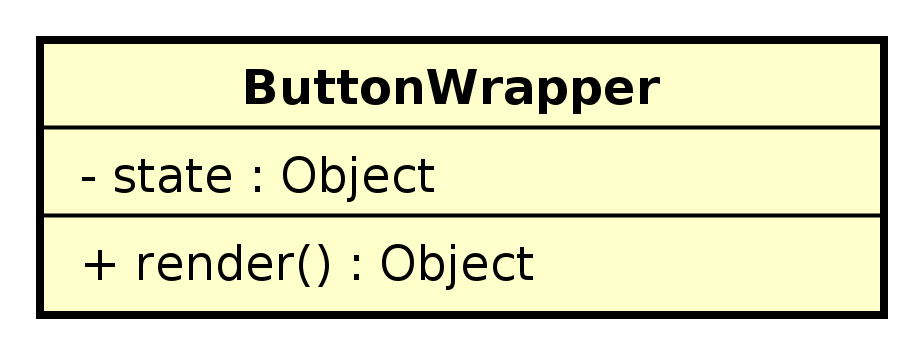
\includegraphics[width=0.3\textwidth]{./img/ButtonWrapper.png}
		\caption{Diagramma classe ButtonWrapper}
	\end{figure}
	\item \textbf{descrizione:} rappresenta una classe wrapper per visualizzare una serie di bottoni con cui è possibile eseguire varie operazioni;
	\item \textbf{utilizzo:} viene utilizzato per mostrare sulla mappa una serie di bottoni;
	\item \textbf{attributi:}
	\begin{itemize}
		\item -state : Object\begin{itemize}
			\item rappresenta lo stato del ButtonWrapper.\end{itemize}
	\end{itemize}
	\item \textbf{relazioni con altre classi:} 
	\begin{itemize}
		\item IN MapWrapper.
	\end{itemize}
\end{itemize}
\paragraph{MapWrapper}
\begin{itemize}
	\begin{figure}[H]
		\centering
		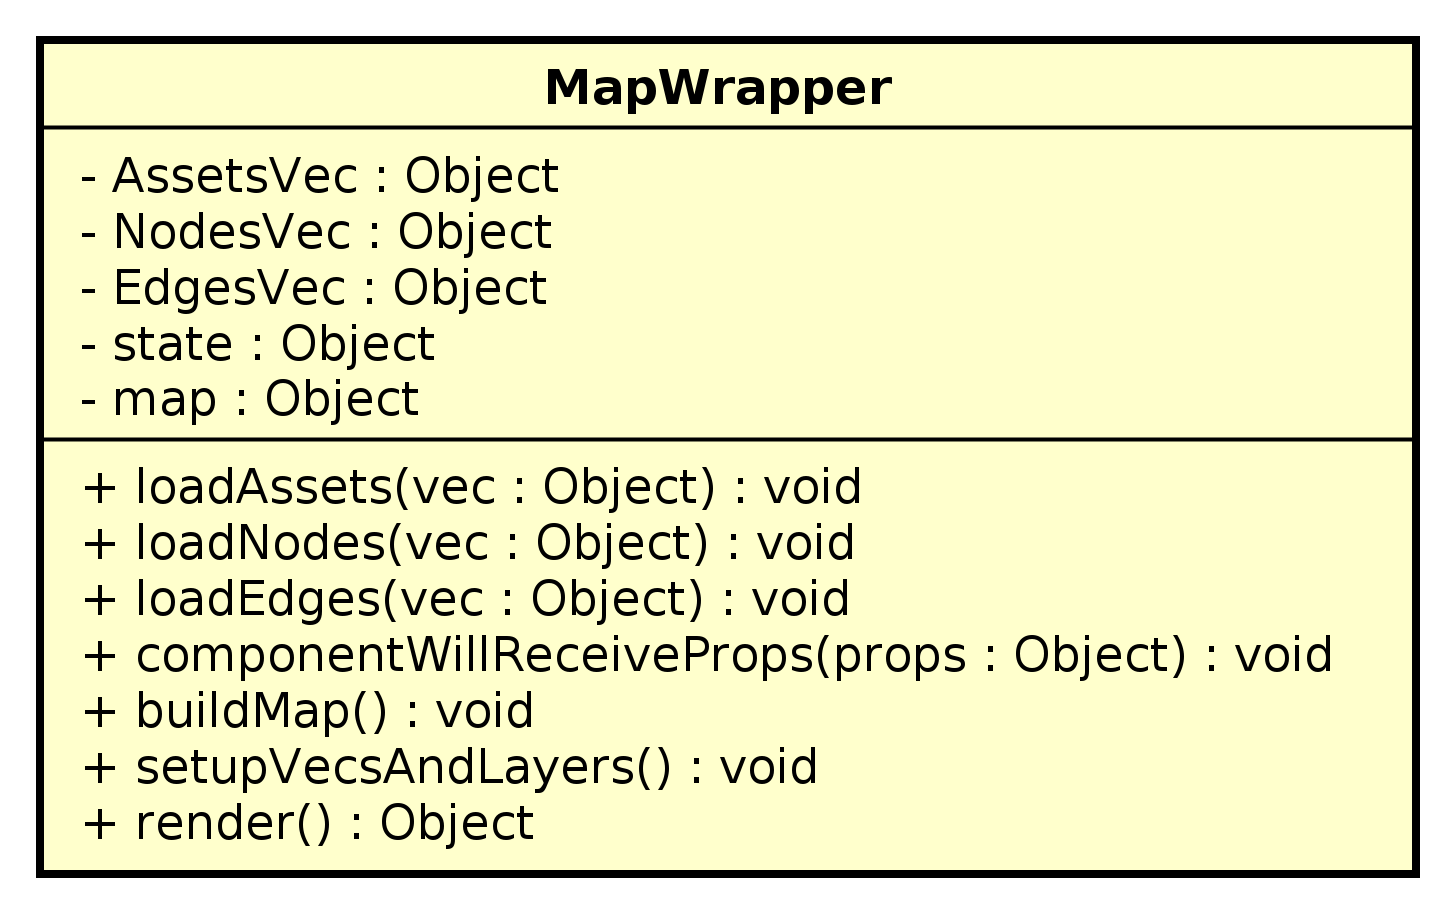
\includegraphics[width=0.3\textwidth]{./img/MapWrapper.png}
		\caption{Diagramma classe MapWrapper}
	\end{figure}
	\item \textbf{descrizione:} rappresenta una classe wrapper per visualizzare la mappa;
	\item \textbf{utilizzo:} viene utilizzata per visualizzare una mappa e permettere all'utente di interagire con essa;
	\item \textbf{attributi:}
	\begin{itemize}
		\item -assetsVec : Object\begin{itemize}
			\item contiene gli oggetti geometrici relativi agli asset da disegnare sulla mappa.\end{itemize}
		\item -edgesVec : Object\begin{itemize}
			\item contiene gli oggetti geometrici relativi agli asset da disegnare sulla mappa.\end{itemize}
		\item -map : Object\begin{itemize}
			\item oggetto che contiene lo stato della mappa.\end{itemize}
		\item -nodesVec : Object\begin{itemize}
			\item contiene gli oggetti geometrici relativi ai nodi da disegnare sulla mappa.\end{itemize}
		\item -state : Object\begin{itemize}
			\item contiene lo stato della classe MapWrapper.\end{itemize}
	\end{itemize}
	\item \textbf{metodi:}
	\begin{itemize}
		\item +buildMap() : void\newline
		il metodo costruisce la mappa
		\item +componentWillReceiveProps(props) : void\newline
		il metodo viene richiamato quando la componente MapWrapper sta per ricevere nuovi props
		\begin{itemize}
			\item props : Object\\
			props da ricevere.
		\end{itemize}
		\item +loadAssets(vec) : void\newline
		il metodo carica il vettore degli asset
		\begin{itemize}
			\item vec : Object\\
			vettore degli asset da caricare.
		\end{itemize}
		\item +loadEdges(vec) : void\newline
		il metodo carica il vettore degli archi
		\begin{itemize}
			\item vec : Object\\
			vettore degli archi da caricare.
		\end{itemize}
		\item +loadNodes(vec) : void\newline
		il metodo carica il vettore dei nodi
		\begin{itemize}
			\item vec : Object\\
			vettore dei nodi da caricare.
		\end{itemize}
		\item +render() : Object\newline
		renderizza il MapWrapper
		\item +setupVecsAndLayers() : void\newline
		il metodo prepara i vettori e i layers per la mappa
	\end{itemize}
	\item \textbf{relazioni con altre classi:} 
	\begin{itemize}
		\item IN PolygonOperationWrapper;
		\item OUT ButtonWrapper;
		\item OUT MessageWrapper;
		\item OUT PolygonOperationWrapper.
	\end{itemize}
\end{itemize}
\paragraph{MessageWrapper}
\begin{itemize}
	\begin{figure}[H]
		\centering
		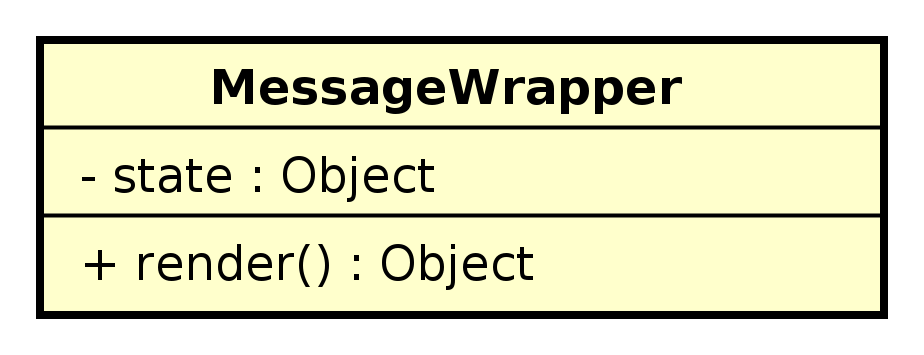
\includegraphics[width=0.3\textwidth]{./img/MessageWrapper.png}
		\caption{Diagramma classe MessageWrapper}
	\end{figure}
	\item \textbf{descrizione:} rappresenta una classe wrapper per visualizzare un messaggio;
	\item \textbf{utilizzo:} viene utilizzato per mostrare messaggi di errore o di successo sulla mappa;
	\item \textbf{attributi:}
	\begin{itemize}
		\item -state : Object\begin{itemize}
			\item rappresenta lo stato del MessageWrapper.\end{itemize}
	\end{itemize}
	\item \textbf{metodi:}
	\begin{itemize}
		\item +render() : Object\newline
		renderizza il MessageWrapper
	\end{itemize}
	\item \textbf{relazioni con altre classi:} 
	\begin{itemize}
		\item IN MapWrapper.
	\end{itemize}
\end{itemize}
\paragraph{PolygonOperationWrapper}
\begin{itemize}
	\begin{figure}[H]
		\centering
		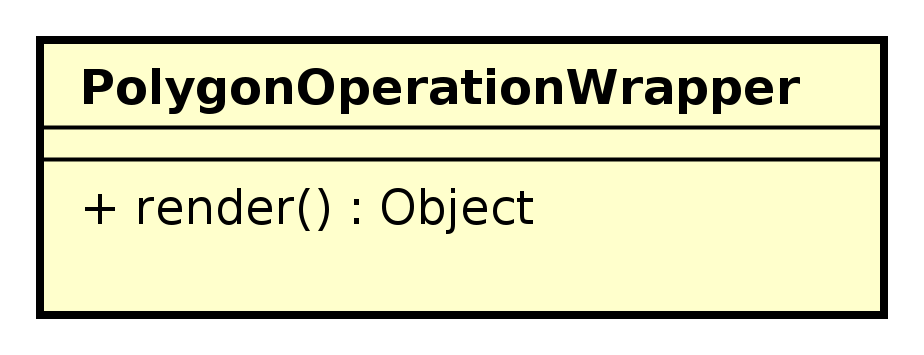
\includegraphics[width=0.3\textwidth]{./img/PolygonOperationWrapper.png}
		\caption{Diagramma classe PolygonOperationWrapper}
	\end{figure}
	\item \textbf{descrizione:} rappresenta una classe wrapper per visualizzare un bottone con cui è possibile effettuare operazioni sul perimetro di un poligono sulla mappa;
	\item \textbf{utilizzo:} invocando i suoi metodi è possibile iniziare a disegnare il poligono su mappa oppure cancellare l'ultimo segmento disegnato;
	\item \textbf{metodi:}
	\begin{itemize}
		\item +render() : Object\newline
		renderizza il PolygonOperationWrapper
	\end{itemize}
	\item \textbf{relazioni con altre classi:} 
	\begin{itemize}
		\item IN MapWrapper;
		\item OUT MapWrapper.
	\end{itemize}
\end{itemize}
\newpage
\subsection{DeGeOP::ViewPkg::SidebarPkg}
\label{pkg::SidebarPkg}
\begin{figure}[H]
	\centering
	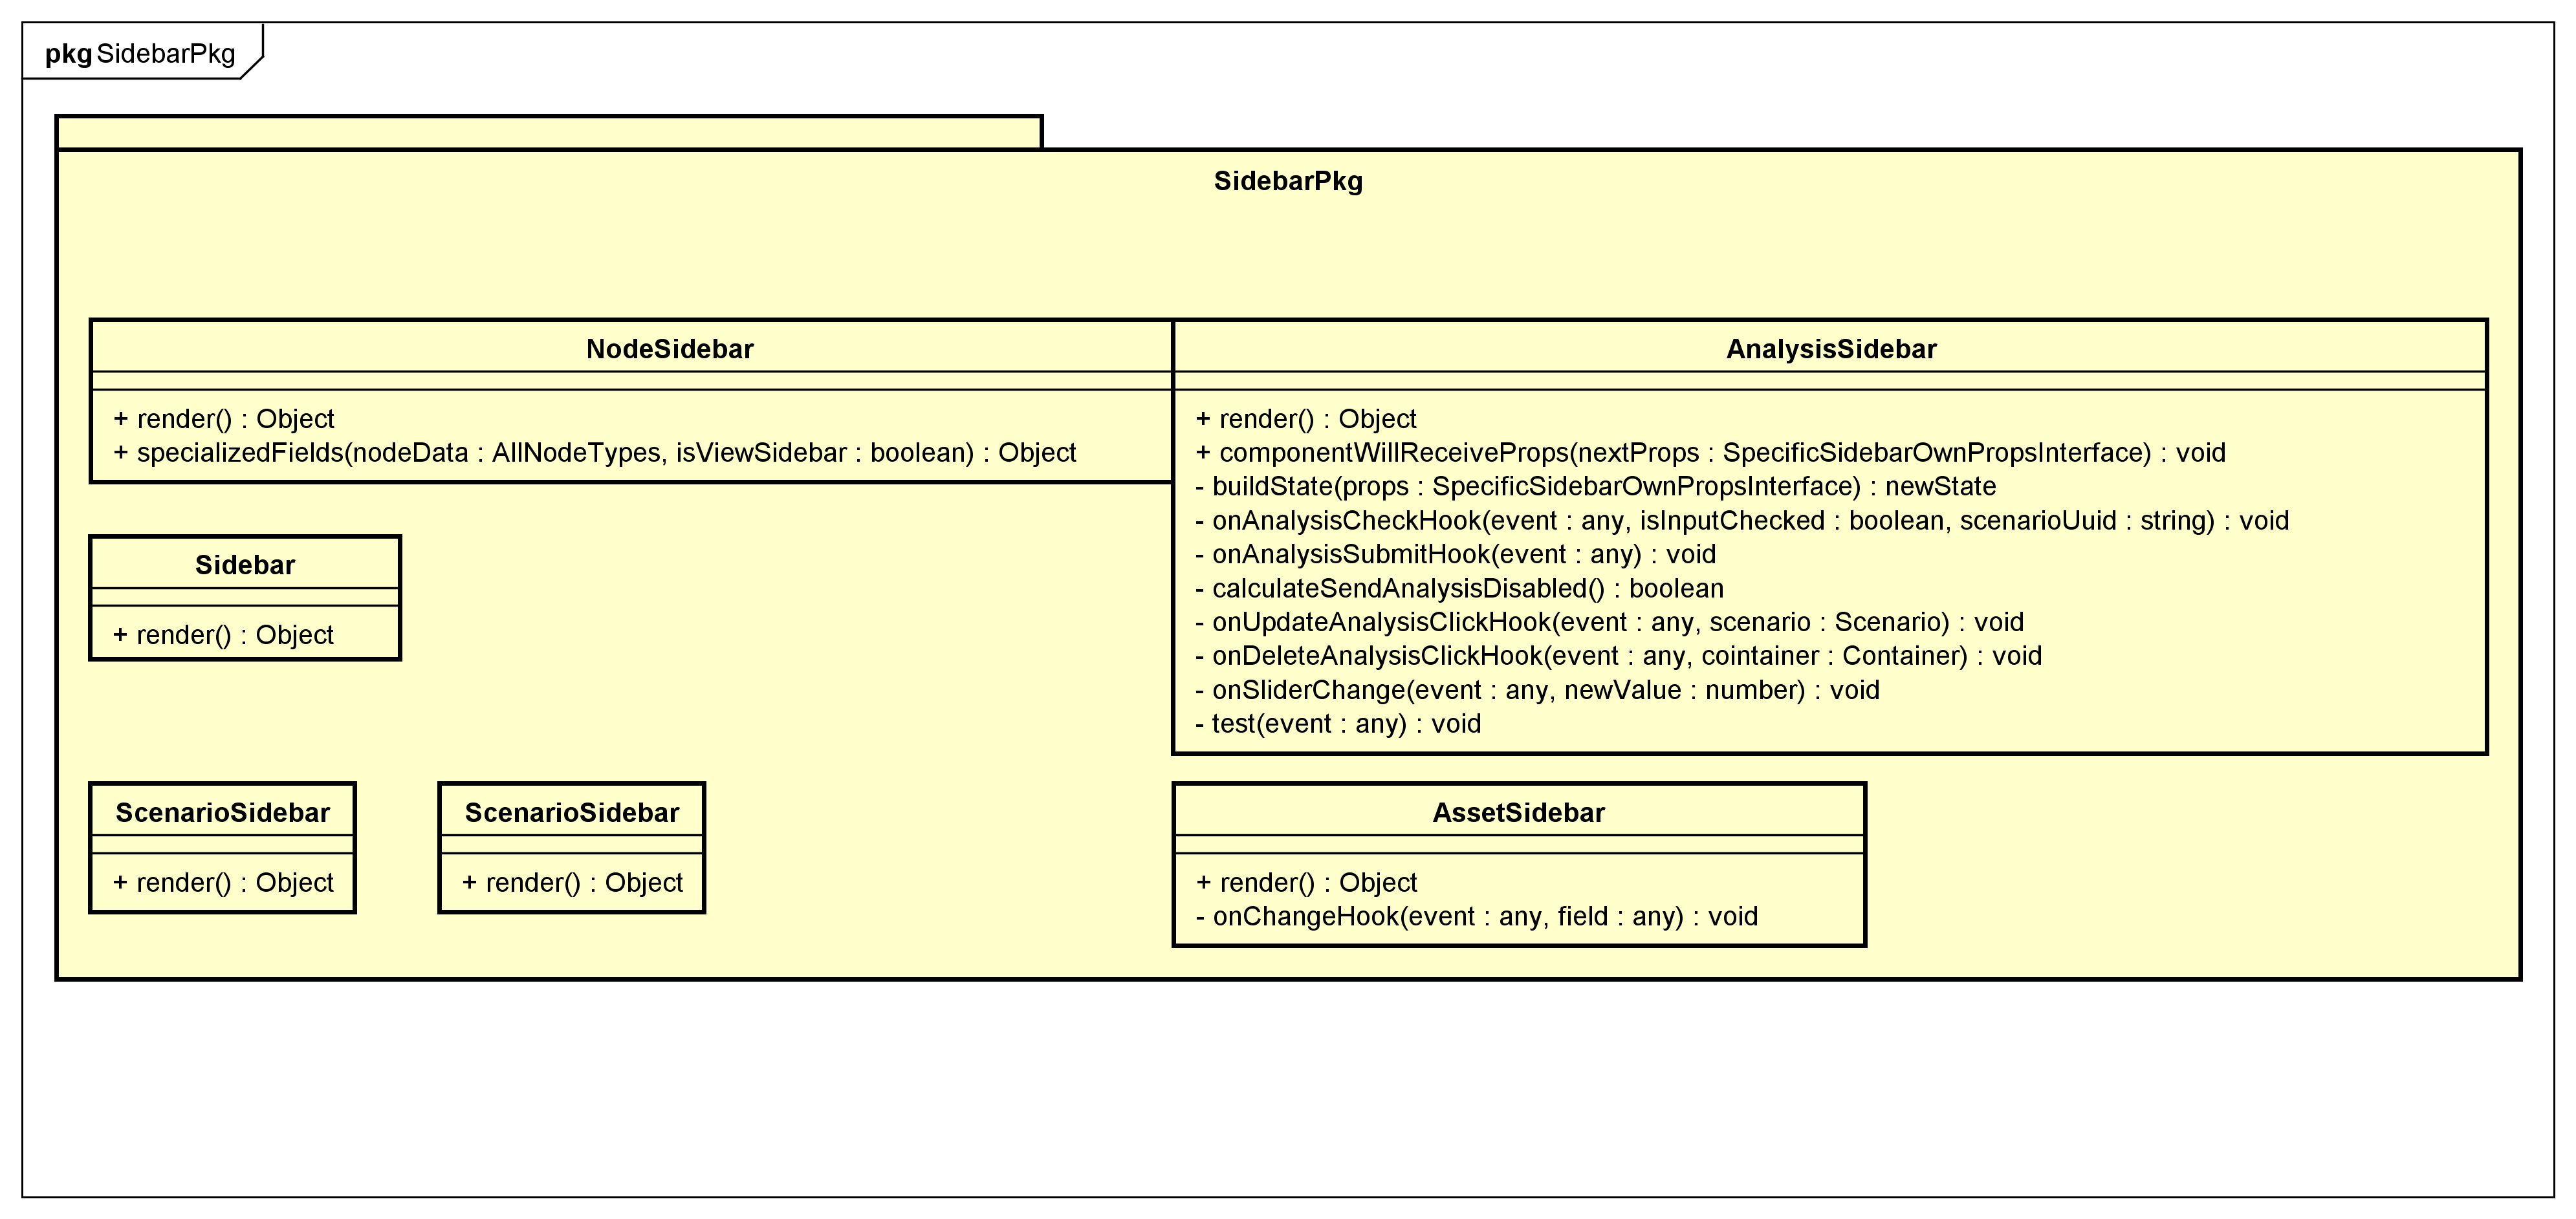
\includegraphics[width=\textwidth]{img/PkgDiagram/SidebarPkg.png}
	\caption{Schema componente DeGeOP::ViewPkg::SidebarPkg}
\end{figure}
\subsubsection{Informazioni sul package}
\begin{itemize}
	\item \textbf{descrizione:} racchiude le componenti necessarie alla rappresentazione della sidebar;
	\item \textbf{padre:} \hyperref[pkg::ViewPkg]{ViewPkg};
	\item \textbf{package contenuti:}
	\begin{itemize}
		\item SidebarPkg::\hyperref[pkg::ButtonsPkg]{ButtonsPkg};
		\item SidebarPkg::\hyperref[pkg::ContentPkg]{ContentPkg}.
	\end{itemize}
	\item \textbf{interazioni con altri package:} 
	\begin{itemize}
		\item IN DeGeOPViewPkg: utilizzo della sidebar.
	\end{itemize}
	\item \textbf{classi contenute:}
	\begin{itemize}
		\item AnalysisSidebar;
		\item AssetSidebar;
		\item EdgeSidebar;
		\item NodeSidebar;
		\item ScenarioSidebar.
	\end{itemize}
\end{itemize}
\subsubsection{Classi}
\paragraph{AnalysisSidebar}
\begin{itemize}
	\item \textbf{descrizione:} rappresenta una sidebar relativo all'analisi di uno scenario;
	\item \textbf{utilizzo:} renderizza una sidebar composta da contenuto in cui l'utente può gestire l'analisi degli scenari;
	\item \textbf{metodi:}
	\begin{itemize}
		\item +buildState(props) : newState\newline
		costruisce il nuovo stato
		\begin{itemize}
			\item props : SpecificSidebarOwnPropsInterface\\
			indica le props dello stato.
		\end{itemize}
		\item +calculateSendAnalysisDisabled() : boolean\newline
		restituisce false solamente se è selezionata almeno un'analisi
		\item +componentWillReceiveProps(nextProps) : void\newline
		imposta nello state la lista di scenari non analizzati
		\begin{itemize}
			\item nextProps : SpecificSidebarOwnPropsInterface\\
			rappresenta le props con le quali lo state dev'essere aggiornato.
		\end{itemize}
		\item +onAnalysisCheckHook(event, isInputChecked, scenarioUuid) : newState\newline
		gestisce il cambiamento dell'input all'interno di un checkbox
		\begin{itemize}
			\item event : any\\
			rappresenta l'evento da gestire.
			\item isInputChecked : boolean\\
			restituisce true solamente se lo scenario è selezionato.
			\item scenarioUuid : string\\
			indica l'uuid dello scenario.
		\end{itemize}
		\item +onAnalysisSubmitHook(event) : void\newline
		gestisce il cambiamento alla sottomissione dell'analisi
		\begin{itemize}
			\item event : any\\
			rappresenta l'evento da gestire.
		\end{itemize}
		\item +onDeleteAnalysisClickHook(container, event) : void\newline
		gestisce il cambiamento a seguito dell'eliminazione di uno scenario dall'analisi
		\begin{itemize}
			\item container : Container\\
			rappresenta il container attuale dell'analisi.
			\item event : any\\
			rappresenta l'evento da gestire.
		\end{itemize}
		\item +onSliderChange(event, newValue) : void\newline
		gestisce il cambiamento dello slider
		\begin{itemize}
			\item event : any\\
			indica l'evento da gestire.
			\item newValue : number\\
			indica il nuovo valore da assegnare allo slider.
		\end{itemize}
		\item +onUpdateAnalysisClickHook(event, scenario) : void\newline
		gestisce il cambiamento a seguito dell'aggiornamento dell'analisi
		
		\begin{itemize}
			\item event : any\\
			indica l'evento da gestire.
			\item scenario : Scenario\\
			rappresenta lo scenario da gestire.
		\end{itemize}
		\item +render() : Object\newline
		il metodo renderizza la sidebar contenente i campi dati per l'analisi degli scenari
		
		\item +test(event) : void\newline
		metodo di prova per il calcolo del risultato globale
		\begin{itemize}
			\item event : any\\
			rappresenta l'evento da gestire.
		\end{itemize}
	\end{itemize}
\end{itemize}
\paragraph{AssetSidebar}
\begin{itemize}
	\item \textbf{descrizione:} rappresenta una sidebar per l'inserimento e la modifica di un asset;
	\item \textbf{utilizzo:} renderizza una sidebar composta da contenuto in cui l'utente può compilare i dati per l'inserimento e la modifica relative ad un asset;
	\item \textbf{metodi:}
	\begin{itemize}
		\item +onChangeHook(event, field) : void\newline
		gestisce il cambiamento dell'input all'interno di un inputbox
		\begin{itemize}
			\item event : any\\
			indica l'evento da gestire.
			\item field : any\\
			indica il campo su cui è accaduto l'evento.
		\end{itemize}
		\item +render() : Object\newline
		rappresenta una sidebar per l'inserimento e la modifica di un asset
	\end{itemize}
\end{itemize}
\paragraph{EdgeSidebar}
\begin{itemize}
	\item \textbf{descrizione:} rappresenta una sidebar per l'inserimento e la modifica di un arco;
	\item \textbf{utilizzo:} renderizza una sidebar composta da contenuto in cui l'utente può compilare i dati per l'inserimento e la modifica di un arco;
	\item \textbf{metodi:}
	\begin{itemize}
		\item +render() : Object\newline
		il metodo renderizza la sidebar contenente i campi dati per l'inserimento e la modifica di un edge
	\end{itemize}
\end{itemize}
\paragraph{NodeSidebar}
\begin{itemize}
	\item \textbf{descrizione:} rappresenta una sidebar per l'inserimento e la modifica di un nodo;
	\item \textbf{utilizzo:} renderizza una sidebar composta da contenuto in cui l'utente può compilare i dati per l'inserimento e la modifica relative ad un nodo;
	\item \textbf{metodi:}
	\begin{itemize}
		\item +render() : Object\newline
		il metodo renderizza la sidebar  contenente i campi dati per l'inserimento e la modifica di un nodo
		
		\item +specializedFields(isViewSidebar, nodeData) : Object\newline
		Ritorna i campi specifici che cambiano in base al tipo di nodo selezionato
		\begin{itemize}
			\item isViewSidebar : boolean\\
			il valore è true solamente se si tratta della sidebar relativa alla view.
			\item nodeData : AllNodeTypes\\
			contiene i dati relativi al nodo.
		\end{itemize}
	\end{itemize}
\end{itemize}
\paragraph{ScenarioSidebar}
\begin{itemize}
	\item \textbf{descrizione:} rappresenta una sidebar per l'inserimento e la modifica di uno scenario;
	\item \textbf{utilizzo:} renderizza una sidebar composta da contenuto in cui l'utente può compilare i dati per l'inserimento e la modifica relative ad uno scenario;
	\item \textbf{metodi:}
	\begin{itemize}
		\item +getScenariosMenuItems() : Object\newline
		ritorna le liste dei MenuItem degli scenari da visualizzare
		\item +onScenarioChangeHook(event, index, value) : void\newline
		gestisce il cambiamento dell'input per la scelta dello scenario
		\begin{itemize}
			\item event : any\\
			rappresenta l'evento relativo alla scelta dello scenario.
			\item index : any\\
			indica l'indice appartenente allo scenario scelto.
			\item value : any\\
			rappresenta lo scenario selezionato.
		\end{itemize}
		\item +render() : Object\newline
		il metodo renderizza la sidebar contenente i campi dati per l'inserimento e la modifica di uno scenario
	\end{itemize}
\end{itemize}
\newpage
\subsection{DeGeOP::ViewPkg::SidebarPkg::ButtonsPkg}
\label{pkg::ButtonsPkg}
\begin{figure}[H]
	\centering
	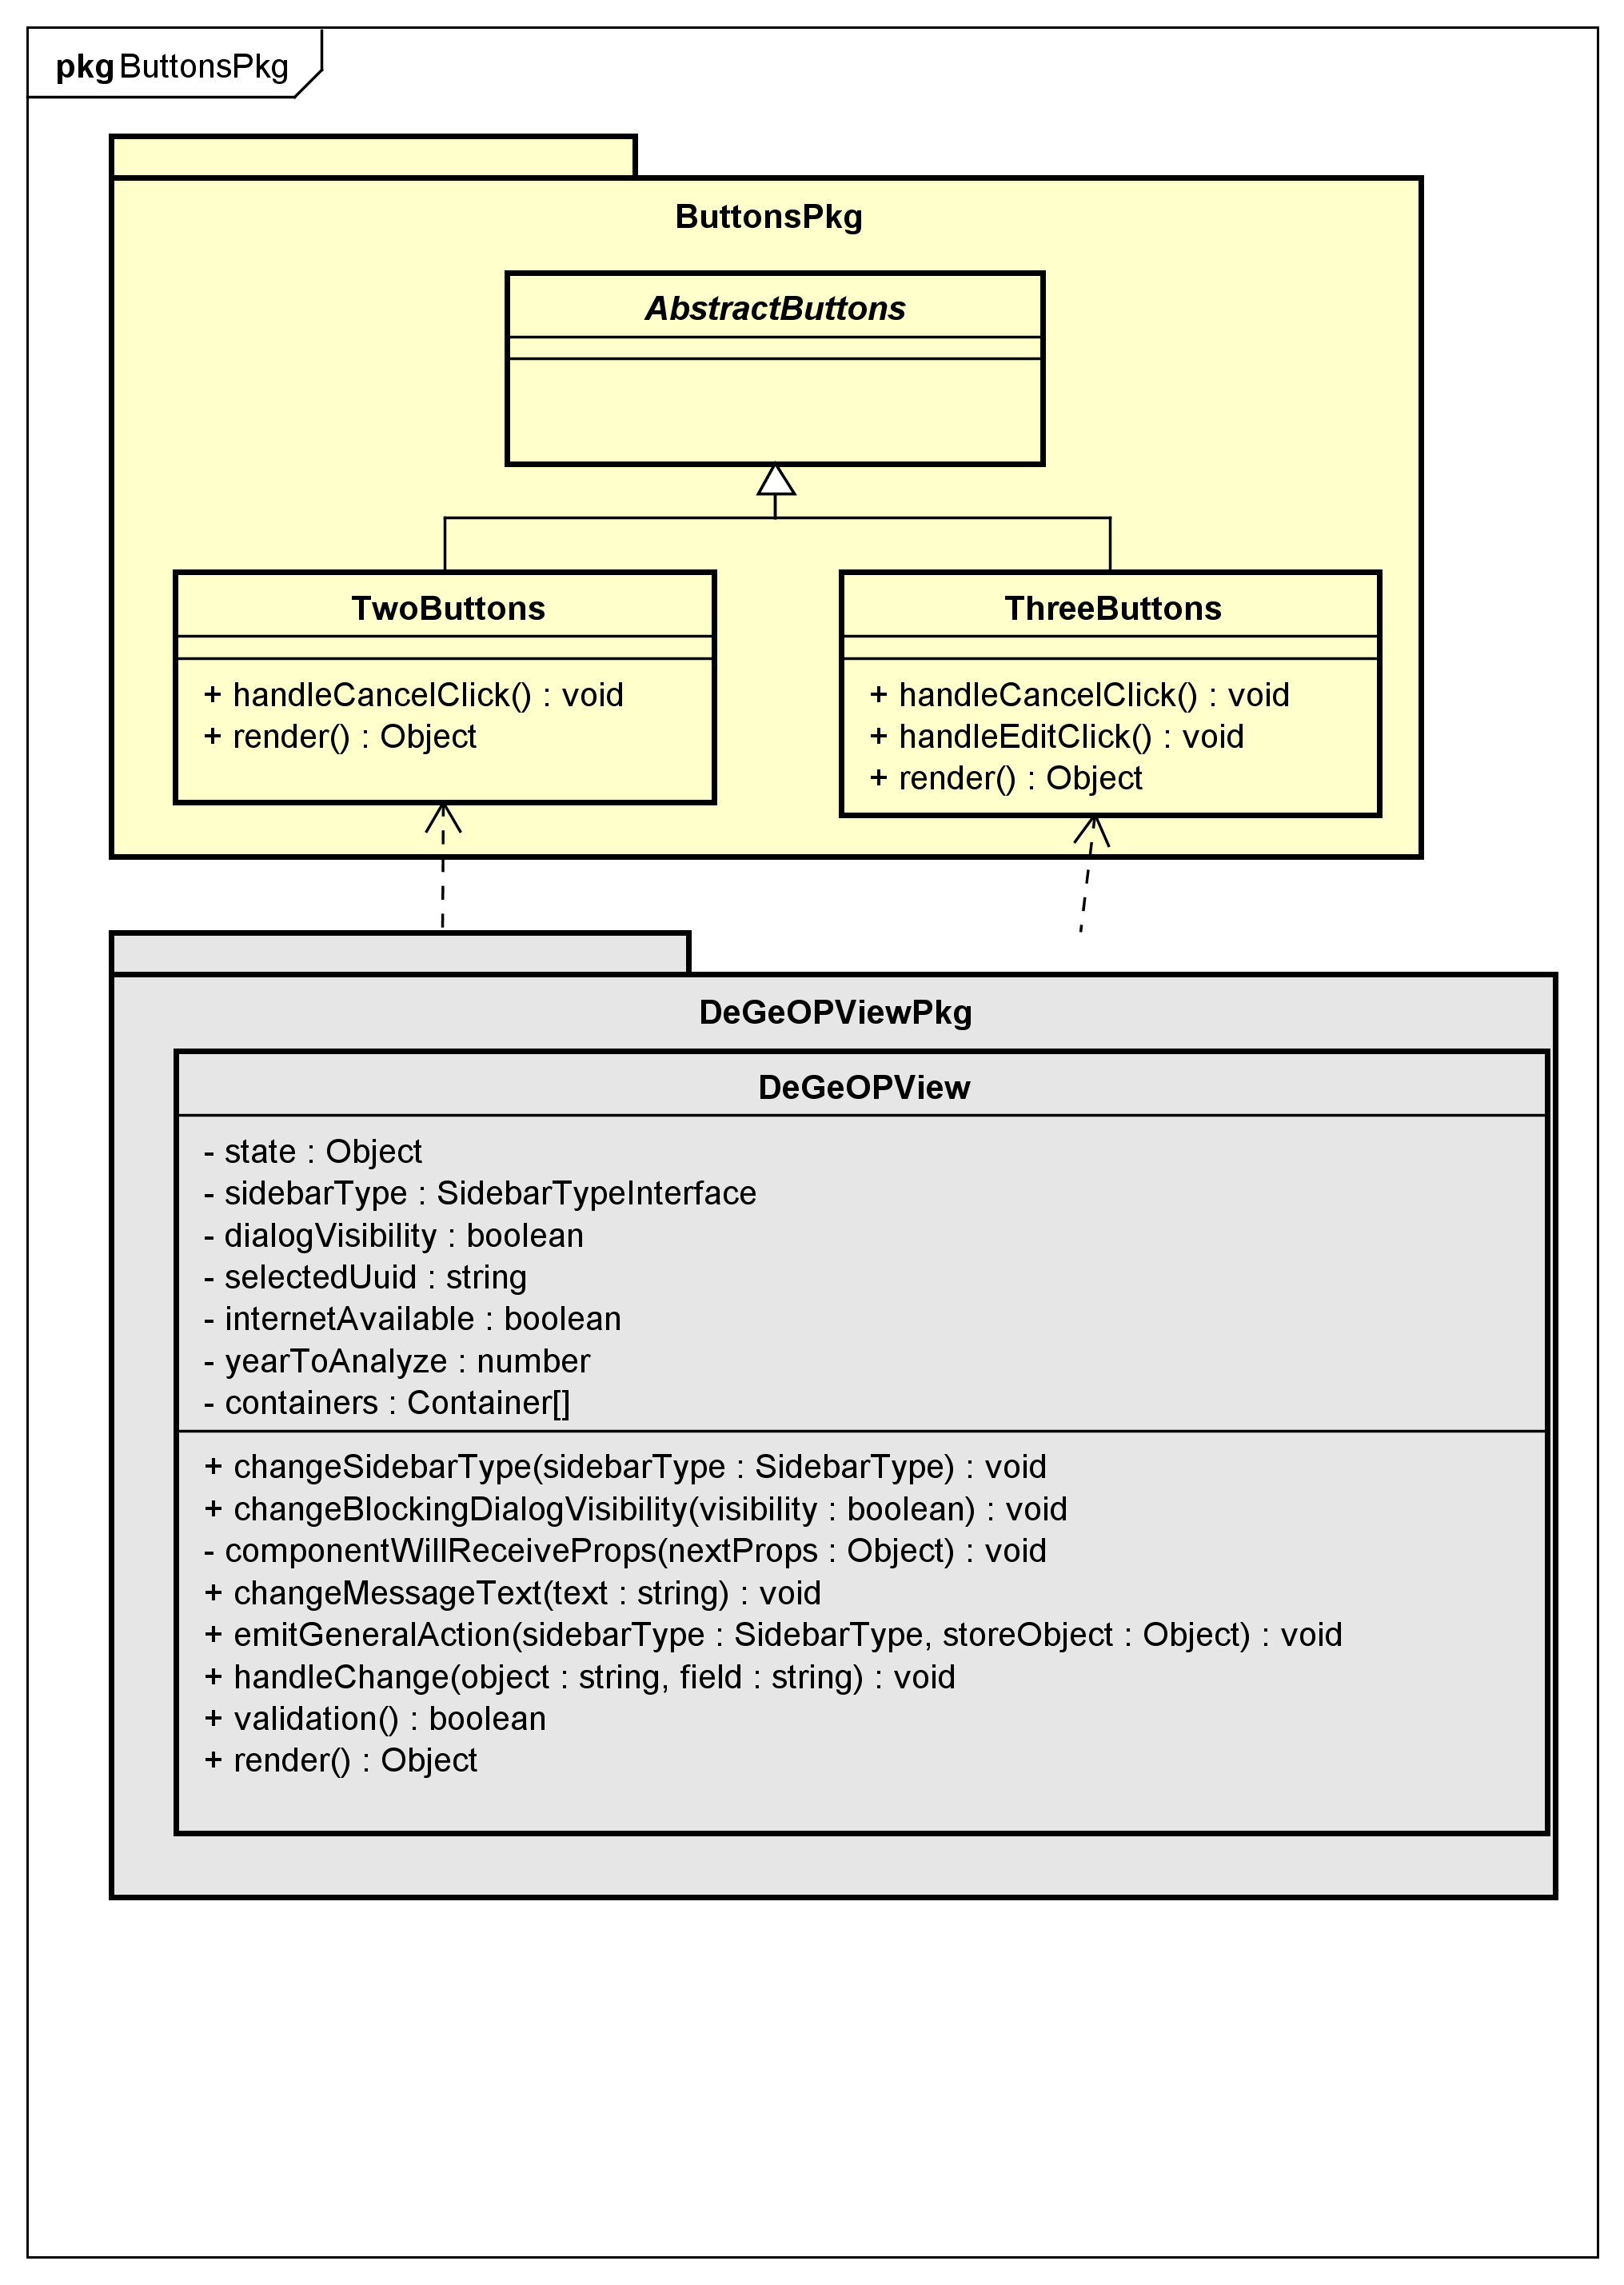
\includegraphics[width=\textwidth]{img/PkgDiagram/ButtonsPkg.png}
	\caption{Schema componente DeGeOP::ViewPkg::SidebarPkg::ButtonsPkg}
\end{figure}
\subsubsection{Informazioni sul package}
\begin{itemize}
	\item \textbf{descrizione:} racchiude le componenti che sono relative all'area con i bottoni della Sidebar;
	\item \textbf{padre:} \hyperref[pkg::SidebarPkg]{SidebarPkg};
	\item \textbf{classi contenute:}
	\begin{itemize}
		\item AbstractButtons;
		\item ThreeButtons;
		\item TwoButtons.
	\end{itemize}
\end{itemize}
\subsubsection{Classi}
\paragraph{AbstractButtons}
\begin{itemize}
	\begin{figure}[H]
		\centering
		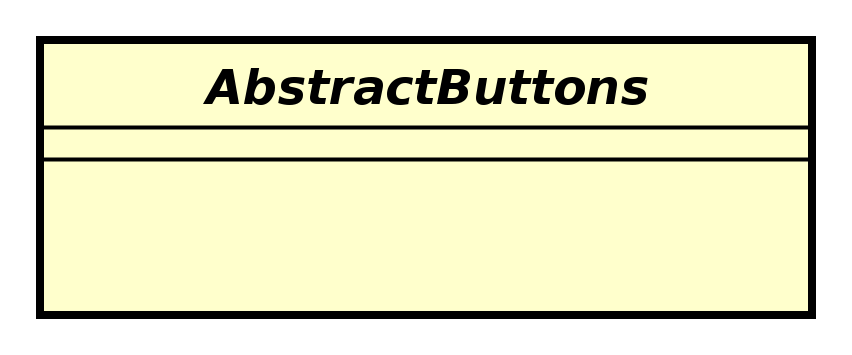
\includegraphics[width=0.3\textwidth]{./img/AbstractButtons.png}
		\caption{Diagramma classe AbstractButtons}
	\end{figure}
	\item \textbf{descrizione:} una classe d'interfaccia rappresentante i bottoni inseriti nella sidebar;
	\item \textbf{utilizzo:} viene riferita da sidebar in quanto è una delle sue componenti.
\end{itemize}
\paragraph{ThreeButtons}
\begin{itemize}
	\begin{figure}[H]
		\centering
		\includegraphics[width=0.3\textwidth]{./img/ThreeButtons.png}
		\caption{Diagramma classe ThreeButtons}
	\end{figure}
	\item \textbf{descrizione:} classe che renderizza tre bottoni, uno di modifica,  uno di eliminazione e uno di annullamento. Il bottone di annullamento provoca l'annullamento della selezione corrente. Il bottone di eliminazione provoca la comparsa di una finestra modale che chiede la conferma dell'eliminazione dell'elemento correntemente selezionato. Il bottone di modifica provoca l'avvio della modalità di modifica, con cui è possibile ridisegnare l'asset o cambiare i campi dati;
	\item \textbf{utilizzo:} viene utilizzata nelle sidebar di visualizzazione;
	\item \textbf{metodi:}
	\begin{itemize}
		\item +handleCancelClick() : void\newline
		il metodo gestisce il click sul bottone di annullamento, ripristinando la sidebar di default
		\item +handleEditClick() : void\newline
		il metodo imposta la sidebar di modifica dell'elemento attualmente selezionato
		\item +render() : Object\newline
		renderizza tre bottoni, uno di modifica, uno di annullamento e uno di eliminazione
	\end{itemize}
\end{itemize}
\paragraph{TwoButtons}
\begin{itemize}
	\begin{figure}[H]
		\centering
		\includegraphics[width=0.3\textwidth]{./img/TwoButtons.png}
		\caption{Diagramma classe TwoButtons}
	\end{figure}
	\item \textbf{descrizione:} classe che renderizza due bottoni, uno di salvataggio e uno di annullamento. Il bottone di salvataggio è disabilitato fino a che tutti i campi della sidebar non sono stati compilati in modo corretto. Il bottone di annullamento provoca l'interruzione dell'inserimento dei dati;
	\item \textbf{utilizzo:} viene utilizzata nelle sidebar di inserimento;
	\item \textbf{metodi:}
	\begin{itemize}
		\item +handleCancelClick() : void\newline
		il metodo gestisce il click sul bottone di annullamento, ripristinando la sidebar di default
		\item +render() : Object\newline
		renderizza due bottoni, uno di annullamento e uno di salvataggio
	\end{itemize}
\end{itemize}
\newpage

	%\newpage

\section{Diagrammi di sequenza}
	\newpage
\section{Tracciamento}

\subsection{Tracciamento classi-requisiti}
% v: 1
\def\arraystretch{1.5}
\rowcolors{2}{D}{P}
\begin{longtable}{p{5cm}!{\VRule[1pt]}p{2.5cm}}
	\rowcolor{I}
	\color{white} \textbf{Classe} & \color{white} \textbf{Requisito} \\ 
	\endfirsthead
	\rowcolor{I}
	\color{white} \textbf{Classe} & \color{white} \textbf{Requisito} \\ 
	\endhead
	Asset & ROF1 \newline ROF1.3 \newline ROF1.4 \newline ROF1.5 \newline ROF2 \newline ROF4 \newline ROF4.4 \newline ROF5\\
	AssetAction & ROF1 \newline ROF1.5 \newline ROF4 \newline ROF4.4 \newline ROF5\\
	AssetActionCreator & ROF1 \newline ROF1.5 \newline ROF4 \newline ROF4.4 \newline ROF5 \newline ROF5.1 \newline ROF6.10\\
	AssetReducer & ROF1 \newline ROF1.5 \newline ROF4 \newline ROF4.4 \newline ROF5 \newline ROF5.1 \newline ROF6.10\\
	ButtonWrapper & RFF16 \newline RFF19.1.9 \newline ROF1 \newline ROF1.3 \newline ROF1.4 \newline ROF10 \newline ROF11 \newline ROF14 \newline ROF15 \newline ROF4 \newline ROF4.3 \newline ROF5 \newline ROF6 \newline ROF9 \newline ROF9.2 \newline ROF9.9\\
	ConcretePolygon & ROF1.3 \newline ROF1.4\\
	ConcretePolygonFactory & RFF16 \newline RFF19 \newline ROF1 \newline ROF4\\
	Coordinate & ROF1.3 \newline ROF1.4\\
	Customer & RFF16 \newline RFF20 \newline RFF47 \newline RFF48 \newline RFF48.1 \newline ROF1 \newline ROF1.3 \newline ROF1.4 \newline ROF1.5 \newline ROF10 \newline ROF11 \newline ROF14 \newline ROF15 \newline ROF4 \newline ROF5 \newline ROF6 \newline ROF9\\
	DataToServer & RFF16 \newline RFF19 \newline RFF20 \newline RFF21 \newline ROF1 \newline ROF1.5 \newline ROF10 \newline ROF11 \newline ROF14 \newline ROF15 \newline ROF4 \newline ROF5 \newline ROF6 \newline ROF9\\
	DeGeOPView & RFF16 \newline RFF19.4 \newline RFF21 \newline RFF24.4 \newline RFF25 \newline RFF25.1 \newline RFF26 \newline RFF26.1 \newline RFF47 \newline RFF48 \newline ROF1 \newline ROF1.3 \newline ROF1.4 \newline ROF1.5 \newline ROF10 \newline ROF11 \newline ROF14 \newline ROF15 \newline ROF24 \newline ROF24.1 \newline ROF24.2 \newline ROF24.3 \newline ROF39 \newline ROF4 \newline ROF4.1.1 \newline ROF4.1.2 \newline ROF4.1.3 \newline ROF4.2 \newline ROF4.3 \newline ROF4.5 \newline ROF40 \newline ROF41 \newline ROF5 \newline ROF6 \newline ROF6.11 \newline ROF9 \newline ROF9.2 \newline ROF9.9\\
	Edge & ROF1.3 \newline ROF1.4 \newline ROF10 \newline ROF11 \newline ROF12 \newline ROF14 \newline ROF15 \newline ROF5\\
	EdgeAction & ROF11 \newline ROF14 \newline ROF15\\
	EdgeActionCreator & RFF14.5 \newline ROF11 \newline ROF14 \newline ROF14.7 \newline ROF15 \newline ROF15.1\\
	EdgeReducer & RFF14.5 \newline ROF11 \newline ROF11.5 \newline ROF14 \newline ROF14.1 \newline ROF14.2 \newline ROF15 \newline ROF15.1\\
	ExitNode & ROF1.3 \newline ROF1.4 \newline ROF10 \newline ROF5\\
	InsertAssetContent & ROF1.2 \newline ROF1.2.1 \newline ROF1.2.1.1 \newline ROF1.2.2 \newline ROF1.2.2.1 \newline ROF1.2.3 \newline ROF1.2.3.1 \newline ROF1.2.3.2 \newline ROF1.2.3.3 \newline ROF1.2.3.4 \newline ROF1.2.3.5 \newline ROF1.2.3.6 \newline ROF1.2.4 \newline ROF1.2.4.1 \newline ROF1.2.4.2 \newline ROF1.2.4.3 \newline ROF1.2.4.4 \newline ROF1.2.5 \newline ROF1.2.5.1 \newline ROF1.2.5.2 \newline ROF1.2.6 \newline ROF1.2.6.1 \newline ROF1.2.7 \newline ROF1.2.7.1 \newline ROF1.6\\
	InsertEdgeContent & RFF11.2 \newline RFF11.3 \newline RFF11.3.1 \newline RFF11.3.1.1 \newline RFF11.3.2 \newline RFF11.6 \newline RFF11.7 \newline ROF1.6 \newline ROF11.3.2.1 \newline ROF11.4\\
	InsertNodeContent & ROF6.1 \newline ROF6.12 \newline ROF6.12.1 \newline ROF6.12.1.1 \newline ROF6.3 \newline ROF6.3.1 \newline ROF6.3.2 \newline ROF6.3.3 \newline ROF6.3.4 \newline ROF6.3.5 \newline ROF6.3.6 \newline ROF6.4 \newline ROF6.5 \newline ROF6.5.2 \newline ROF6.5.2.1 \newline ROF6.5.3 \newline ROF6.5.3.1 \newline ROF6.5.4 \newline ROF6.5.4.1 \newline ROF6.6 \newline ROF6.6.2 \newline ROF6.6.2.1 \newline ROF6.7 \newline ROF6.7.2 \newline ROF6.7.2.1 \newline ROF6.8 \newline ROF9.1\\
	MachineNode & ROF1.3 \newline ROF1.4 \newline ROF10 \newline ROF5\\
	MapWrapper & RFF16 \newline RFF16.1.10 \newline RFF16.1.7 \newline RFF16.1.7.1 \newline RFF16.1.8 \newline RFF16.1.8.1 \newline RFF16.1.9 \newline RFF16.2 \newline RFF16.3 \newline RFF19.1.10 \newline RFF19.1.7 \newline RFF19.1.7.1 \newline RFF19.1.8 \newline RFF19.1.8.1 \newline RFF19.1.9 \newline RFF24.4 \newline ROF1 \newline ROF1.1 \newline ROF1.1.1 \newline ROF1.1.2 \newline ROF1.1.3 \newline ROF1.3 \newline ROF1.5 \newline ROF10 \newline ROF11 \newline ROF11.1 \newline ROF11.1.1 \newline ROF11.1.2 \newline ROF14 \newline ROF15 \newline ROF24 \newline ROF24.1 \newline ROF24.2 \newline ROF24.3 \newline ROF4 \newline ROF4.1 \newline ROF4.3 \newline ROF42 \newline ROF43 \newline ROF44 \newline ROF5 \newline ROF6 \newline ROF6.1 \newline ROF6.2 \newline ROF9 \newline ROF9.1 \newline ROF9.1.1 \newline ROF9.1.3 \newline ROF9.2 \newline ROF9.9\\
	MessageWrapper & RFF14.8 \newline RFF16 \newline RFF16.4 \newline RFF19.4 \newline RFF20 \newline RFF22 \newline RFF23 \newline RFF47 \newline RFF48 \newline ROF1 \newline ROF1.3 \newline ROF1.5 \newline ROF1.6 \newline ROF10 \newline ROF11 \newline ROF14 \newline ROF15 \newline ROF15.1 \newline ROF15.2 \newline ROF20.1 \newline ROF4 \newline ROF4.3 \newline ROF4.5 \newline ROF5 \newline ROF6 \newline ROF6.11 \newline ROF9 \newline ROF9.11 \newline ROF9.2 \newline ROF9.9\\
	Node & ROF1.3 \newline ROF1.4 \newline ROF10 \newline ROF6 \newline ROF7 \newline ROF9 \newline ROF9.10\\
	NodeAction & ROF10 \newline ROF6 \newline ROF9 \newline ROF9.10\\
	NodeActionCreator & ROF10 \newline ROF10.1 \newline ROF6 \newline ROF9 \newline ROF9.10\\
	NodeReducer & ROF10 \newline ROF10.1 \newline ROF6 \newline ROF9 \newline ROF9.10\\
	Polygon & RFF16 \newline RFF19 \newline ROF1 \newline ROF1.5 \newline ROF10 \newline ROF15 \newline ROF4 \newline ROF5\\
	PolygonFactory & RFF19\\
	PolygonOperationWrapper & RFF16 \newline RFF16.1.10 \newline RFF16.1.7.1 \newline RFF16.1.8 \newline RFF16.1.8.1 \newline RFF16.1.9 \newline RFF19.1.7 \newline RFF19.1.8 \newline ROF1 \newline ROF1.1 \newline ROF1.1.2 \newline ROF1.5 \newline ROF10 \newline ROF15 \newline ROF20.2 \newline ROF4 \newline ROF4.1 \newline ROF5\\
	Process & ROF1.3 \newline ROF1.4 \newline ROF10 \newline ROF15 \newline ROF5\\
	QueueNode & ROF1.3 \newline ROF1.4 \newline ROF10 \newline ROF15 \newline ROF5\\
	Reducer & RFF14.5 \newline RFF16 \newline ROF1 \newline ROF1.5 \newline ROF10 \newline ROF10.1 \newline ROF11 \newline ROF11.5 \newline ROF14 \newline ROF14.1 \newline ROF14.2 \newline ROF15 \newline ROF15.1 \newline ROF4 \newline ROF5 \newline ROF5.1 \newline ROF6 \newline ROF6.10 \newline ROF9\\
	ResourceNode & ROF1.3 \newline ROF1.4 \newline ROF10 \newline ROF15 \newline ROF5\\
	Sidebar & RFF16 \newline ROF1 \newline ROF1.3 \newline ROF1.4 \newline ROF1.5 \newline ROF10 \newline ROF11 \newline ROF14 \newline ROF15 \newline ROF4 \newline ROF4.3 \newline ROF5 \newline ROF6 \newline ROF9 \newline ROF9.2 \newline ROF9.9\\
	SourceNode & ROF1.3 \newline ROF1.4 \newline ROF10 \newline ROF15 \newline ROF5\\
	StoreDeGeOP & RFF20 \newline RFF25 \newline RFF25.1 \newline RFF26 \newline RFF26.1 \newline RFF47 \newline RFF48 \newline RFF48.1 \newline ROF1.3 \newline ROF1.4 \newline ROF10 \newline ROF10.1 \newline ROF11.5 \newline ROF14.1 \newline ROF14.2 \newline ROF15 \newline ROF5 \newline ROF5.1 \newline ROF6.10\\
	ViewAssetContent & ROF2 \newline ROF3 \newline ROF42 \newline ROF5.2 \newline ROF6.10\\
	ViewEdgeContent & ROF12 \newline ROF13 \newline ROF44\\
	ViewNodeContent & ROF10.2 \newline ROF43 \newline ROF7 \newline ROF8\\
	\rowcolor{white}
	\caption{Tracciamento classe-requisiti}
\end{longtable}

\subsection{Tracciamento requisiti-classi}
% v: 1
\def\arraystretch{1.5}
\rowcolors{2}{D}{P}
\begin{longtable}{p{2.5cm}!{\VRule[1pt]}p{5cm}}
	\rowcolor{I}
	\color{white} \textbf{Requisito} & \color{white} \textbf{Classe} \\ 
	\endfirsthead
	\rowcolor{I}
	\color{white} \textbf{Requisito} & \color{white} \textbf{Classe} \\ 
	\endhead
	RFF11.2 & InsertEdgeContent\\
	RFF11.3 & InsertEdgeContent\\
	RFF11.3.1 & InsertEdgeContent\\
	RFF11.3.1.1 & InsertEdgeContent\\
	RFF11.3.2 & InsertEdgeContent\\
	RFF11.6 & InsertEdgeContent\\
	RFF11.7 & InsertEdgeContent\\
	RFF14.4 & Non implementato\\
	RFF14.5 & EdgeActionCreator \newline EdgeReducer \newline Reducer\\
	RFF14.5.1 & Non implementato \\
	RFF14.5.1.1 & Non implementato\\
	RFF14.5.2 & Non implementato\\
	RFF14.5.2.1 & Non implementato\\
	RFF14.8 & MessageWrapper\\
	RFF16 & ButtonWrapper \newline ConcretePolygonFactory \newline Customer \newline DataToServer \newline DeGeOPView \newline MapWrapper \newline MessageWrapper \newline Polygon \newline PolygonOperationWrapper \newline Reducer \newline Sidebar\\
	RFF16.1 & Non implementato\\
	RFF16.1.1 & Non implementato\\
	RFF16.1.1.1 & Non implementato\\
	RFF16.1.10 & MapWrapper \newline PolygonOperationWrapper\\
	RFF16.1.11 & Non implementato\\
	RFF16.1.2 & Non implementato\\
	RFF16.1.2.1 & Non implementato\\
	RFF16.1.3 & Non implementato\\
	RFF16.1.3.1 & Non implementato\\
	RFF16.1.3.10 & Non implementato\\
	RFF16.1.3.11 & Non implementato\\
	RFF16.1.3.2 & Non implementato\\
	RFF16.1.3.3 & Non implementato\\
	RFF16.1.3.4 & Non implementato\\
	RFF16.1.3.5 & Non implementato\\
	RFF16.1.3.6 & Non implementato\\
	RFF16.1.3.7 & Non implementato\\
	RFF16.1.3.8 & Non implementato\\
	RFF16.1.3.9 & Non implementato\\
	RFF16.1.4 & Non implementato\\
	RFF16.1.4.1 & Non implementato\\
	RFF16.1.5 & Non implementato\\
	RFF16.1.5.1 & Non implementato\\
	RFF16.1.6 & Non implementato\\
	RFF16.1.6.1 & Non implementato\\
	RFF16.1.7 & MapWrapper\\
	RFF16.1.7.1 & MapWrapper \newline PolygonOperationWrapper\\
	RFF16.1.8 & MapWrapper \newline PolygonOperationWrapper\\
	RFF16.1.8.1 & MapWrapper \newline PolygonOperationWrapper\\
	RFF16.1.9 & MapWrapper \newline PolygonOperationWrapper\\
	RFF16.2 & MapWrapper\\
	RFF16.3 & MapWrapper\\
	RFF16.4 & MessageWrapper\\
	RFF17 & Non implementato\\
	RFF18 & Non implementato\\
	RFF19 & ConcretePolygonFactory \newline DataToServer \newline Polygon \newline PolygonFactory\\
	RFF19.1 & Non implementato\\
	RFF19.1.1 & Non implementato\\
	RFF19.1.1.1 & Non implementato\\
	RFF19.1.10 & MapWrapper\\
	RFF19.1.11 & Non implementato\\
	RFF19.1.2 & Non implementato\\
	RFF19.1.2.1 & Non implementato\\
	RFF19.1.3 & Non implementato\\
	RFF19.1.3.11 & Non implementato\\
	RFF19.1.4 & Non implementato\\
	RFF19.1.4.1 & Non implementato\\
	RFF19.1.5 & Non implementato\\
	RFF19.1.5.1 & Non implementato\\
	RFF19.1.6 & Non implementato\\
	RFF19.1.6.1 & Non implementato\\
	RFF19.1.7 & MapWrapper \newline PolygonOperationWrapper\\
	RFF19.1.7.1 & MapWrapper\\
	RFF19.1.8 & MapWrapper \newline PolygonOperationWrapper\\
	RFF19.1.8.1 & MapWrapper\\
	RFF19.1.9 & ButtonWrapper \newline MapWrapper\\
	RFF19.2 & Non implementato\\
	RFF19.3 & Non implementato\\
	RFF19.4 & DeGeOPView \newline MessageWrapper\\
	RFF20 & Customer \newline DataToServer \newline MessageWrapper \newline StoreDeGeOP\\
	RFF21 & DataToServer \newline DeGeOPView\\
	RFF22 & MessageWrapper\\
	RFF23 & MessageWrapper\\
	RFF24.4 & DeGeOPView \newline MapWrapper\\
	RFF25 & DeGeOPView \newline StoreDeGeOP\\
	RFF25.1 & DeGeOPView \newline StoreDeGeOP\\
	RFF26 & DeGeOPView \newline StoreDeGeOP\\
	RFF26.1 & DeGeOPView \newline StoreDeGeOP\\
	RFF45 & Non implementato\\
	RFF46 & Non implementato\\
	RFF47 & Customer \newline DeGeOPView \newline MessageWrapper \newline StoreDeGeOP\\
	RFF48 & Customer \newline DeGeOPView \newline MessageWrapper \newline StoreDeGeOP\\
	RFF48.1 & Customer \newline StoreDeGeOP\\
	ROF1 & Asset \newline AssetAction \newline AssetActionCreator \newline AssetReducer \newline ButtonWrapper \newline ConcretePolygonFactory \newline Customer \newline DataToServer \newline DeGeOPView \newline MapWrapper \newline MessageWrapper \newline Polygon \newline PolygonOperationWrapper \newline Reducer \newline Sidebar\\
	ROF1.1 & MapWrapper \newline PolygonOperationWrapper\\
	ROF1.1.1 & MapWrapper\\
	ROF1.1.2 & MapWrapper \newline PolygonOperationWrapper\\
	ROF1.1.3 & MapWrapper\\
	ROF1.2 & InsertAssetContent\\
	ROF1.2.1 & InsertAssetContent\\
	ROF1.2.1.1 & InsertAssetContent\\
	ROF1.2.2 & InsertAssetContent\\
	ROF1.2.2.1 & InsertAssetContent\\
	ROF1.2.3 & InsertAssetContent\\
	ROF1.2.3.1 & InsertAssetContent\\
	ROF1.2.3.2 & InsertAssetContent\\
	ROF1.2.3.3 & InsertAssetContent\\
	ROF1.2.3.4 & InsertAssetContent\\
	ROF1.2.3.5 & InsertAssetContent\\
	ROF1.2.3.6 & InsertAssetContent\\
	ROF1.2.4 & InsertAssetContent\\
	ROF1.2.4.1 & InsertAssetContent\\
	ROF1.2.4.2 & InsertAssetContent\\
	ROF1.2.4.3 & InsertAssetContent\\
	ROF1.2.4.4 & InsertAssetContent\\
	ROF1.2.5 & InsertAssetContent\\
	ROF1.2.5.1 & InsertAssetContent\\
	ROF1.2.5.2 & InsertAssetContent\\
	ROF1.2.6 & InsertAssetContent\\
	ROF1.2.6.1 & InsertAssetContent\\
	ROF1.2.7 & InsertAssetContent\\
	ROF1.2.7.1 & InsertAssetContent\\
	ROF1.3 & Asset \newline ButtonWrapper \newline ConcretePolygon \newline Coordinate \newline Customer \newline DeGeOPView \newline Edge \newline ExitNode \newline MachineNode \newline MapWrapper \newline MessageWrapper \newline Node \newline Process \newline QueueNode \newline ResourceNode \newline Sidebar \newline SourceNode \newline StoreDeGeOP\\
	ROF1.4 & Asset \newline ButtonWrapper \newline ConcretePolygon \newline Coordinate \newline Customer \newline DeGeOPView \newline Edge \newline ExitNode \newline MachineNode \newline Node \newline Process \newline QueueNode \newline ResourceNode \newline Sidebar \newline SourceNode \newline StoreDeGeOP\\
	ROF1.5 & Asset \newline AssetAction \newline AssetActionCreator \newline AssetReducer \newline Customer \newline DataToServer \newline DeGeOPView \newline MapWrapper \newline MessageWrapper \newline Polygon \newline PolygonOperationWrapper \newline Reducer \newline Sidebar\\
	ROF1.6 & InsertAssetContent \newline InsertEdgeContent \newline MessageWrapper\\
	ROF10 & ButtonWrapper \newline Customer \newline DataToServer \newline DeGeOPView \newline Edge \newline ExitNode \newline MachineNode \newline MapWrapper \newline MessageWrapper \newline Node \newline NodeAction \newline NodeActionCreator \newline NodeReducer \newline Polygon \newline PolygonOperationWrapper \newline Process \newline QueueNode \newline Reducer \newline ResourceNode \newline Sidebar \newline SourceNode \newline StoreDeGeOP\\
	ROF10.1 & NodeActionCreator \newline NodeReducer \newline Reducer \newline StoreDeGeOP\\
	ROF10.2 & ViewNodeContent\\
	ROF11 & ButtonWrapper \newline Customer \newline DataToServer \newline DeGeOPView \newline Edge \newline EdgeAction \newline EdgeActionCreator \newline EdgeReducer \newline MapWrapper \newline MessageWrapper \newline Reducer \newline Sidebar\\
	ROF11.1 & MapWrapper\\
	ROF11.1.1 & MapWrapper\\
	ROF11.1.2 & MapWrapper\\
	ROF11.3.2.1 & InsertEdgeContent\\
	ROF11.4 & InsertEdgeContent\\
	ROF11.5 & EdgeReducer \newline Reducer \newline StoreDeGeOP\\
	ROF12 & Edge \newline ViewEdgeContent\\
	ROF13 & ViewEdgeContent\\
	ROF14 & ButtonWrapper \newline Customer \newline DataToServer \newline DeGeOPView \newline Edge \newline EdgeAction \newline EdgeActionCreator \newline EdgeReducer \newline MapWrapper \newline MessageWrapper \newline Reducer \newline Sidebar\\
	ROF14.1 & EdgeReducer \newline Reducer \newline StoreDeGeOP\\
	ROF14.2 & EdgeReducer \newline Reducer \newline StoreDeGeOP\\
	ROF14.3 & Non implementato\\
	ROF14.6 & Non implementato\\
	ROF14.7 & EdgeActionCreator\\
	ROF15 & ButtonWrapper \newline Customer \newline DataToServer \newline DeGeOPView \newline Edge \newline EdgeAction \newline EdgeActionCreator \newline EdgeReducer \newline MapWrapper \newline MessageWrapper \newline Polygon \newline PolygonOperationWrapper \newline Process \newline QueueNode \newline Reducer \newline ResourceNode \newline Sidebar \newline SourceNode \newline StoreDeGeOP\\
	ROF15.1 & EdgeActionCreator \newline EdgeReducer \newline MessageWrapper \newline Reducer\\
	ROF15.2 & MessageWrapper\\
	ROF2 & Asset \newline ViewAssetContent\\
	ROF20.1 & MessageWrapper\\
	ROF20.2 & PolygonOperationWrapper\\
	ROF24 & DeGeOPView \newline MapWrapper\\
	ROF24.1 & DeGeOPView \newline MapWrapper\\
	ROF24.2 & DeGeOPView \newline MapWrapper\\
	ROF24.3 & DeGeOPView \newline MapWrapper\\
	ROF3 & ViewAssetContent\\
	ROF39 & DeGeOPView\\
	ROF4 & Asset \newline AssetAction \newline AssetActionCreator \newline AssetReducer \newline ButtonWrapper \newline ConcretePolygonFactory \newline Customer \newline DataToServer \newline DeGeOPView \newline MapWrapper \newline MessageWrapper \newline Polygon \newline PolygonOperationWrapper \newline Reducer \newline Sidebar\\
	ROF4.1 & MapWrapper \newline PolygonOperationWrapper\\
	ROF4.1.1 & DeGeOPView\\
	ROF4.1.2 & DeGeOPView\\
	ROF4.1.3 & DeGeOPView\\
	ROF4.2 & DeGeOPView\\
	ROF4.2.1 & Non implementato\\
	ROF4.2.2 & Non implementato\\
	ROF4.2.2.1 & Non implementato\\
	ROF4.2.3 & Non implementato\\
	ROF4.2.3.6 & Non implementato\\
	ROF4.2.4 & Non implementato\\
	ROF4.2.4.4 & Non implementato\\
	ROF4.2.5 & Non implementato\\
	ROF4.2.5.2 & Non implementato\\
	ROF4.2.6 & Non implementato\\
	ROF4.2.6.1 & Non implementato\\
	ROF4.2.7 & Non implementato\\
	ROF4.2.7.1 & Non implementato\\
	ROF4.3 & ButtonWrapper \newline DeGeOPView \newline MapWrapper \newline MessageWrapper \newline Sidebar\\
	ROF4.4 & Asset \newline AssetAction \newline AssetActionCreator \newline AssetReducer\\
	ROF4.5 & DeGeOPView \newline MessageWrapper\\
	ROF40 & DeGeOPView\\
	ROF41 & DeGeOPView\\
	ROF42 & MapWrapper \newline ViewAssetContent\\
	ROF43 & MapWrapper \newline ViewNodeContent\\
	ROF44 & MapWrapper \newline ViewEdgeContent\\
	ROF5 & Asset \newline AssetAction \newline AssetActionCreator \newline AssetReducer \newline ButtonWrapper \newline Customer \newline DataToServer \newline DeGeOPView \newline Edge \newline ExitNode \newline MachineNode \newline MapWrapper \newline MessageWrapper \newline Polygon \newline PolygonOperationWrapper \newline Process \newline QueueNode \newline Reducer \newline ResourceNode \newline Sidebar \newline SourceNode \newline StoreDeGeOP\\
	ROF5.1 & AssetActionCreator \newline AssetReducer \newline Reducer \newline StoreDeGeOP\\
	ROF5.2 & ViewAssetContent\\
	ROF6 & ButtonWrapper \newline Customer \newline DataToServer \newline DeGeOPView \newline MapWrapper \newline MessageWrapper \newline Node \newline NodeAction \newline NodeActionCreator \newline NodeReducer \newline Reducer \newline Sidebar\\
	ROF6.1 & InsertNodeContent \newline MapWrapper\\
	ROF6.10 & AssetActionCreator \newline AssetReducer \newline Reducer \newline StoreDeGeOP \newline ViewAssetContent\\
	ROF6.11 & DeGeOPView \newline MessageWrapper\\
	ROF6.12 & InsertNodeContent\\
	ROF6.12.1 & InsertNodeContent\\
	ROF6.12.1.1 & InsertNodeContent\\
	ROF6.2 & MapWrapper\\
	ROF6.3 & InsertNodeContent\\
	ROF6.3.1 & InsertNodeContent\\
	ROF6.3.2 & InsertNodeContent\\
	ROF6.3.3 & InsertNodeContent\\
	ROF6.3.4 & InsertNodeContent\\
	ROF6.3.5 & InsertNodeContent\\
	ROF6.3.6 & InsertNodeContent\\
	ROF6.4 & InsertNodeContent\\
	ROF6.5 & InsertNodeContent\\
	ROF6.5.2 & InsertNodeContent\\
	ROF6.5.2.1 & InsertNodeContent\\
	ROF6.5.3 & InsertNodeContent\\
	ROF6.5.3.1 & InsertNodeContent\\
	ROF6.5.4 & InsertNodeContent\\
	ROF6.5.4.1 & InsertNodeContent\\
	ROF6.6 & InsertNodeContent\\
	ROF6.6.2 & InsertNodeContent\\
	ROF6.6.2.1 & InsertNodeContent\\
	ROF6.7 & InsertNodeContent\\
	ROF6.7.2 & InsertNodeContent\\
	ROF6.7.2.1 & InsertNodeContent\\
	ROF6.8 & InsertNodeContent\\
	ROF6.9 & Non implementato\\
	ROF7 & Node \newline ViewNodeContent\\
	ROF8 & ViewNodeContent\\
	ROF9 & ButtonWrapper \newline Customer \newline DataToServer \newline DeGeOPView \newline MapWrapper \newline MessageWrapper \newline Node \newline NodeAction \newline NodeActionCreator \newline NodeReducer \newline Reducer \newline Sidebar\\
	ROF9.1 & InsertNodeContent \newline MapWrapper\\
	ROF9.1.1 & MapWrapper\\
	ROF9.1.3 & MapWrapper\\
	ROF9.10 & Node \newline NodeAction \newline NodeActionCreator \newline NodeReducer\\
	ROF9.11 & MessageWrapper\\
	ROF9.12 & Non implementato\\
	ROF9.12.1 & Non implementato\\
	ROF9.12.1.1 & Non implementato\\
	ROF9.2 & ButtonWrapper \newline DeGeOPView \newline MapWrapper \newline MessageWrapper \newline Sidebar\\
	ROF9.3 & Non implementato\\
	ROF9.4 & Non implementato\\
	ROF9.5 & Non implementato\\
	ROF9.5.2 & Non implementato\\
	ROF9.5.2.1 & Non implementato\\
	ROF9.5.3 & Non implementato\\
	ROF9.5.3.1 & Non implementato\\
	ROF9.5.4 & Non implementato\\
	ROF9.5.4.1 & Non implementato\\
	ROF9.6 & Non implementato\\
	ROF9.6.2 & Non implementato\\
	ROF9.6.2.1 & Non implementato\\
	ROF9.7 & Non implementato\\
	ROF9.7.2 & Non implementato\\
	ROF9.7.2.1 & Non implementato\\
	ROF9.8 & Non implementato\\
	ROF9.9 & ButtonWrapper \newline DeGeOPView \newline MapWrapper \newline MessageWrapper \newline Sidebar\\
	\rowcolor{white}
	\caption{Tracciamento requisito-classi}
\end{longtable}

	\appendix
	\newpage
\section{Descrizione design pattern}
\subsection{Introduzione}
I \glo{Design pattern}{design pattern} semplificano l'attività di progettazione, favorendo il riutilizzo del codice e rendendo l'architettura più manutenibile. I design pattern vengono definiti come soluzioni progettuali generali a problemi ricorrenti. Si tratta di una descrizione o dei modelli logici da applicare per la risoluzione di problemi che possono presentarsi durante la \glo{Fase}{fase} di progettazione. Esistono diversi design pattern e vengono suddivisi in base al problema da risolvere:
\begin{itemize}
	\item \textbf{pattern creazionali}: nascondono i costruttori delle classi e espongono dei metodi al loro posto. In questo modo si possono utilizzare oggetti senza sapere come sono implementati;
	\item \textbf{pattern comportamentali}: forniscono soluzione alle più comuni tipologie di interazione tra gli oggetti;
	\item \textbf{pattern architetturali}: operano ad un livello più elevato rispetto ad altri design pattern, ed esprimono schemi di base per impostare l'organizzazione strutturale di un sistema software. In questi schemi si descrivono sottosistemi predefiniti, i ruoli che essi assumono e le relazioni reciproche;
	\item \textbf{pattern strutturali}: consentono di riutilizzare degli oggetti esistenti fornendo agli utilizzatori un'interfaccia più adatta alle loro esigenze.
\end{itemize}
Sono stati utilizzati i seguenti design pattern:
\begin{itemize}
	\item Factory Method (creazionale);
	\item Redux (architetturale).
\end{itemize}

Di seguito verranno mostrati i design pattern utilizzati e come vengono contestualizzati nel progetto \progetto{}. I diagrammi delle classi mostrati in queste comparazioni sono parziali e a scopo illustrativo. Per la loro visualizzazione completa si rimanda alla sezione \ref{componenti}.

\newpage
\subsection{Pattern Creazionali}

\subsubsection{Factory Method}
\paragraph{Descrizione}
Questo pattern permette di creare oggetti fornendo un'interfaccia per creare un oggetto, ma lascia che le sottoclassi decidano quale oggetto istanziare.
Il pattern factory può essere utilizzato quando:
\begin{itemize}
\item la creazione di un oggetto preclude il suo riuso senza una significativa duplicazione di codice.
\item la creazione di un oggetto richiede l'accesso ad informazioni o risorse che non dovrebbero essere contenute nella classe di composizione.
\item la gestione del \glo{Ciclo di vita}{ciclo di vita} degli oggetti gestiti deve essere centralizzata in modo da assicurare un comportamento coerente all'interno dell'applicazione.
\end{itemize}
\paragraph{Contestualizzazione}
Questo pattern viene utilizzato nel package \texttt{StorePkg::PolygonPkg}. Sono state create le classi \texttt{ConcretePolygon}, che implementa l'interfaccia \texttt{Polygon}, e \texttt{ConcretePolygonFactor}y, che implementa l'interfaccia \texttt{PolygonFactory}. \texttt{PolygonFactory} espone il metodo \texttt{CreatePolygon}, che viene sovrascritto dalla sua sottoclasse \texttt{ConcretePolygonFactory} consentendo quindi ai suoi utilizzatori, \texttt{Scenario} e \texttt{\glo{Asset}{Asset}}, la creazione dell'oggetto di tipo \texttt{Polygon}.
	\begin{figure}[H]
		\label{builder_compara}
		\centering
		\includegraphics[scale=0.12]{img/factoryComparati.png}
		\caption{Factory Method e la sua contestualizzazione in \progetto}
	\end{figure}


\newpage
\subsection{Pattern Architetturali}
\subsubsection{Redux}
\label{dp_redux} % non togliere!
\paragraph{Descrizione}
Il pattern proposto dalla libreria Redux comprende 3 componenti:
\begin{itemize}
	\item \textbf{\glo{Store}{Store}}: è un unico oggetto globale read-only che contiene i dati da gestire, memorizzando l'intero stato del programma;
	\item \textbf{Actions}: definiscono le azioni che si occupano di aggiornare lo Store: l'unico modo di cambiare lo Store è emettere un'azione;
	\item \textbf{\glo{Reducer}{Reducer}}: funzioni pure che, ricevuto un input uno stato e un'azione, restituiscono un nuovo stato modificato in base all'azione.
\end{itemize}
Dato uno Store e una funzione Reducer, lo stato del programma viene aggiornato in modo deterministico con i dati delle azioni.
Il vero punto di forza di Redux è la gestione del flusso di dati in modo unidirezionale. Questo significa che tutti i dati dell'applicazione seguono lo stesso flusso, rendendo la logica dell'applicazione più predicibile e facile da capire e implementare.
\paragraph{Contestualizzazione}
Questo design pattern viene utilizzato per il design dell'architettura ad alto livello, come illustrato nella sezione \nameref{descrizione_architettura} e \nameref{tecnologie}. L'intera applicazione nel suo insieme implementa questo design pattern.
\\Le classi \texttt{\glo{Action}{Action}} all'interno del package \texttt{ActionPkg} e \texttt{Reducer} all'interno di ReducerPkg implementano rispettivamente le componenti Action e Reducer di questo design pattern.
\\L'unico modo per cambiare i dati contenuti all'interno del package \texttt{StorePkg} è emettere delle Actions.
	\begin{figure}[H]
		\label{redux_compara}
		\centering
		\includegraphics[scale=0.3]{img/ComparaArch.png}
		\caption{Design pattern proposto da Redux e la sua contestualizzazione in \progetto}
	\end{figure}
\end{document}